\chapter{Statistical Connectomics} \label{chap:chap-3}

This chapter documents our first investigation into the alpha blocker treatment hypothesis in humans facing a severe respiratory illness. Importantly, this study leveraged large insurance claims databases and common health conditions during a period where the COVID-19 data environment was too immature to produce a sufficiently large and well-understood sample for this analysis. This chapter was originally published in Annual Review of Statistics and Its Application in March 2021 (DOI: \url{https://doi.org/10.1146/annurev-statistics-042720-023234}) and is distributed under the terms of a Creative Commons Attribution License that permits unrestricted use and redistribution provided that the original author and source are credited.

\pagebreak
\section*{Abstract}
The data science of networks is a rapidly developing field with myriad applications.  In neuroscience, the brain is commonly modeled as a connectome, a network of nodes connected by edges. While there have been thousands of papers on connectomics, the statistics of networks remains limited and poorly understood.  Here, we provide an overview from the perspective of statistical network science of the kinds of models, assumptions, problems, and applications that are theoretically and empirically justified for analysis of connectome data.  We hope this review spurs further development and application of statistically grounded methods in connectomics.
\pagebreak

\section{Introduction}
The idea of the brain as a network of interconnected neuronal elements has existed since the late 19th century. These neuronal elements (e.g. long-range fibers, synapses, subcellular processes) are anatomically organized in multiple scales of space to allow communications over multiple scales of time enabling perception, cognition and action \cite{Shepherd1991-ri,Rieke1997-ok,Russell2016-gt}. Recent advances in neuroimaging \cite{Chung2013-zb,Hagmann2005,Biswal2010-hk} along with large-scale projects opened new frameworks for studying the brain by modeling  brain connectivity as networks, or connectomes \cite{hcp1,zuo2014open,alexander2017open}. One of the main challenges in connectomics is to understand the network structures that link individual histories, such as the genome, developmental stage, or experience, to cognitive phenotypes, such as personality traits, behaviors, or disorders, which has been dubbed ``connectal coding''~\cite{vogelstein2019connectal}.

A connectome is defined as an abstract mathematical model of brain structure as a network, composed of two sets: vertices (or nodes) that represents a biophysical entity of the brain, and edges that represent connections, or communication, between pairs of vertices \cite{sporns2005human,Hagmann2005,vogelstein2019connectal}. Connectomes can have additional structures. For example, edges can have weights that describe the strength of connection, and have other attributes, such as physical location of the edge. Similarly, nodes can also have attributes, such as anatomical labels, shape and size. This capacity of connectomes as a brain model comes with challenges in their analysis. 

The first challenge is the choice of the representation of a connectome. Figure \ref{fig:intro_fig}a and \ref{fig:intro_fig}b shows two valid, but different representations of a human connectome. In Figure \ref{fig:intro_fig}a, the connectome is shown as a collection of vertices and edges in the classical graph theory perspective.
The vertices are organized by their location in the human brain, but this is only one choice of layout. There are infinitely many layouts that are equally valid, and, potentially, useful.
In Figure \ref{fig:intro_fig}b, the connectome is shown as a collection of numbers laid out in rows and columns as an ``adjacency matrix'' in the computer science perspective. In this view, a row/column pair is a vertex, and edges between vertices $u$ and $v$ are depicted by a non-zero entry in the corresponding element of the matrix. Consequently, the row identities are linked to column identities. Permuting both rows and columns together results in a ``different'' matrix, but they represent the same connectome. Nonetheless, the adjacency matrix is a useful representation of connectomes.

The second challenge is that connectomics data are different from typical Euclidean data in many ways. Some operations, such as addition and multiplication, are not well defined. What would it mean to add two connectomes together? Distance metrics are also not well defined, making comparisons between connectomes difficult. In the view of adjacency matrices, each entry is potentially related and dependent on other entries.

The third challenge is that connectomics data can be highly variable. For a graph with $n$ vertices, there are $n \choose 2$ possible edges so the number of unique graphs is $2^{n \choose 2}$. Figure \ref{fig:intro_fig}c shows the exponential growth in the number of unique graphs as the number of vertices increase. The large number of possible graphs makes characterizing and describing the graphs is difficult without statistical analysis of connectomics data.
% TODONE a third challege, there are many, eg, 2^n^2 of them with n vertices.  maybe worth showing that sequence in fig 1? maybe also for unlabeled? that there are so many means that we will really need statistics. 

Current connectomics analysis frameworks can be organized into four categories, each of which address the above challenges to various extents.
The first approach, and by far the most popular, is dubbed the bag of features. In this approach, a set of graph-wise or vertex-wise statistics that capture the structural aspects of networks are computed and compared \cite{Bullmore2010-ew,mhembere2013computing}. One major drawback to this method is that features are not independent of one another, making results from subsequent inference using these features difficult to interpret.
In the second approach, the bag of edges, each edge is studied individually. As a consequence, edges are treated independently, ignoring the other potential interactions \cite{Craddock2013-qs,Varoquaux2010-tc}. 
In the third approach, the bag of vertices, the vertices are studied while leveraging some structural information of the connectomes.
In the fourth approach, the bag of communities, the vertices are first organized into (typically) disjoint groups to form communities, and then edges within and across communities are studied. The last approach, the bag of networks, studies the connectomes as a whole to test for differences across groups or to classify connectomes.

While each of the frameworks provide complementary and meaningful insights into the connectomes, the underlying methodologies, and, thus, the interpretation of results can vary significantly. Statistical modeling of connectomes bridges the gap by providing a unified framework for studying connectomes. Conceptually, statistical models capture important differences within or among networks while considering the built-in structures and heterogeneity in networks \cite{Zheng2009-df,athreya2017statistical,arroyo2019inference, zhang2018network}. These differences are summarized by model parameters that can be used in a variety of subsequent inference tasks. 

This article is intended as a quantitative review of current connectomics analysis methods, and how statistical models can be incorporated to improve current analysis methods. We perform empirical investigations to demonstrate to what extent conclusions can be trusted as a function of the analysis method and the hypothesis in consideration. We vary parameters for the data, such as the generative model, sample size, and effect size, and hypothesis testing frameworks. Ultimately, the statistical modeling of networks uniquely provides a framework for meaningful and accurate testing and estimation for connectomics.

\begin{figure}
    \centering
    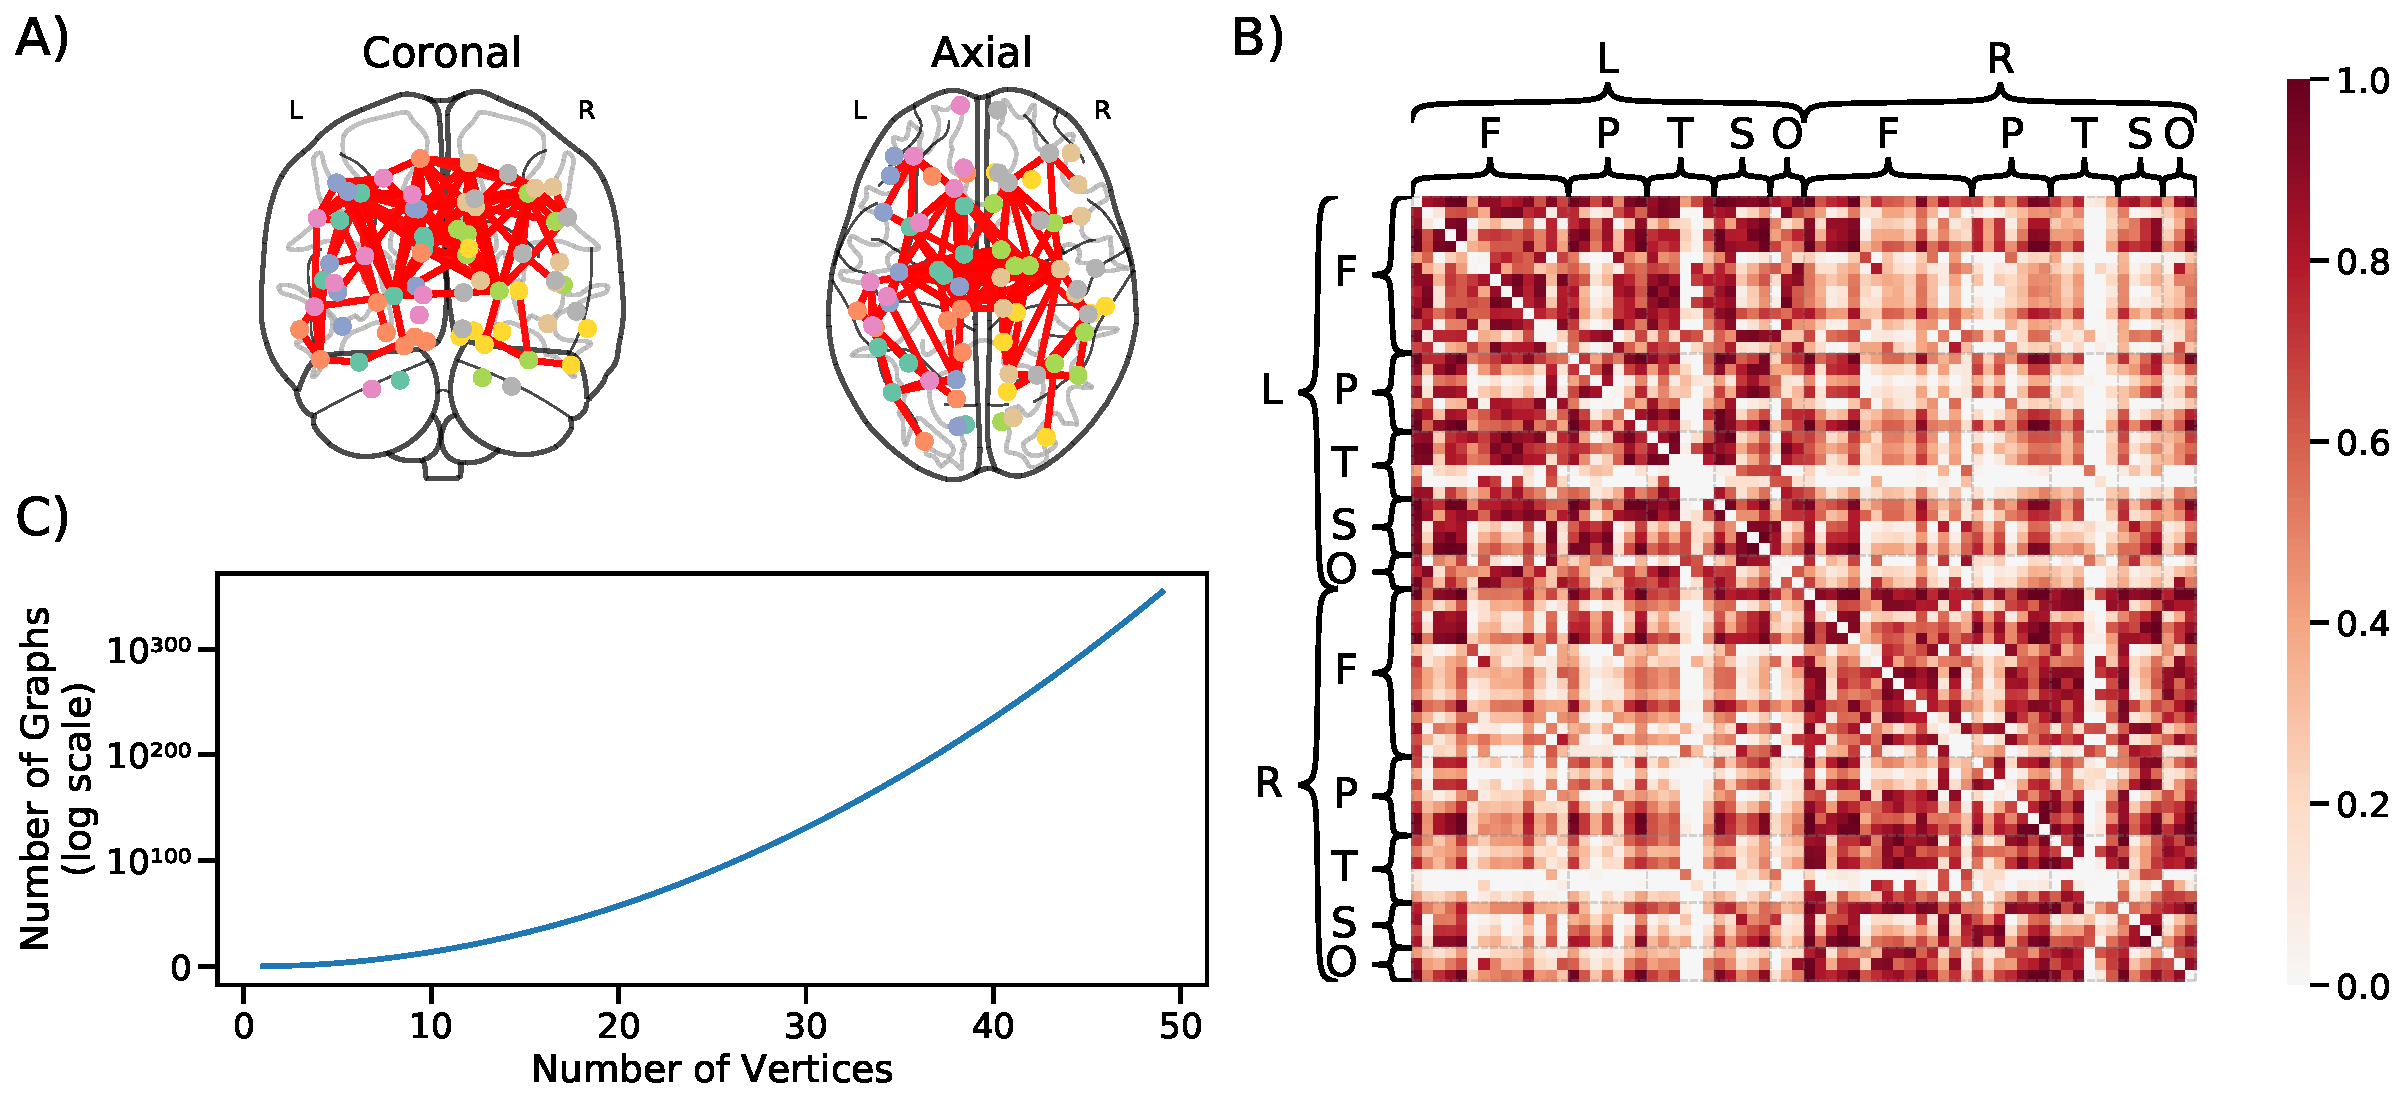
\includegraphics[width=\textwidth]{figures/dnd/intro}
    \caption
    [Different Representations of a Connectome.]
    {\textbf{Different Representations of a Connectome.} 
    Human structural connectome estimated from averaging 1059 human connectomes from the Human Connectome Project \cite{hcp1}.
    Vertices represent regions of the brain, and are assigned into right (R) and left (L) hemispheres and then further assigned into frontal (F), occipital (O), parietal (P), and temporal (T), and subcortical structures (S). 
    \textbf{a.} Connectivity shown in the coronal and axial views. Dots corresponds to the center-of-mass of the a region, lines correspond to connections, and line thickness corresponds to magnitude of the connection. Only the largest 5\% of edges are shown for visualization purposes. Note that infinitely many spatial arrangement of the vertices exist, and only one particular arrangement is being shown.
    \textbf{b.} Connectivity of the average structural connectome shown as an adjacency matrix, $\A$. The rows and columns are organized by hemisphere then further organized by sub-structures. However, given any permutation matrix $\Pbf$, the permuted adjacency matrix $\Pbf\A\Pbf^\top$ is still a valid matrix of original connectome. For a graph with $n$ vertices, there are $n^2$ permutations.
    \textbf{c.} The number of unique graphs grows exponentially as the number of vertices increases. The large number of graphs motivate statistical analysis to characterize and describe connectomes.
    } 
    \label{fig:intro_fig}
\end{figure} 
\section{Representations}\label{sec:representations}
Due to the flexibility of networks, different representations of the connectomes can be studied, which we organize into four categories. In the following sections, we first formally define a network and then describe the four different frameworks of studying connectomics data. All frameworks provide complementary insights and understanding of the connectomes. 

\subsection{Graph/Network}
\label{sec:unwt_graph}
A graph, or network, $\mathcal{G}$, is defined as an ordered set of vertices and edges $(V, E)$ where $V$ is the vertex set, and $E$, the set of edges, is a subset of the Cartesian product of $V \times V$. That is, a graph has at most a single edge for each pair of unique vertices. A vertex set is represented as $V=\{1, 2, \ldots, n\}$ where $|V| = n$, and an edge exists between vertices $i$ and $j$ if $(i, j)\in E$. An unweighted graph is a graph in which we are only concerned with the presence (or absence) of an edge. Each graph has an associated adjacency matrix $\A \in \left\{0, 1\right\}^{n\times n}$ where $\A_{ij}$ represents the presence (or absence) of the edge between nodes $i$ and $j$. Note that $\A$ provides a unique representation of $\mathcal{G}$; that is, there exists a $1$-to-$1$ relationship between a graph and its adjacency matrix. 

The above definition can be further extended in two ways: 
\begin{enumerate}
    \item Weighted graphs - the edges can take on arbitrary values, typically a real number. For example, the edge weight in human structural connectomes are non-negative integers that represent the number of estimated neuronal fibers that traverse from one region of the brain to another. Thus, each weighted graph has an adjacency matrix $\A\in\RR^{n \times n}$ where $\A_{ij}$ represents the edge weight.
    \item Directed graphs - $E$ is now an \textit{ordered} set of edges. Each edge has an associated direction, and a directed edge exists between vertices $i$ and $j$ if $(i,j)\in E$. In undirected graphs, the associated adjacency matrix $\A$ is symmetric, but in directed graphs, $\A$ is not necessarily symmetric, that is, it is possible that $\A_{ij}\neq\A_{ji}$, for any $i, j\in V$.
\end{enumerate}

For the remainder of the paper, graphs are considered undirected and unweighted and with no self-loops, that is $\text{diag}(\A) = \Vec{0}$, unless specified otherwise.

\subsection{Bag of Features}\label{sec:bag-of-features}
Network statistics, or features, are abstract representations that capture either global or local structures of a network \cite{priebe_coppersmith_rukhin_2010,mhembere2013computing}. This method computes a set of network statistics for each network, and analyzes differences between, or among, populations. For example, when comparing populations of networks from healthy and individuals with depression, the difference in global clustering coefficient, which measures how likely vertices tend to cluster together, can be computed \cite{Bullmore2009-yj}. These network statistics have enjoyed applications in many connectomics studies that compare different populations of networks \cite{bullmore2011brain, ghoshdastidar2017two}. However, there are infinitely number of such statistics, and we lack general guidance in which statistics to compute. Furthermore, no set of network statistics can adequately characterize a network \cite{chen2018same,matejka2017same}. These considerable shortcomings further motivates the use of other representations of networks, and below examples demonstrate the shortcomings of studying bags of features.

\subsubsection{Non-identifiability of graph features}
Summary statistics, such as the mean, variance, and correlation, are often used to describe real valued datasets, which can be insightful in understanding the data. However, the Anscombe's quartet illustrates four drastically different distributions of eleven points that have the same summary statistics \cite{anscombe1973graphs}. This suggest that any small number of summary statistics can fail to meaningfully characterize the data. 

In network analysis, variety of network level statistics can be computed to summarize networks. Similar to the Anscombe's quartet, networks with different topologies can have the same network features as shown in Figure \ref{fig:exp5}. These four networks have the same number of vertices, edges, triangles, and global clustering coefficient, but have different properties such as connectedness and symmetry. Other works have also explored the distributions of network statistics \cite{chen2018same,matejka2017same}. 

\begin{figure}
    \centering
    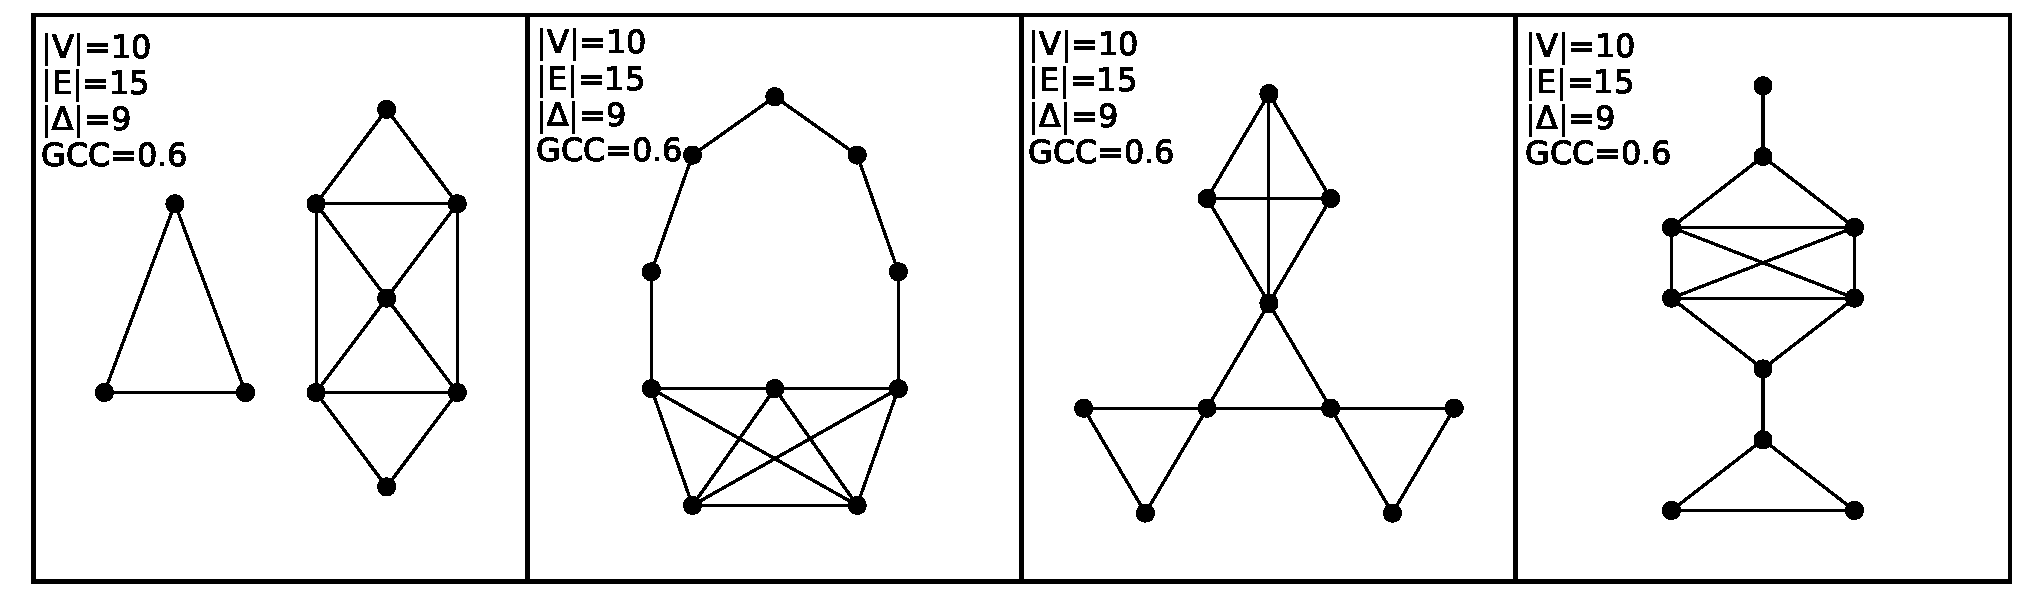
\includegraphics[width=.9\textwidth]{figures/dnd/exp5_10nodes_row}
    \caption{
    \textbf{Four Networks with Same Network Statistics.} Each network has 10 vertices ($\abs{V}$), 15 edges ($\abs{E}$), 9 triangles ($\abs{\Delta}$), and the global clustering coefficient (GCC) is 0.6. However these graphs have distinctive topologies. For example, the left-most network is disconnected, while others are connected. This suggest that given a small set of network statistics, one cannot identify from which network the features are computed.
    }
    \label{fig:exp5}
\end{figure}

\subsubsection{Network features are correlated and relatively uninformative}
We consider all non-isomorphic, undirected, binary networks with 10 vertices, which results in $\approx12$ million networks. Formally, $\mathcal{G}$ and $\mathcal{H}$ are isomorphic networks when there exists a vertex permutation function $f:V(\mathcal{G})\rightarrow V(\mathcal{H})$ such that if edge $(u,v)\in E(\mathcal{G})$, then $(f(u), f(v))\in E(\mathcal{H})$. Only non-isomorphic networks are considered since isomorphic networks have identical network features.

For each network, the following six graph network statistics are computed: 1) average path length (APL), 2) global clustering coefficient (GCC), 3) average clustering coefficient (ACC), 4) global efficiency (GE), 5) local efficiency (LE), and 6) modularity. These statistics are some of the most commonly computed statistics \cite{sporns2005human,Bullmore2009-yj}. The distribution of network statistics are plotted against modularity. 
The top row of Figure \ref{fig:exp6} shows that all of the network features are highly correlated with modularity.
We then constrain the networks in two different ways. First, we consider all networks with $20 \pm 2$ edges. Second, we choose a ``base'' network at random with 20 edges, and then identify all networks with no more than 3 edges different from the  base network. The distribution of each of the above network statistics on this subset of networks are computed for both constraints. The middle and bottom rows of Figure \ref{fig:exp6} show that constraining the networks in these ways hardly constrains the network features at all. Similar pattern is shown in the analysis of HCP data as shown in Supplemental Appendix \ref{sec:bag-of-features-hcp}. Changing only a few edges on a network can yield a network with almost any possible configuration according to these statistics, and therefore are inadequate to characterize these populations. Thus, when any given metric is correlated with a covariate of interest, so are many other metrics. Thus, claiming that a particular property of the brain ``explains'' a given phenotypic property of a person is spurious reasoning.

\begin{figure} 
    \centering
    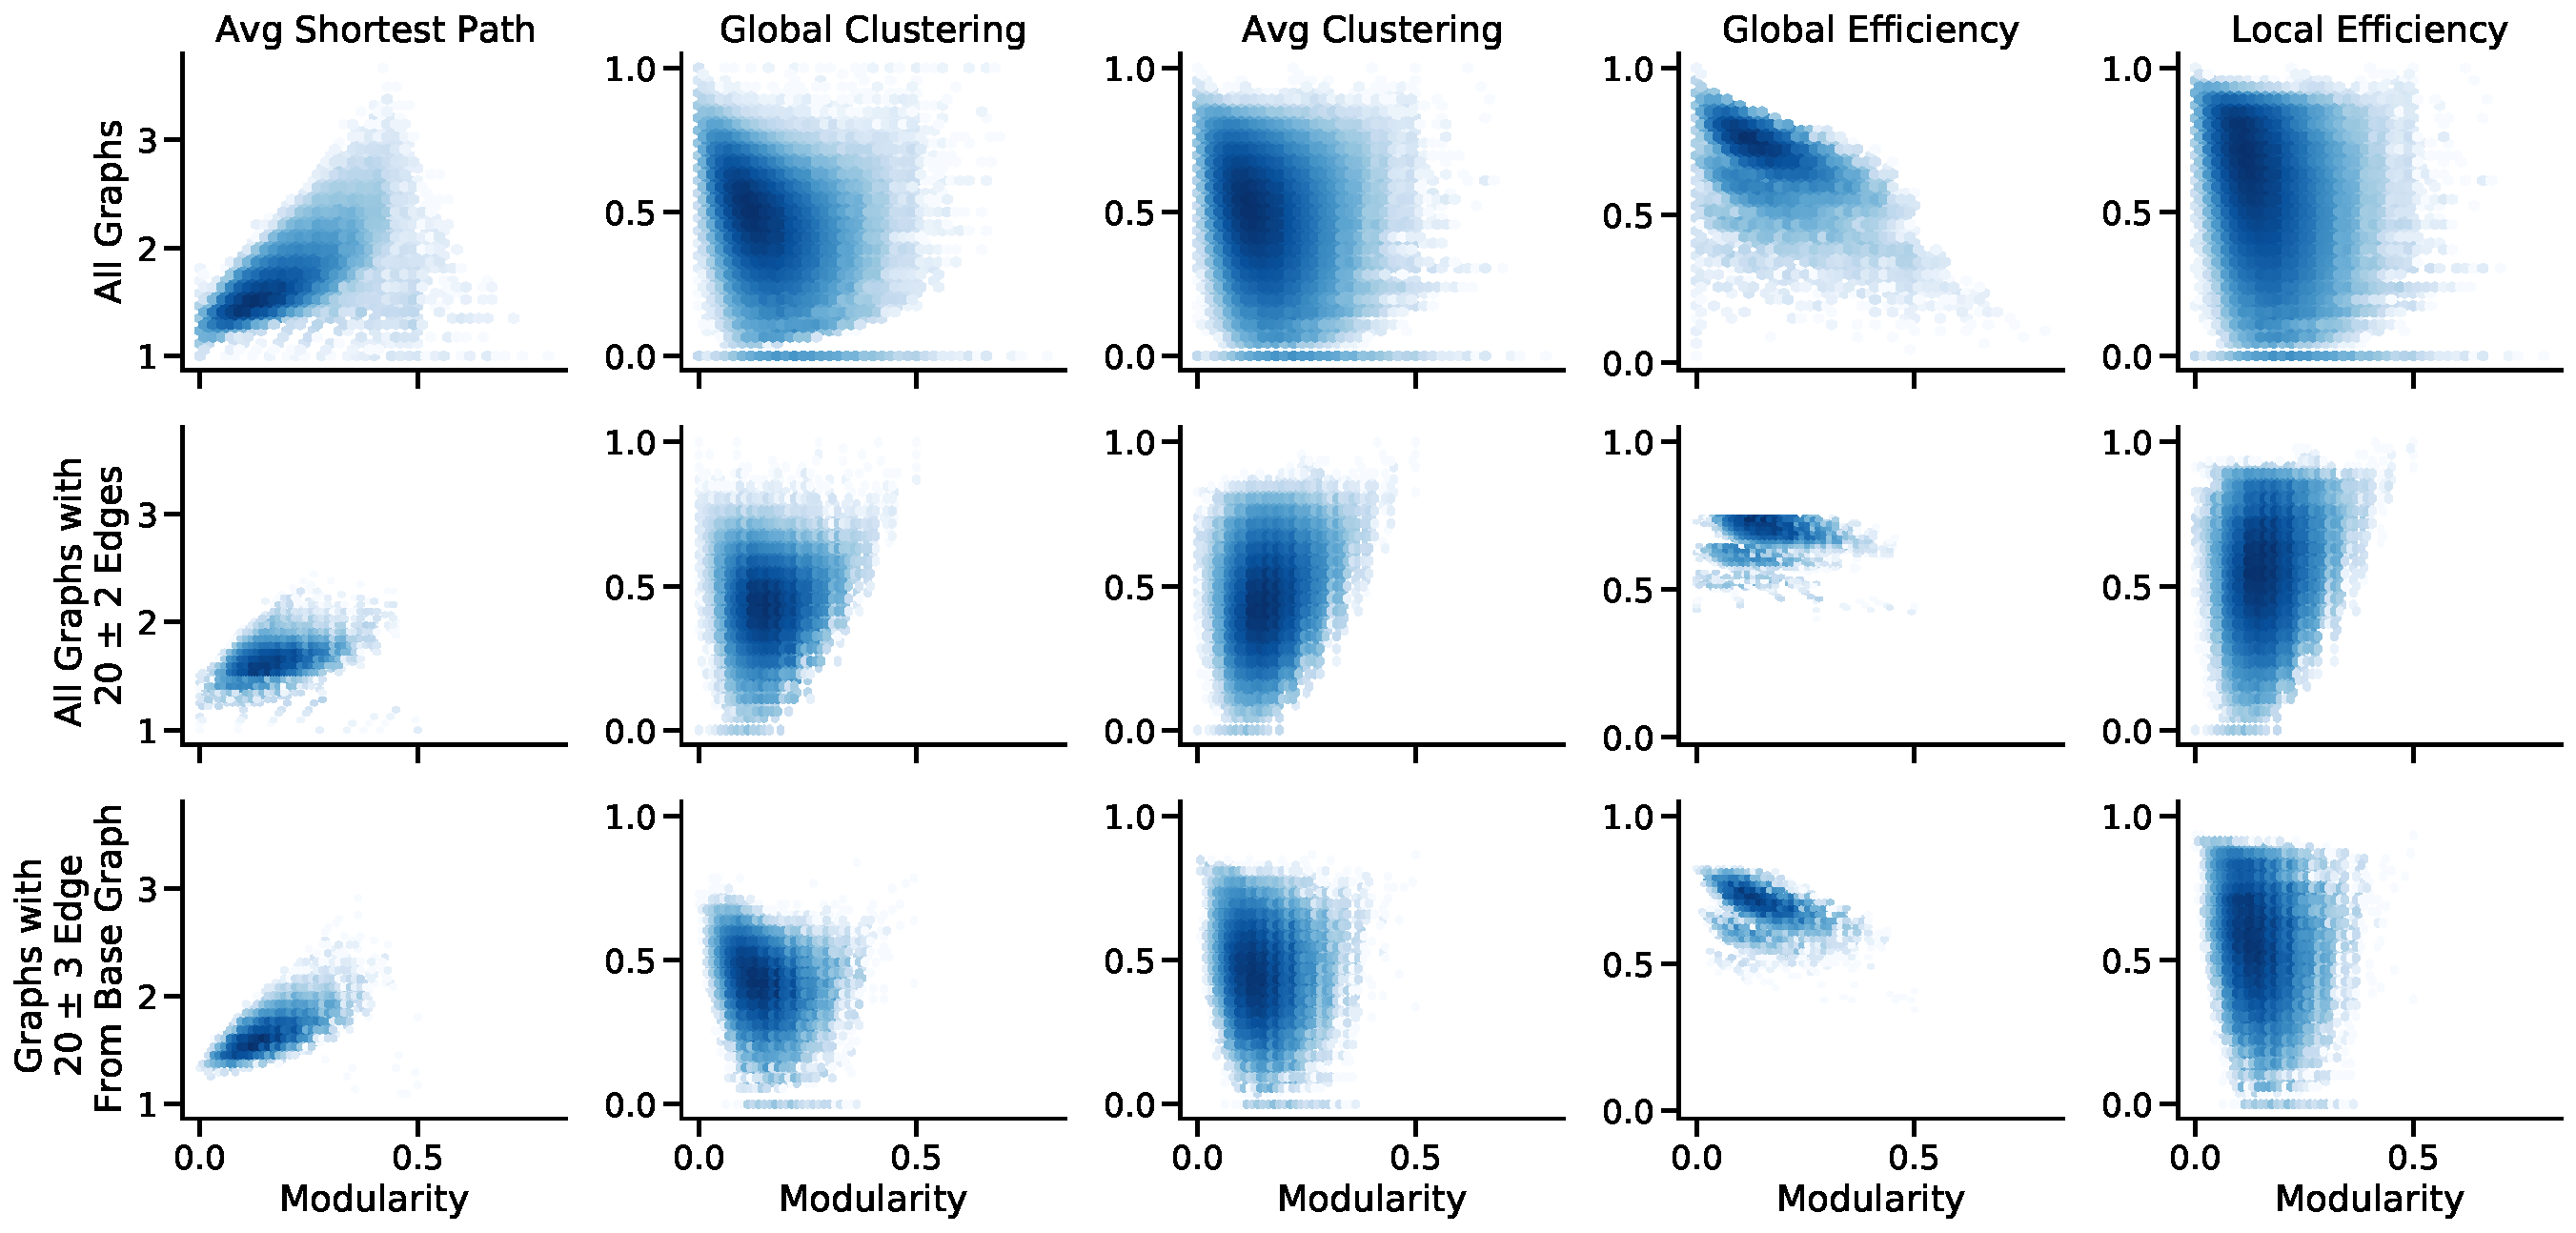
\includegraphics[width=\textwidth]{figures/dnd/density_num_edge_20_row}
    \caption{\textbf{Density plots of network statistics.} \textit{(Top Row)} The distributions of networks statistics for all possible 10-node networks are shown. \textit{(Middle Row)} Networks are constrained by only considering all networks with $20 \pm 2$ edges. \textit{(Bottom Row)} A base graph with $20$ edges is chosen at random, and only networks that have differences up to $3$ edges are considered. In both constrained set of networks, the distribution of these network statistics remains essentially unchanged. In other words, changing only a few edges on a network can yield a network with almost any possible configuration according to these statistics. }
    \label{fig:exp6}
\end{figure}

% \begin{summary}[SUMMARY POINTS]
% Networks with very different topologies can have the same values of network statistics and cannot be used to identify a specific network. Additionally, when any given metric is correlated with a covariate of interest, so are many other metrics. Thus, claiming that a particular property of the brain ``explains'' a given phenotypic property of a person is spurious reasoning. These two experiments further motivate more principled and statistically grounded analysis framework. 
% \end{summary}

\subsection{Bag of Edges}\label{sec:bag_of_edges}
In this approach, the edges of connectomes are studied. Most commonly, each edge is studied independently, while ignoring any interactions between edges \cite{Craddock2013-qs,Varoquaux2013-hy,zhang2018mapping}. Univariate edge-wise testing can reveal easily interpretable relationships between specific edges and covariates through hypothesis testing. However, edge-wise testing requires performing multiple hypothesis tests, and multiple comparisons must be corrected to control the false positive rate \cite{Genovese2002-yq,Efron2008-zq}. While certain methods, such as Benjamini–Hochberg corrections, have strong theoretical guarantees, they require assumptions about the data, such as independence, that connectomics data do not satisfy \cite{Zalesky2010-ox,Benjamini1995-ij,Simes1986-gn}. On the other hand, Bonferroni corrections are considered too conservative, and, therefore, lack the sensitivity for connectomics \cite{Simes1986-gn}.

More intricate methods represent each connectome as a long vector containing all of its edges \cite{richiardi2011decoding, amico2017mapping}. Vector representations can allow for correlation of edges and direct application of common machine learning algorithms, but still discards the structural information in networks.

\subsection{Bag of Vertices}\label{sec:bag_of_nodes}
In this approach, the vertices of connectomes are analyzed while leveraging structural information, typically global structures, of the graphs. 
A common approach embeds the connectomes to learn a low-dimensional and Euclidean representation of the vertices \cite{grover2016node2vec, athreya2017statistical, arroyo2019inference}. Algorithms that operate on Euclidean data (e.g. Gaussian Mixture Model ($\gmm$) for clustering vertices, random forests for classifying vertices, multivariate hypothesis tests for testing for differences between vertices) can be employed for subsequent analysis \cite{priebe2017semiparametric, tang2018connectome}. 

\subsection{Bag of Communities}
Networks often contain structural information such as communities, which are subsets of vertices that behave similarly. For example, similar vertices can be defined by those that are more likely to be connected with each other than to other vertices.
The set of communities that comprise a network, called community structure, can describe both the local and global patterns of the network. At local-scale, we can examine the properties of vertices that are within the same community. At global-scale, we can measure associations between connectivity patterns of communities across groups or other covariates \cite{faskowitz2018weighted, kim2019graph, arroyo2020simultaneous}. Furthermore, the community structure in spatial resolution connectomes from human MRI can be used to delineate regions of the brain, called parcellations \cite{thirion2014fmri}.

Community detection in networks have been studied extensively \cite{newman2013spectral, fortunato2016community}. Typically, the community structure is identified by modularity optimization methods \cite{clauset2004finding, blondel2008fast}. In this paper, we present spectral methods that rely on statistical models for community detection, which have strong statistical guarantees for recovering true communities \cite{sussman2012consistent, lyzinski2016community, athreya2017statistical, arroyo2019inference}.
It is important to note that analysis of communities depends on the performance of the community detection algorithms.

\subsection{Bag of Networks}
In this approach, one or more groups of networks are studied in various settings, such as one- and two-sample hypothesis testing, and classification, using some representation of networks. For example, bag of vertices representation can be used to test whether two networks are different \cite{tang2017nonparametric, tang2017semiparametric}. For studying more than two networks, geometry in the space of the networks is defined and are represented in that geometry, which are then used for finding differences across groups \cite{ginestet2017hypothesis, xia2019matrix, arroyo2019inference}.

Another group of methods finds subsets of vertices, or a subgraph, that contain the most information about certain covariates \cite{vogelstein2012graph, wang2018signal,  relion2019network, wang2019symmetric, guha2020bayesian}. Estimating signal subgraphs is useful since networks can be extremely large (i.e. millions of vertices), which present computational challenges, and can potentially improve the performance of subsequent inference tasks, such as classification. 
Different approaches for finding the subgraph have been proposed, but all approaches leverage the network topologies inherent in connectomics data. 

\begin{table}
\caption{Notations and symbols used in this paper}\label{tab1}
\begin{center}
\begin{tabular}{|@{}l|c@{}|@{}l|c@{}|}
\hline
Symbols & Description & Symbols & Description\\
\hline
$[n]$ & $\{1, 2, \ldots, n\}$ & $\Pbf$ & Edge connectivity probability matrix\\
$\mathcal{G}$ & Graph & $\B$ & Block connectivity probability matrix\\
$n$ & Number of nodes & $\vec{\tau}$ & Vertex community assignment vector\\
$\A$ & Adjacency matrix & $\M$ & Edge community assignment matrix\\
$\A_i$ & $i$-th row of $\A$ & $\X$ & Latent position matrix\\
$\A_{ij}$ & $(i,j)$ entry of $\A$ & $\hat{\X}$ & Estimated latent position matrix\\
$\A^{(l)}$ & $l$-th element in sequence of $\A$ & &\\
\hline
\end{tabular}
\end{center}
\end{table}

\section{Statistical Models}\label{sec:models}
Connectomes can be modelled using statistical models designed for network data \cite{ goldenberg2010survey, kolaczyk2014statistical}. Statistical models consider the entire network as a random variable, including the inherent structure, dependencies within networks, and the noise in observed data. 
Thus, statistical models can formalize detecting similarities or differences for each of the representations in Section \ref{sec:representations}.
This section provides an overview of many statistical models for network data, including those designed for representing single and multiple networks. 

Section \ref{sec:single_graph_models} provides an overview of single graph models that have been extensively studied as well as recently introduced models in the order of least to greatest complexity. Figure \ref{fig:models}a shows the relationship between all the single graph models presented in this paper. Section \ref{sec:multi_graph_models} provides an overview of some models for multiple networks. While other statistical models for multiple network data exist \cite{zhang2018network, wang2019joint, nielsen2018multiple, Durante2017-fz}, we focus on  some recent models that are used in spectral inference for connectomics data. In Appendix \ref{sec:model_extensions}, we describe some extensions to these models. 

\begin{figure}
    \centering
    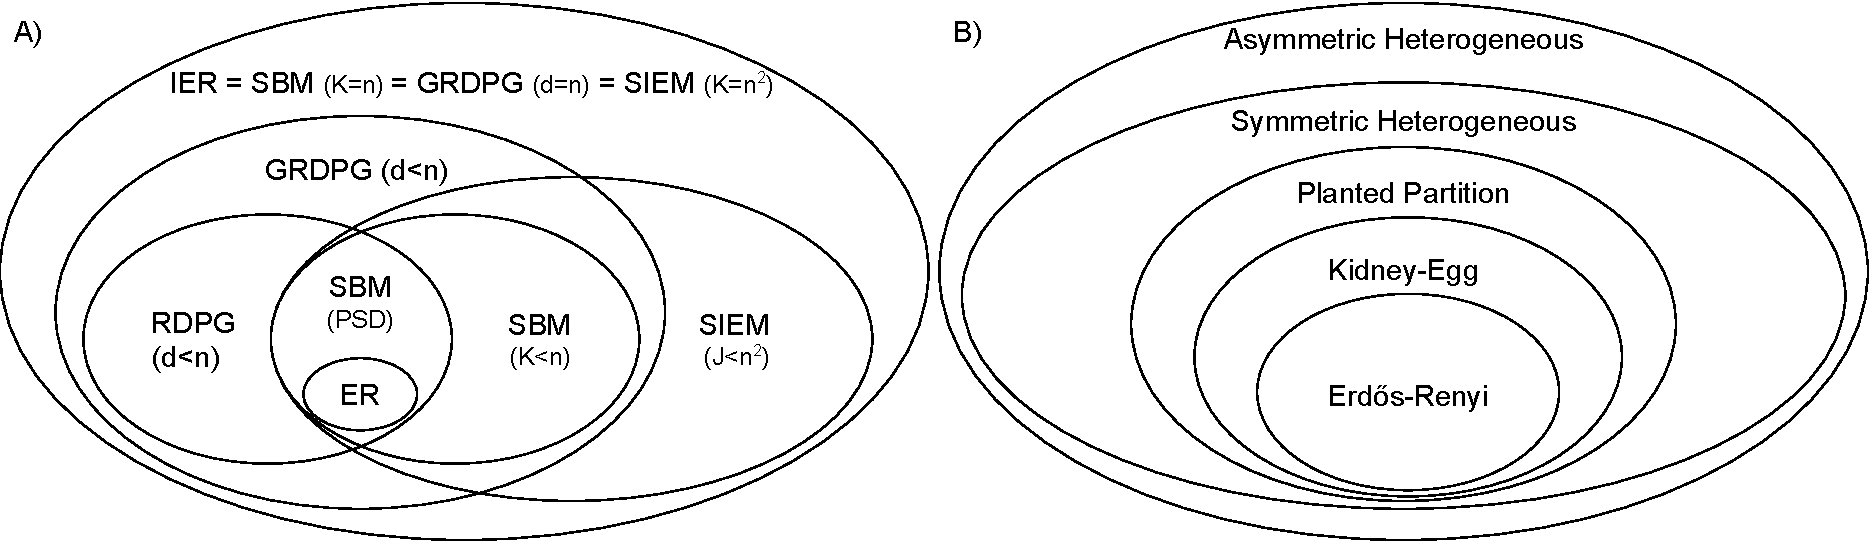
\includegraphics[width=\textwidth]{figures/dnd/models_combined}
    \caption
    [Hierarchical Relationships of Statistical Models]
    {\textbf{Hierarchical Relationships of Statistical Models} 
    \textbf{(a)} Relationships among all the single-graph statistical models. Erd\H os-R\'enyi ($\er$) model is a stochastic block model ($\sbm$) with one community. $\sbm$ with a positive semidefinite block probability matrix $\B$ is also a random dot product graph ($\rdpg$). Any $\sbm$, $\rdpg$, and some structured independent edge model ($\siem$) can be represented as $d$-dimensional generalized random dot product graph ($\grdpg$) with $d$ less than number of vertices $n$. Inhomogenous Erd\H os-R\'enyi ($\ier$) model is equivalent to a $n$-block $\sbm$, $n$-dimensional $\grdpg$, and $n^2$-group $\siem$.
    \textbf{(b)} Relationships among the two-block $\sbm$ models. The most complex model is the asymmetric heterogeneous $\sbm$, and the simplest model is the $\er$, which is a degenerate case of 2-block $\sbm$.}
    \label{fig:models}
\end{figure}

\subsection{Single Graph Models}\label{sec:single_graph_models}
\subsubsection{Erd\H os-R\'enyi Random Graphs (ER)}\label{sec:uer}
The simplest random graph model is the $\mathsf{Erd\ddot{o}s-R\acute{e}nyi~(ER)}$ model \cite{Erdos1959-zf}. For a given set of $n$ vertices, each distinct pair of vertices are connected independently with probability $p \in [0, 1]$. Specifically, $\A \sim\er_n(p)$ if $\A$ has entries $\A_{ij}\sim\bern(p)$ for $i, j \in [n]$. While the $\er$ model is not representative of real data, it has been studied extensively since many of its properties can be solved exactly  \cite{newman2003random,Rukhin2010}.  

\subsubsection{Stochastic Block Model (SBM)}\label{sec:usbm}
First introduced in \cite{holland1983stochastic}, $\sbm$ is a model that can produce graphs with vertices grouped into $K$ communities \cite{Rohe2011-ha,sussman2012consistent,Wasserman1987-tw}. There are two simple variations of the $\sbm$ in which the vertex assignment vector $\vec \tau \in \left\{1, \hdots, K\right\}^n$ is known \textit{a priori}, and where $\vec \tau$ is not known. 
In both cases, a symmetric $K \times K$ block connectivity probability matrix $\B$ with entries in $[0,1]^{K \times K}$ governs the probability of an edge between vertices given their block memberships. 

If $\vec \tau \in \left\{1, \hdots, K\right\}^n$ is known \textit{a priori}, the \textit{a priori} $\sbm$ is parametrized only by the block connectivity matrix $\B$, and the model is $\A \sim \sbm_n(\vec \tau,\B)$ if $\A$ has entries $\A_{ij} \sim \bern(\B_{kl})$ where $\tau_i = k, \tau_j = l$, for $i, j \in [n]$, and $k, l \in [K]$. In the case where $\vec \tau$ is not known, the \textit{a posteriori} $\sbm$ is additionally parameterized by a block membership probability vector $\vec{\pi} = [\pi_1,\dots,\pi_K]^\top$ on the probability simplex.
The model is $\A \sim \sbm_n(\vec \pi,\B)$ if $\A$ has entries $\A_{ij} \big | k=\tau_i, l=\tau_j \sim \bern(\B_{kl})$, where $\tau_i {\sim} \multinomial(\vec \pi)$ for $i = 1, \hdots, n$. 

Throughout the context of this paper, we will focus particularly on a few variations of the two-block $\sbm$ ($K=2$) with block connectivity matrix $\B = \begin{bmatrix}a & b \\ c & d \end{bmatrix}$, abbreviated as $\B = [a, b; c, d]$. The common variants include:
\begin{enumerate}
    \item $\mathsf{Kidney-Egg}$: $b = c = d$. In this model, one of the blocks has edges with a different probability than the others, but the remaining blocks are homogeneous, where $a \neq b$. Furthermore, when $b > a$, the model is referred to as core-periphery $\sbm$.
    \item $\mathsf{Planted~Partition}$: $a = d$ and $b = c$. In this model, the within-block edges share a common probability $a$, and the between-block edges share a common probability $b$, where $a \neq b$.
    \item $\mathsf{Symmetric~ Heterogeneous}$: $b = c$. In this model, the between-block edges share a common probability $b$, but the within-block edges have a disparate probabilities, where $a \neq b \neq d$. 
    \item $\mathsf{Asymmetric~ Heterogeneous}$: $a \neq b \neq c \neq d$. In this directed model, every block has a unique probability.
    \item $\mathsf{Erd\ddot{o}s-R\acute{e}nyi}$: $a=b=c=d$. In this degenerate model, all blocks have a common probability, and the partitioning is irrelevant. 
    \item $\mathsf{Homophilic/Assortative/Affinity}$: $a, d > b, c$. In this model, the within-block probabilities are greater than cross-block probabilities.
    \item $\mathsf{Disassortative}$: $ b, c > a, d$. In this model, the cross-block probabilities are greater than the within-block probabilities.
\end{enumerate}
Figure \ref{fig:models}b summarizes the relationships of $\sbm$ models.

\subsubsection{Structured Independent Edge Model (SIEM)}\label{sec:usiem}
$\siem$ is a generalization of $\sbm$ that produces graphs in which edges are grouped into one of $K$ clusters. Analogous to the vertex assignment vector of the \textit{a priori} $\sbm$, the $\siem$ features an edge community assignment matrix $\M \in \left\{1, \hdots, K\right\}^{n \times n}$ which is known \textit{a priori}. Given the community assignment matrix $\M$, the $\siem$ is $\A \sim \siem_n(\M, \vec p)$ if $\A_{ij} {\sim}\bern(p_k)$ where $\M_{ij} = k$, for $i, j \in [n]$ and $k \in [K]$. $\vec p = [p_1, \hdots, p_K]^\top \in [0, 1]^K$ is the edge probability vector which governs the probability of an edge between vertices. 

The \textit{a priori} $\sbm$ is a special case of $\siem$ in which edges are assigned to blocks $\M$ which respect the vertex assignment vector $\vec \tau$. For the purposes of this paper, we will consider a case that frequently comes up in neuroimaging, the $\mathsf{Homotopic~ SIEM}$, in which each vertex has a matched ``pair'' amongst other vertices. The edges corresponding to a pair $\M_{ij} = 2$ where $(v_i, v_j)$ are a pair of vertices sharing a property, and the edges corresponding to a non-pair are $\M_{ij} = 1$. A matched pair of vertices, for instance, could be homotopic brain regions (two brain regions with similar function but in opposing hemispheres of the brain).

\subsubsection{Random Dot Product Graphs (RDPG)}\label{sec:rdpg}
$\rdpg$ belongs to the class of latent position random graphs \cite{hoff2002latent}. In a latent position graph, every vertex has associated to it a (typically unobserved) \textit{latent position} in some space $\mathcal{X}$, and the probability of connection between vertices $i$ and $j$ are given by a link function. In $\rdpg$, the space $\mathcal{X}$ is a constrained subspace of Euclidean space $\RR^d$ and the link function is the dot product \cite{Young2007-vu,scheinerman2010modeling,Sussman2014-zq}. Thus, in a $d-$dimensional $\rdpg$ with $n$ vertices, the matrix $\X\in \RR^{n\times d}$ whose rows are the latent positions, and the matrix of connection probabilities is given by $\Pbf=\X\X^\top$, which is positive semidefinite. The model is $\A\sim \rdpg_n(\X)$ if the adjacency matrix $\A$ has entries $\A_{ij} \sim \bern(\X_i\X_j^\top)$.
Subsequent inference tasks include community detection \cite{sussman2012consistent}, vertex classification \cite{tang2013}, or two-sample hypothesis testing for graphs with matched and non-matched vertices for a pair of graphs  \cite{priebe2019two,tang2017nonparametric,tang2017semiparametric}.

The $\rdpg$ is a flexible model, and other models of interest can be seen as special cases of the $\rdpg$. A $\sbm$ whose block connectivity matrix $\B$ is positive semi-definite is a $\rdpg$ with $K$ distinct latent positions. Thus, a $\sbm$ with $K$ blocks can be represented with a latent position matrix $\X\in\RR^{n\times d}$, with $d\leq K$, where there are only $K$ different rows of $\X$, and letting $\X_{\mathcal{U}}\in\RR^{K\times d}$ be the matrix with the subset of the rows $\mathcal{U}$ where each row is the latent position for a block, then the block connectivity matrix is $\B= \X_\mathcal{U}\X_\mathcal{U}^\top \in\RR^{K\times K}$. More generally, the $\rdpg$ can represent other models with more complex structures, such as mixed memberships \cite{Airoldi2008-tp} or hierarchical communities \cite{Lyzinski2017-cq}.

\subsubsection{Generalized Random Dot Product Graphs (GRDPG)}\label{sec:grdpg}
Unlike $\rdpg$ model, $\grdpg$ does not assume that $\Pbf$ is a positive semidefinite probability matrix  \cite{rubin2017statistical}. In this model, the edge probability matrix is given by $\Pbf=\X \I_{pq}\X^\top$, and $\A\sim\grdpg_n(
\X, p, q)$ if $\A_{ij}\sim\bern(\X_i\I_{pq}\X_j^\top)$ where $\I_{pq}=\textrm{diag}(1, \ldots, 1, -1, \ldots, -1)$  with $p$ ones followed by $q$ minus ones on its diagonal, and where $p \geq 1$ and $q \geq 0$ are two integers satisfying $p + q = d$.

The $\grdpg$ generalizes all of the previous models. When $q=0$, $\grdpg$ reduces to a $\rdpg$ model. To represent any $\sbm$ as $\grdpg$, let $p\geq 1, q\geq 0$ be the number of positive and negative eigenvalues of the block connectivity matrix $\B\in\RR^{K\times K}$, respectively. The block matrix can be represented as $\B = \X_\mathcal{U}\I_{pq}\X_\mathcal{U}^\top$.

\subsubsection{Inhomogenous Erd\H os-R\'enyi Random Graphs (IER)}\label{sec:uierrg}
The $\mathsf{Inhomogenous~Erd\ddot{o}s-R\acute{e}nyi~(IER)}$ is a model where each pair of nodes has a unique probability of an edge existing between the two, and is therefore the most general independent edge model. For a given set of $n$ vertices, the $\ier$ is parametrized by a matrix $\Pbf \in [0, 1]^{n \times n}$, where $\Pbf_{ij}$ is the probability of an edge connecting vertices $v_i, v_j$ where $i, j \in [n]$. That is, $\A \sim \ier_n(\Pbf)$ if $\A$ has entries $\A_{ij}\sim \bern(\Pbf_{ij})$ for $i, j \in [n]$. $\ier$ cannot be estimated from a single graph, as there are $n\choose 2$ unknowns (the probabilities) with $n\choose 2$ total observations (the edges).

Note that all single graph models are special cases of $\ier$. Additionally, $\sbm$ with $K=n$, $\siem$ with $K=n^2$, and $\grdpg$ with $d=n$ are equivalent to an $\ier$ model.

\subsection{Multiple Graph Models}\label{sec:multi_graph_models}
A common idea in statistical models for multiple graphs is a shared latent space that contain structural information common to all graphs. The two models presented in this section constrain the shared latent space in different ways to describe the heterogeneity in graphs, which results in sensitivity to different kinds of heterogeneity. The advantages and disadvantages of each model are highlighted in Section \ref{sec:multi_app}.

In the following models, consider a sample of $m$ observed graphs $\mathcal{G}^{(1)}, \mathcal{G}^{(2)}, \ldots, \mathcal{G}^{(m)}$  and their associated adjacency matrices, $\A^{(1)}, \A^{(2)}, \ldots, \A^{(m)}\in\RR^{n\times n}$ with $n$ vertices that are identical and shared across all graphs. 

\subsubsection{Joint Random Dot Product Graphs (JRDPG)}
In this model, we consider a collection of $m$ $\rdpg$s all with the same generating latent positions. Similar to a $\rdpg$, given an appropriately constrained Euclidean subspace $\RR^d$, the model is parameterized by a latent positions matrix $\X\in\RR^{n\times d}$ where $d \ll n$. The model is $\left(\A^{(1)}, \A^{(2)}, \ldots, \A^{(m)}\right)\sim \jrdpg(\X)$ where $\A_{ij}^{(l)}\sim \bern(\X_i\X_j^\top)$ for all $i, j \in [n]$ and $l\in [m]$. Each graph has marginal distribution $\A^{(l)}\sim\rdpg(\X)$ for all $l \in [m]$, meaning that the matrices $\A^{(1)}, \ldots,\A^{(m)}$ are conditionally independent given $\X$ \cite{athreya2017statistical,levin2017central}. While the model assumes that the latent positions for the graphs are the same, we note that this assumption is likely violated in heterogeneous networks, but still remains a very useful model as shown in Section \ref{sec:multi_app}.

\subsubsection{Common Subspace Independent-Edge Model (COSIE)} \label{sec:cosie}
In this model, the heterogeneous networks are described via a shared latent structure on the vertices, but also permits sufficient heterogeneity via individual matrices for each graph  \cite{arroyo2019inference}.
The model is parameterized by a  matrix $\V\in\RR^{n\times d}$ with orthonormal columns, 
where $n$ is the number of vertices and $d\ll n$, and  symmetric individual score matrices $\R^{(i)}\in\RR^{d\times d}$. The matrix $\V$ characterizes a low-rank common subspace, and is related to the latent positions for the vertices, and the score matrices incorporate individual differences to model the heterogeneity of the graphs. The model is denoted by $\left(\A^{(1)}, \ldots, \A^{(m)}\right)\sim \cosie(\V; \R^{(1)}, \ldots, \R^{(m)})$ where $\A_{ij}^{(l)} \sim \bern(\mathbf{P}^{(l)}_{ij})$ for all $i, j\in [n], i < j$, and $\mathbf{P}^{(l)}=\V\R^{(l)}\V^\top$. This factorization of the expected adjacency matrices is related to other decompositions for multiple matrices into population singular vectors or eigenvectors and individual parameters \cite{afshin2012enhancing,crainiceanu2011population,lock2013joint,wang2019common}.

\subsubsection{Correlated Models} \label{sec:correlated-graphs}
Finally, we are interested in graph models for a pair of graphs, $\mathcal{G}_1$ and $\mathcal{G}_2$, where the two graphs are said to be correlated; that is, the edges adjoining incident vertices have a non-zero correlation. Correlated graph models have numerous applications, such as when a graph is estimated repeatedly for the same source at different points in time.

\paragraph{Correlated $(\Pbf,\Q)$}

The $\mathbf{R}$-correlated $(\Pbf, \Q)$ model \cite{lyzinski2017matchability} with parameters $\mathbf{R}, \Pbf, \Q\in[0,1]^{n\times n}$, denoted as $\mathrm{CorrER}(\Pbf, \Q, \mathbf{R})$, produces two graphs $\mathcal{G}_1$ and $\mathcal{G}_2$ with adjacency matrices $\A^{(1)}, \A^{(2)}$ such that each graph is marginally an inhomogeneous Erd\H{o}s-R\'enyi with $\A^{(1)} \sim \ier(\Pbf)$, $\A^{(2)}\sim \ier(\Q)$, but the  pairs of corresponding edges have Pearson correlation  encoded in the matrix $\mathbf{R}$ such that 
$$\mathbf{R}_{ij} = \text{Corr}(\A^{(1)}, \A^{(2)})= \frac{\mathbb{P}(\A^{(1)}_{ij}=\A^{(2)}_{ij}=1)-\Pbf_{ij}\Q_{ij}}{\sqrt{\Pbf_{ij}(1-\Pbf_{ij}) \Q_{ij}(1-\Q_{ij})}}.$$
When $\Pbf$ and $\Q$ are different, there are restrictions in the values that the correlation matrix $\mathbf{R}$ can take. In particular, if $\Pbf_{ij}\neq\Q_{ij}$  and $\Pbf>\Q$, then $\mathbf{R}_{ij}\leq \sqrt{\frac{\Q_{ij}(1-\Q_{ij})}{\Pbf_{ij}(1-\Pbf_{ij})}}$ \cite{lyzinski2017matchability}.

We are interested particularly in two special cases of the $\mathrm{CorrER}(\Pbf, \pmb Q, \pmb R)$:
\begin{enumerate}
    \item The $\rho$-correlated $\rdpg$ model arises when $\Pbf = \Q=\X\X^\top$ for some latent position matrix $\X \in \RR^{n \times d}$  as in Section \ref{sec:rdpg}, and $\pmb R = \rho \pmb 1_{n \times n}$ (that is, the matrix of edge correlations $\pmb R$ has only a single unique entry $\rho\geq 0$). We say that $\A_1, \A_2 \sim \rho\rdpg(\X)$.
    \item The $\rho$-correlated $\er$ model arises in the case where $\Pbf = \Q = p\pmb 1_{n \times n}$ (i.e.,  the probability matrix has a single unique entry $p>0$), and $\pmb R = \rho\pmb 1_{n \times n}$ (as above, the matrix of correlations has a single unique entry). We say that $\A_1, \A_2 \sim \rho\er(p)$.
\end{enumerate}
\section{Algorithms}\label{sec:algorithms}
In this section, we introduce algorithms for statistical analysis of networks. Section \ref{sec:single_algo} provides an overview of algorithms for a single graph and Section \ref{sec:multi_algo} provides an overview of algorithms designed for multiple graphs. 

% Important TODO: Check consistency of the subindex notation. Here U_d is indicating something different than in the previous section (rows of U vs a matrix with d columns?)
% Another important TODO: The definition of ASE is wrong, A is not equal to USU^T, that is the truncation to its first d eigenvectors. I'm going to change it but please make sure that there are not problems with this in the rest of the paper.


\subsection{Single Graph Algorithms}\label{sec:single_algo}
\subsubsection{Adjacency and Laplacian Spectral Embedding (ASE, LSE)} \label{sec:ase}
Given an undirected graph with adjacency matrix $\A$, the adjacency spectral embedding ($\ase$) and Laplacian spectral embedding ($\lse$) construct a representation of the vertices of the graphs into $d$ dimensions via its eigendecomposition, given by
$\A = \mathbf{U}\mathbf{S}\mathbf{U}^\top$
where $\mathbf{U}\in\RR^{n\times n}$ is the orthogonal matrix of eigenvectors and $\mathbf{S}\in\RR^{n\times n}$ is a diagonal matrix containing the eigenvalues of $\A$ ordered by magnitude, such that $|\mathbf{S}_{11}|\geq |\mathbf{S}_{22}| \geq \ldots \geq |\mathbf{S}_{nn}|$. 
 The $\ase$ of the graph into $\RR^{d}$ is defined as $\ase(\A)=\hat{\X}= \hat{\mathbf{U}}|\hat{\mathbf{S}}|^{1/2}$, where $\hat{\mathbf{U}}\in\RR^{n\times d}$ contains the first $d$ columns of $\mathbf{U}$, which correspond to the largest eigenvectors, and $\hat{\mathbf{S}}\in\RR^{d\times d}$ is the submatrix of $\mathbf{S}$ corresponding to the $d$ largest eigenvalues in magnitude. The $\lse$, of $\A$ is defined in a similar manner using the normalized Laplacian of the graph defined as $\mathbf{L} = \mathbf{D}^{-1/2}\A\mathbf{D}^{-1/2}$ where $\mathbf{D} \in\RR^{n\times n}$ is a diagonal matrix with entries $\mathbf{D}_{ii}=\sum_j\A_{ij}$. Then, the $\lse$ of the graph is given by $\lse(\A)=\ase(\mathbf{L})=\tilde \X\in\RR^{n\times d}$.
% TODONE: I changed \hat{X} to \tilde{X} for LSE to distinguish them from each other (that's what other papers commonly write them). Please check if it needs to be changed somewhere else.
% TODO@ja - corrected. Underscore means rows

% TODONE: Here the definition is also wrong, I fixed it but please check the rest
In the case of directed graphs, the eigendecomposition is not available since adjacency matrix is not symmetric, so instead we use the singular value decomposition of the adjacency matrix as $\A=\mathbf{U}\mathbf{S}\mathbf{V}^\top$, where $\mathbf{U},\mathbf{V}\in\RR^{n\times n}$ are orthogonal matrices containing the left and right singular vectors, and $\mathbf{S}\in\RR^{n\times n}$ is a non-negative diagonal matrix with the singular values. 
The $\ase$ of a directed graph results in two different latent position matrices $\hat{\X}= \hat{\mathbf{U}}\hat{\mathbf{S}}^{1/2}$ and $\hat{\Y}= \hat{\mathbf{V}}\hat{\mathbf{S}}^{1/2}$, denoted \textit{in} and \textit{out} latent positions, respectively, where $\hat{\mathbf{U}},\hat{\mathbf{V}}\in\RR^{n\times d}$ contain the $d$ columns of $\mathbf{U}$ and $\mathbf{V}$ corresponding to the $d$ leading singular vectors, and $\hat{\mathbf{S}}$ is the submatrix of $\mathbf{S}$ containing the $d$ leading singular values. 
While there exists many definitions for directed normalized Laplacian, we define it as $\mathbf{L} = \mathbf{D}^{-1/2}\A\mathbf{O}^{-1/2}$ where $\mathbf{D}_{ii} =\sum_j\A_{ij}$ and  $\mathbf{O}_{ii} =\sum_j\A_{ji}$ are the in and out degree diagonal matrices \cite{rohe2016co}. The $\lse$ of directed graph processed similarly to that of directed $\ase$. 

Spectral embedding is the first step in many subsequent inference tasks. For example, spectral clustering for community detection (Section \ref{sec:clustering_single}) can be achieved via Gaussian Mixture modeling on $\hat \X$ from either $\ase$ or $\lse$. The resulting cluster assignments can further be used to estimate the parameters for \textit{a posteriori} $\sbm$. 

For real data, the true embedding dimension $d$ is often not known and must be estimated. A general methodology for choosing the embedding dimension $d$ is to examine the scree plot of the singular values of $\A$ and look for an ``elbow'' or a ``big gap''. While many methods for choosing the threshold exist \cite{jackson2005user,chatterjee2015matrix}, we consider the method in \cite{zhu2006automatic} when applying any spectral embeddings in real data. Given $\A= \mathbf{U}\mathbf{S}\mathbf{U}^\top$ for either $\ase$ or $\lse$, the eigenvalues in $|\mathbf{S}|$ are used to estimate the embedding dimension $\hat d$ by maximizing the profile likelihood function, which determines the magnitude of the ``gap'' after first $d$ largest eigenvalues. Multiple elbows can be found by discarding the $\hat d$ number of largest eigenvalues and repeating the process with the remaining eigenvalues. For applications in connectomics, we only consider $\ceil{\log{n}}$ largest eigenvalues as input to the profile likelihood function and take the second elbow as the estimate of $\hat d$.
% \begin{align*}
%     \hat d &= \argmax_d \mathrm{ProfileLikelihood}_S(d)
% \end{align*}
% TODONE: I don't think it adds any value to display an equation like this if the exact form of the profile likelihood function is not going to appear. Maybe delete and just mention that d hat maximizes the profile likelihood (i.e. the same thing but with words).

% TODONE mention ZG(2) explicitly please, as well as log(n) as the upperbound on d, or whatever other tricks we do. this will be the only place that stuff is ever actually written down.

\subsubsection{Diagonal Augmentation}\label{sec:diag-aug}
Many connectomes have no self-loops, resulting in all zero in the diagonal entries of the adjacency matrices. When computing spectral embeddings of graphs, the zero diagonal results in increased errors in estimation \cite{tang2018connectome}. Furthermore, the sum of eigenvalues of the adjacency matrices is zero, leading to an indefinite matrix, which violate assumptions of the statistical models such as $\rdpg$. 

Diagonal augmentation ($\sct{diag-aug}$) is a method for imputing the diagonals of adjacency matrices from graphs with no self-loops \cite{marchette2011vertex,tang2018connectome,scheinerman2010modeling}. The diagonals are imputed with with the average of the non-diagonal entries of each row, which corresponds to the degree of each vertex divided by $n-1$. In the case of directed graphs, the average of in and out degree is used. Specifically, the diagonal augmented adjacency matrix is defined as $\tilde \A = \A + \tilde\D$ where $\A\in\RR^{n\times n}$, $\tilde \D \in\RR^{n\times n}$ is a diagonal matrix with entries $(\mathbf{A}\vec 1^\top + \vec 1\mathbf{A}) /2(n-1)$ where $\vec 1 \in\RR^n$ is a row vector of ones. To achieve best embedding estimation, the diagonal entries of adjacency matrices should be imputed prior to $\ase$ (in $\lse$, the diagonals are imputed via the normalized Laplacian).

\subsubsection{Pass-To-Ranks (PTR)}
Connectomes have often weighted edges, which can take on arbitrary values. Rescaling and normalizing the edge weights has been shown to increase reliability and can improve estimation of spectral embeddings \cite{Kiar188706}. Pass-to-ranks ($\ptr$) is a method for rescaling the \textit{positive} edge weights such that all edge weights are between 0 and 1, inclusive. 

Given an adjacency matrix $\A \in \Real^{n\times n}$, let $R(\A_{ij})$ be the ``rank'' of $\A_{ij}$, that is, $R(\A_{ij}) = k$ if $\A_{ij}$ is the $k^{th}$ smallest number in $\A$. The rescaled adjacency matrix, $\Tilde{\A}$, is defined as follows:
\begin{align*}
    \Tilde{\A}_{ij} &= \begin{cases}
    \frac{R(\A_{ij})}{|E|} & \text{if $\A_{ij} > 0$},\\
    0 & \text{otherwise},
    \end{cases}
\end{align*}
where $|E|$ is the number of non-zero edges. Ties in rank are broken by averaging the ranks. For spectral embedding of weighted connectomes, they are first normalized via $\ptr$, then the diagonals are imputed via $\sct{diag-aug}$ prior to $\ase$ ($\sct{diag-aug}$ is skipped for $\lse$). 

\subsubsection{Spectral Clustering for Community Detection} \label{sec:clustering_single}
One of the most common uses of spectral clustering is for community detection, in which the vertices with similar connectivity patterns are grouped together. Given the embeddings of a graph from either $\ase$ or $\lse$, classical Euclidean clustering of $\hat{\X}$ results in community structure. Central limit theorems for spectral embeddings of many statistical models (e.g. $\sbm$, $\rdpg$) suggest Gaussian Mixture modeling ($\gmm$) for clustering (see Appendix \ref{sec:theory_single}).

The true number of clusters, $K$, is often not known in real data, but can be estimated by maximizing likelihood functions penalized by model complexity. Commonly used functions include Bayesian Information Criterion ($\bic$), Akaike Information Criterion ($\sct{AIC}$), and Minimum Description Length ($\sct{MDL}$) \cite{akaike1974new, schwarz1978estimating, rissanen1978modeling}. By default, we use penalized likelihood via $\bic$ to estimate $K$ \cite{priebe2019two}. In practice, various covariance types and initialization methods for $\gmm$, and number of clusters are swept over to compute best estimated number of cluster, $\hat K$ \cite{athey2019autogmm, scrucca2016mclust}.



\subsection{Multiple Graph Algorithms}\label{sec:multi_algo}
\subsubsection{Omnibus Embedding}\label{sec:omni}
Consider a sample of $m$ observed graphs $\mathcal{G}^{(1)}, \mathcal{G}^{(2)}, \ldots, \mathcal{G}^{(m)}$  and their associated adjacency matrices, $\A^{(1)}, \A^{(2)}, \ldots, \A^{(m)}\in\RR^{n\times n}$ with $n$ vertices that are identical and shared across all graphs. Under the $\jrdpg$ model, $\omni$ is a consistent method (see Appendix \ref{sec:theory_multi}) for simultaneously estimating the latent position matrices for each graph by computing the spectral embedding into $d$-dimensions on the omnibus matrix, $\mathbf{O}\in\RR^{nm\times nm}$, as defined below
\begin{align*}
\mathbf{O} &= 
\begin{bmatrix}
\A^{(1)} & \frac{1}{2}\parens*{\A^{(1)}+\A^{(2)}} & \cdots & \frac{1}{2}\parens*{\A^{(1)}+\A^{(m)}}\\
\frac{1}{2}\parens*{\A^{(2)}+\A^{(2)}} & \A^{(2)} & \cdots & \parens*{\A^{(2)}+\A^{(m)}}\\
\vdots & \vdots & \ddots & \vdots\\
\frac{1}{2}\parens*{\A^{(m)}+\A^{(1)}} & \frac{1}{2}\parens*{\A^{(m)}+\A^{(2)}} & \cdots & \A^{(m)}
\end{bmatrix}
\end{align*}
The embeddings gives the matrix
\begin{align*}
    \hat{\mathbf{Z}} &= \ase(\mathbf{O}) = 
    \begin{bmatrix}
    \hat{\X}^{(1)}\\
    \hat{\X}^{(2)}\\
    \vdots\\
    \hat{\X}^{(m)}
    \end{bmatrix}\in\RR^{mn\times d}
\end{align*}
where the first $n$ rows are the latent positions corresponding to $\A^{(1)}$, so on and so forth. 

\subsubsection{Multiple Adjacency Spectral Embedding (MASE)}\label{sec:mase}
$\mase$ is a consistent method for estimation (see Appendix \ref{sec:theory_multi}) of underlying parameters for each graph under the $\cosie$ model \cite{arroyo2019inference}. $\mase$ is a is a three step process:
\begin{enumerate}
    \item Each adjacency matrix, $\A^{(i)}$, is embedded into $d$ dimensions via $\ase$, and the matrix $\hat{\mathbf{U}} = \bracks*{\ase(\A^{(1)}), \ase(\A^{(2)}), \ldots, \ase(\A^{(m)})} \in \RR^{n\times dm}$ is the concatenated matrix of spectral embeddings.
    \item Calculate the singular value decomposition of $\hat{\mathbf{U}}=\mathbf{V}\mathbf{S}\mathbf{W}^\top$, and let  $\hat{\V} \in \RR^{n\times d}$ be the matrix containing  the $d$ singular vectors corresponding to $d$ largest singular values. $\hat\V$ is the estimated shared common subspace matrix.
    \item  Individual matrices are estimated via $\hat{\mathbf{R}}^{(i)} = \hat{\V}^\top\A^{(i)} \hat{\V}$ where $\hat{\mathbf{R}}^{(i)}\in \RR^{d \times d}$.
\end{enumerate}

\subsubsection{Spectral Clustering for Community Detection} \label{sec:clustering_multi}
Similar to the procedure described in Section \ref{sec:clustering_single}, one can also perform spectral clustering in the multi-graph setting. Clustering is performed on the the average latent position matrix, $\bar{\X} \coloneqq \frac{1}{m}\sum_{i=1}^m \hat{\X}^{(i)}$, in $\jrdpg$ model and the vertex subspace matrix, $\hat{\V}$ in $\cosie$ model. The clustering procedure proceeds identically as described in Section \ref{sec:clustering_single}. %Figure \ref{fig:exp3_latent_positions} visualizes the embeddings and the results from spectral clustering under $\jrdpg$ and $\cosie$ models.

% \begin{figure}
%     \centering
%     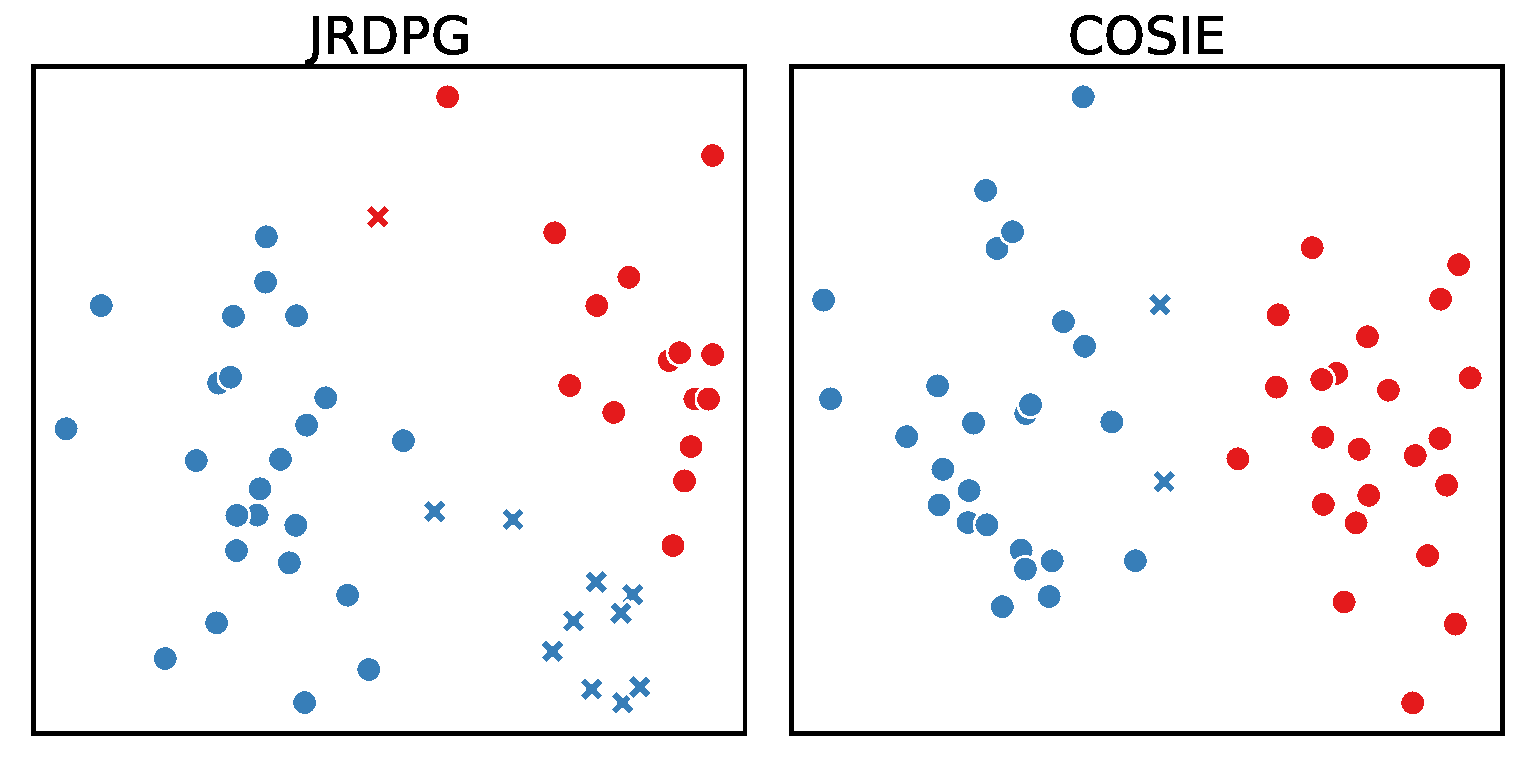
\includegraphics[width=0.65\textwidth]{figures/dnd/exp3_latent_positions.pdf}
%     \caption{\textbf{Visualization of vertices in 2D space in $\jrdpg$ and $\cosie$ models.} Total of $m=100$ $\mathsf{kidney-egg}$ $\sbm$ with $a=0.5$ and $b=0.65$ are sampled. The networks are embedded into $d =2$ dimensions, and the mean estimated latent position matrix, $\bar{\X}$, and the estimated vertex subspace matrix, $\hat{\V}$, are shown. The colors corresponds to the estimated community assignments obtained from 2-cluster $\gmm$. Dots represent correctly labeled vertices and $x$ markers represent incorrectly labeled vertices. As effect size increases, the separation between two communities increase, and misclassification rate decreases.}
%     \label{fig:exp3_latent_positions} % TODO must define 'effect size' here, or not use the term.
%     % TODO: would it be possible to put the embedding for different sizes of graphs to see the effect of increasing n? If it is too much work, I think it is fine, but the plot doesn't look  obviously clustered, so maybe showing that increasing n makes the points to be closer to its mean will be more informative
% \end{figure}

\subsubsection{Seeded Graph Matching (SGM)} \label{sec:sgm}
Consider two graphs $\mathcal{G}^{(1)}$ and  $\mathcal{G}^{(2)}$ with $n$ vertices and their associated adjacency matrices $\A$ and $\B$, respectively. The graph matching problem seeks to find an alignment of nodes between these two graphs that minimizes the number of edge disagreements. Formally, it is defined as the following optimization problem:
% TODONE the below formalization is obtuse.  use the norm formulation like i did in FAQ please, || A - Q B Q\T ||
% TODO we already used P above, so let's use Q for permutation matrix?
\begin{align}
    \min & %{\ \text{-trace}({\A}\Pbf\B^\top \Pbf^\top)} 
    ~\norm*{\A\Pbf - \Pbf\B}_F^2
    \label{eq:GMP}\\
    \mbox{s.t.} & {~\Pbf  \in \mathcal{P}} \nonumber
\end{align}
where $\mathcal{P}$ is the set of permutation matrices in $\RR^{n \times n}$.
% TODONE i think sgm is a modification of GM, not the algorithm FAQ which solves GM.  
Seeded graph matching ($\sgm$) is a modification of the graph matching algorithm, allowing for the specification of seed sets $W_1$, $W_2$ with seeding $\psi : W_1 \rightarrow W_2$, and solved via fast approximate quadratic assignment ($\sct{FAQ}$) \cite{vogelstein2015fast}.
As the seeded graph matching problem is computationally intractable, $\sgm$ provides an approximate solution by relaxing the feasible region from $\mathcal{P}$ to $\mathcal{D}$, the set of doubly stochastic matrices. The algorithm is provided below:
\begin{enumerate}
    \item Initialize at some $\Pbf^{(0)} \in \mathcal{D}$, where $\mathcal{D}$ is the set of doubly stochastic matrices. Typically, initialization is chosen as $\Pbf^{(0)} = \vec{1}\vec{1}^\top / n$, where $\vec{1}$ denotes the $n$-vector of all ones.
    \item \textbf{while} stopping criteria not met \textbf{do}
        \begin{enumerate}
            \item Compute the gradient $\Delta f\left(\Pbf^{(i)}\right)$
            \item Compute the search direction $\Q^{(i)} \in \argmax{\left(\trace{\Q^{T} \Delta f(\Pbf^{\left(i\right)})}\right)}$ via Hungarian Algorithm
            \item  Compute step size $\alpha^{(i)} \in \argmax(f(\alpha^{(i)} \Pbf^{(i)} + (1 - \alpha^{(i)}) \Q^{(i)})) $
            \item Update $\Pbf^{(i+1)} := \alpha^{(i)} \Pbf^{(i)} + (1 - \alpha^{(i)}) \Q^{(i)}$
        \end{enumerate}
    \item Compute $\hat{\Pbf} \in \argmax\left(\trace{\Pbf^{\top} \Pbf^{(final)}}\right)$ via Hungarian Algorithm
\end{enumerate} 

% 7. theory
%     1. single graph theory
%         a. "you say i say"
%         b. central limit theorem for ase/lse
%     2. multi graph theory 
%         a. mase/omni
%         c. nonpar + semipar theory
%         d. sgm correlated-SBM/ER theory

\section{Theory for Statistical Models}
In this section, we provide general outlines of the theorems and proofs for statistical models in Section \ref{sec:models} and algorithms in Section \ref{sec:algorithms}.

\subsection{Theory for Single Graph Models}\label{sec:theory_single}

Graph features, such as the ones described in Section~\ref{sec:bag-of-features}, are popularly used to test hypothesis about a graph. However,  the distribution of such features is usually unknown, and even in cases where the asymptotic distribution is available, one needs to proceed with caution as some of the asymptotic results might be misleading \cite{priebe2010you}.  \cite{Rukhin2010} studies the behavior of two simple graph features, namely, the number of edges and the maximum  degree, for testing a simple hypothesis question about the distribution of a graph. While the statistic based on the number of edges achieves a higher power in the limit as the number of vertices grows, a comparative power analysis shows that even for large graphs with $n\leq 10^{24}$, the statistic based on the maximum degree dominates under certain cases.

A body of existing results in statistical inference for spectral embeddings is reviewed more deeply in \cite{athreya2017statistical}. We summarize next some of the main results related to the exposition in this paper. 
In this section, we assume that a sequence of random adjacency  matrices $\{\A_n, n\geq 1\}$ generated from a sequence of latent positions $\{\X_n, n\geq 1\}$, where  $\A_n\sim \rdpg(\X_n)$, $n\geq 1$ is the adjacency matrix of a graph with $n$ vertices, and $\X_n\in\RR^{n\times d}$ are $d$-dimensional latent positions. We write $(\X_n)_i$ to represent the $i$-th row of $\X_n$, and we assume that the rows of $\X_n$, which correspond to the latent positions, are an i.i.d. sample $(\X_1), \ldots, (\X_n)_n\overset{\text{i.i.d.}}{\sim} F$, where $F$ is a distribution with support $\mathcal{X}\subset\RR^d$. We also  assume that the second moment matrix $\mathbf{\Delta} = \mathbb{E}[(\X_n)_1(\X_n)_1^\top]\in\Real^{d\times d}$, has non-zero eigenvalues.   We use $\widehat{\X}_n=\ase(\A_n)\in\Real^{n\times d}$ to denote the $d$-dimensional adjacency spectral embedding of $\A_n$, and $\widetilde{\X}_n = \lse(\A_n)$  to denote its $d$-dimensional Laplacian spectral embedding.


The adjacency spectral embedding ($\ase$) method described in Section~\ref{sec:ase} is a consistent and asymptotically normal estimator for the latent positions of a random dot product graph. In \cite{sussman2012consistent}, it is shown that clustering rows of the $\ase$ of $\A_n$ can consistently recover the communities of an $\sbm$. Consistency of the latent positions for an $\rdpg$ is studied in  \cite{Sussman2014-zq,Lyzinski2014-pe,Lyzinski2017-cq}. In particular, Theorem 5 of  \cite{Lyzinski2017-cq} shows that with probability tending to one, there exists some orthogonal rotation $\W_n\in\Real^{d\times d}$ such that 
\begin{equation*}
    \max_{i\in[n]}\|(\widehat{\X}_n)_i - \W_n(\X_n)_i\| \leq \frac{Cd^{1/2}\log^2 n}{\sqrt{n}}, \label{eq:thm-ASE-const}
\end{equation*}
where $C>0$ is a constant, and hence, the rows of of $\hat{\X}_n$ converge to the rows of $\X_n$, up to some orthogonal rotation, as the number of vertices $n$ grows. 


Distributional results on the rows of the adjacency spectral embedding show that the error in estimating the true latent positions is asymptotically normally distributed. In particular \cite{Athreya2016} showed  a central limit theorem for the rows of the $\ase$ of $\A_n$, in which the latent positions are shown to converge to a mixture of standard multivariate normal distributions, that is, for any $\mathbf{z}\in\RR^{d}$,
\begin{equation}
   \lim_{n\rightarrow\infty} \mathbb{P}\left(\sqrt{n}\left(\widehat{\X}_n\W_n - \X\right)_i\leq \mathbf{z} \right) = \int_{\mathcal{X}}\Phi(\mathbf{z}, \mathbf{\Sigma}(\mathbf{x}))\  dF(\mathbf{x}),\label{eq:thm-ASE-CLT}
\end{equation}
where $\Phi(\mathbf{z}, \mathbf{\Sigma}(\mathbf{x}))$ is the cumulative distribution function of a multivariate normal distribution with mean zero and a covariance matrix $\mathbf{\Sigma}(\mathbf{x})\in\Real^{d\times d}$ that is a function of $\mathbf{x}\in\mathcal{X}$ (see \cite{Athreya2016}, Theorem 1, for an expression of this covariance matrix). 

Similar results to the ones presented above are also available for the Laplacian spectral embedding ($\lse$). In particular, Theorem 3.1 of \cite{tang2018limit} provides an an asymptotic result on the estimation error of the rows of $\widetilde{\X}_n$  with respect to its population version, and Theorem 3.2 shows an analogous result to the one presented in Equation~\eqref{eq:thm-ASE-CLT} to establish the asymptotic normality of the rows of this estimator, that is,
\begin{equation*}
   \lim_{n\rightarrow\infty} \mathbb{P}\left\{\sqrt{n}\left(\W_n(\widetilde{\X}_n)_i - \frac{(\X_n)_i}{\sqrt{\sum_{j}(\X_n)_i^\top (\X_n)_j }} \right)\leq \mathbf{z}\right\}  = \int_{\mathcal{X}}\Phi(\mathbf{z}, \widetilde{\mathbf{\Sigma}}(\mathbf{x}))\  dF(\mathbf{x}),\label{eq:thm-LSE-CLT}
\end{equation*}
for some covariance matrix $\widetilde{\mathbf{\Sigma}}(\mathbf{x})$ which its exact form is presented in \cite{tang2018limit}.

The consistency and asymptotic normality of  $\ase$ and $\lse$ considered in this section  have been recently extended to the $\grdpg$ model  (see Theorems 5-8 in  \cite{rubin2017statistical}). 



\subsection{Theory for Multiple Graph Models}

\subsubsection{Spectral Embeddings}\label{sec:theory_multi}

The results discussed before have been used to develop valid statistical tests for   two-graph hypothesis testing questions. The work of \cite{tang2017semiparametric} studies a semiparametric graph hypothesis testing for the equivalence between the latent positions of the vertices of a pair of graphs. Formally, for each fixed $n$ let $\X_n, \Y_n\in\Real^{n\times d}$ be a sequence of latent positions matrices, and define
$\A_n\sim\rdpg(\X_n)$, $\B_n\sim\rdpg(Y_n)$ as independent random adjacency matrices. The problem of testing the equality of the distributions of $\A_n$ and $\B_n$  is defined as
\begin{equation*}
    \mathcal{H}^n_0:\X_n =_{\W} \Y_n\quad\quad\quad \text{ vs.}\quad\quad\quad \mathcal{H}^n_a:\X_n \neq_{\W} \Y_n,
\end{equation*}
where $\X_n =_{\W}\Y_n$ denotes that $\X_n$ and $\Y_n$ are equivalent up to an orthogonal transformation $\W\in\mathcal{O}_d$, and $\mathcal{O}_d$ is the set of $d\times d$ orthogonal matrices. To define the test statistic, denote  $\widehat{\X}_n = \ase(\A_n)$, $\widehat{\Y}_n=\ase(\B_n)$, and for a matrix $\A\in\Real^{n\times n}$ with singular values $\sigma_1(\A) \geq \ldots\geq \sigma_n(\A)\geq 0$ and largest observed degree $\delta(\A) = \max_{i\in[n]}\sum_{j=1}^n\A_{ij}$, define 
$$\gamma(\A):=\frac{\sigma_d(\A) - \sigma_{d+1}(\A)}{\delta(\A)}.$$ 
Define $T_n$ as the test statistic
\begin{equation*}
    T_n : = \frac{\min_{\W\in\mathcal{O}_d} \|\widehat{\X}_n\W - \widehat{\Y}_n\|_F}{\sqrt{d\gamma^{-1}(\A_n)} + \sqrt{d\gamma^{-1}(\B_n)}}.
\end{equation*}
It is shown in Theorem 3.1 of \cite{tang2017semiparametric} that  $T_n$ is a consistent test for the  hypothesis testing problem described above, in the sense that for any significance level $\alpha$ and $C>1$, then  $\mathbb{P}(T_n> C)\leq \alpha$ for $n$ sufficiently large under $\mathcal{H}^n_0$ (type I error control), and if $\lim_{n\rightarrow\infty}\min_{\W\in\mathcal{O}_d} \|\widehat{\X}_n\W - \widehat{\Y}_n\|_F=\infty$, then $\mathbb{P}(T_n> C)\rightarrow 1$ under $\mathcal{H}^n_a$ (i.e., the type II error vanishes). For specific assumptions and some extensions to other hypothesis testing problems, the reader is referred to \cite{tang2017semiparametric} and \cite{athreya2017statistical}.

When the vertices of the graphs are not necessarily aligned (including cases in which the graphs do not have the same number of vertices), testing equality of latent positions is inappropriate. The work of \cite{tang2017nonparametric} proposes a nonparametric test to determine whether the distribution of the latent positions of the graphs is the same. For a pair of matrices $\X_n\in\Real^{n\times d}$ and $\Y_m\in\real^{m\times d}$ with their rows distributed as $(\X_n)_i\overset{\text{i.i.d.}}{\sim} F$ and $(\Y_m)_i\overset{\text{i.i.d.}}{\sim} G$ and a pair of independent adjacency matrices $\A_n\sim\rdpg(\X_n)$, $\B_n\sim\rdpg(\Y_n)$ , the nonparametric graph hypothesis testing problem is given by
\begin{equation*}
    \mathcal{H}^n_0:F \upVdash G \quad\quad\quad \text{ vs.}\quad\quad\quad \mathcal{H}^n_a: F \nupVdash G,
\end{equation*}
where $F\upVdash G$ indicates equality of the distributions up to an orthogonal transformation. To test such hypothesis, \cite{tang2017nonparametric} proposes to use the following test statistic
\begin{align*}
    U_{n,m}(\X, \Y)=& \frac{1}{n(n-1)}\sum_{j\neq i}\kappa(X_i, X_j)-\frac{2}{mn}\sum_{i=1}^n\sum_{k=1}^m\kappa(X_i, Y_k)\\
    & + \frac{1}{m(m-1)}\sum_{l\neq k}\kappa(Y_k, Y_l),
\end{align*}
where $\kappa:\mathcal{X}\times \mathcal{X}\rightarrow\Real$ is a positive definite kernel. In \cite{tang2017nonparametric}, Theorem 1, it is shown that $U_{n,m}(\X, \Y)$ is a consistent and unbiased estimate of the maximum mean discrepancy \cite{gretton2012kernel} between the distributions $F$ and $G$. Furthermore, under the null hypothesis, the quantity $(m+n)U_{n,m}(\X, \Y)$ converges in distribution to an infinite weighted sum of independent chi-squared random variables as $n,m\rightarrow \infty$, provided that $\frac{n}{n+m}\rightarrow \rho \in (0, 1)$.  Moreover, when the latent positions are used in place of the true latent positions, then Theorem 4 of \cite{tang2017nonparametric} shows that the difference between $U_{n,m}(\widehat{\X}, \widehat{\Y})$  and $U_{n,m}(\X, Y)$ converges to zero sufficiently fast to yield a consistent test procedure.

% Under the null hypothesis that $F = G$ (up to some orthogonal transformations), 
% \begin{equation*}
%     (m+n)(U_{n,m}(\widehat{\X}, \widehat{\Y}) - U_{n,m}({\X}, {\Y}\W_{n,m})) \overset{a.s.}{\rightarrow} 0.
% \end{equation*}
% Under the alternative hypothesis, 
% \begin{equation*}
%     \frac{(m+n)}{\log^2(m+n)}(U_{n,m}(\widehat{\X}, \widehat{\Y}) - U_{n,m}({\X}, {\Y}\W_{n,m})) \overset{a.s.}{\rightarrow} 0
% \end{equation*}

% Suppose that $n,m\rightarrow\infty$ and $\frac{m}{m+n}\rightarrow\rho\in(0,1)$.

%Theorem 43 of \cite{athreya2017statistical} (consistency of nonpar)

The work of \cite{levin2017central} studies the omnibus embedding described in Section~\ref{sec:omni} under the joint random dot product graph ($\jrdpg$) model, where $(\A^{(1)}, \ldots, \A^{(m)})\sim\jrdpg(\X_n)$, and the rows of $\X_n\in\Real^{n\times d}$ are an i.i.d. sample from some distribution $F$. Let $\widehat{\mathbf{O}}\in\Real^{mn\times mn}$ be the omnibus embedding of $\A^{(1)}, \ldots, \A^{(m)}$ and $\widehat{\Z} = \ase(\mathbf{O})\in\Real^{mn\times d}$.
Under this setting, it is shown in Lemma 1 of \cite{levin2017central} that the rows of $\widehat{\Z}_n$ are a consistent estimator of the latent positions of each individual graph  as $n\rightarrow\infty$, and that
\begin{equation}
\max_{i\in[n],j\in[m]}\|(\widehat{\Z}_n)_{(j-1)n + i} - \W_n(\X_n)_{i}\| \leq \frac{C\sqrt{m}\log(mn)}{\sqrt{n}}. \label{eq:OMNI-consistency}    
\end{equation}
Furthermore, a central limit theorem for the rows of the omnibus embedding  asserts that
\begin{equation}
   \lim_{n\rightarrow\infty} \mathbb{P}\left\{\sqrt{n}\left(\W_n(\widehat{\Z}_n)_{(j-1)n + i} - (\X_n)_i\right)\leq \mathbf{z}\right\}  = \int_{\mathcal{X}}\Phi(\mathbf{z}, \widehat{\mathbf{\Sigma}}(\mathbf{x}))\  dF(\mathbf{x}),\label{eq:thm-OMNI-CLT}
\end{equation}
for some covariance matrix $\widehat{\Sigma}(\mathbf{x})$ (see Theorem 1 of \cite{levin2017central} for an exact expression). In recent work, \cite{draves2020bias} extended the study of the omnibus embedding and provided results analogous to the ones in Equations~\eqref{eq:OMNI-consistency} and \eqref{eq:thm-OMNI-CLT} under a more general model that allows for differences in the latent positions of each graph.


The $\cosie$ model described in Section~\ref{sec:cosie} describes multiple networks with expected probability matrices that share the same common invariant subspace. It is shown in \cite{arroyo2019inference} that the $\mase$ algorithm (see Section~\ref{sec:mase}) is a consistent estimator for this common invariant subspace, and produces asymptotically normally distributed estimates for the individual symmetric matrices. Specifically, let $\V_n\in\Real^{n\times d}$ be
a sequence of orthonormal matrices and $\R^{(1)}_n, \ldots, \R^{(m)}_n\in\Real^{d\times d}$ a sequence of score matrices such that $\mathbf{P}^{(l)}_n=\V_n\R^{(l)}_n\V_n^\top\in[0,1]^{n\times n} $, $(\A_n^{(1)}, \ldots, \A_n^{(m)})\sim \cosie(\V_n;, \R^{(1)}_n, \ldots, \R^{(m)}_n)$, and $\widehat{\V}, \widehat{\R}^{(1)}_n, \ldots, \widehat{\R}^{(1)}_n$ be the estimators obtained by $\mase$. Under appropriate regularity conditions (see Theorem 3 of \cite{arroyo2019inference}), the estimate for $\V$ is consistent as $n,m\rightarrow\infty$, and there exists some constant $C>0$ such that
        \begin{equation*}
			\mathbb{E}\left[\min_{\W\in\mathcal{O}_d}\|\widehat{\V}-\V\W\|_F\right] \leq C\left(\sqrt{\frac{1}{mn}} + {\frac{1}{n}}\right). \label{eq:theorem-bound}
		\end{equation*}
    In addition, the entries of $\widehat{\mathbf{R}}^{(l)}_n$, $l\in[m]$ are asymptotically normally distributed. Namely, there exists a sequence of orthogonal matrices $\W$ such that
		$$\frac{1}{\sigma_{l,j,k}}\left(\widehat{\R}^{(l)}_n - \W^\top\R^{(l)}_n\W + \Hmat_m^{(l)}\right)_{jk} \overset{d}{\rightarrow} \mathcal{N}(0, 1), $$
		as $n\rightarrow\infty$, where
		$\mathbb{E}[\|\Hmat_m^{(l)}\|]=O\left(\frac{d}{\sqrt{m}}\right)$ and $\sigma^2_{l,j,k} = O(1)$. 
		For a  precise statement about the joint distribution of the entries of $\widehat{\mathbf{R}}_n^{(i)}$, see Theorem 7 in \cite{arroyo2019inference}.


\subsubsection{Graph Matching for Correlated Networks } Given a pair of graphs $\A_n$ and $\B_n$ with $n$ vertices each, the graph matching problem tries to find a correspondence between their vertices. A body of literature has studied the feasibility of finding the correct matching under different random graph models, including correlated  Erd\H{o}s-R\'enyi  \cite{Lyzinski2013-fq,cullina2016improved} and Bernoulli graphs
\cite{lyzinski2015graph}. In this section we review some of the results for the correlated Erd\H{o}s-R\'enyi model described in Section~\ref{sec:correlated-graphs}.

Formally, given parameters $\rho_n\in[0,1]$ and $q_n \in(0, 1-\xi_1)$ for some small $\xi_1>0$, the $n\times n$ adjacency matrices $\A_n$ and $\B_n$ are distributed as correlated Erd\H{o}s-R\'enyi if their marginal distributions are $\A_n\sim\er_n(q_n)$, $\B_n\sim\er_n(q_n)$, but the edge pairs satisfy $\text{Corr}((\A_n)_{ij},(\mathbf{Q}_n^\top\B_n\mathbf{Q}_n)_{ij})=\rho_n$, where $\mathbf{Q}_n\in\mathcal{P}_n$ is a permutation matrix that gives the correct alignment between the vertices (here $\mathcal{P}_n$ denotes the set of $n\times n$ permutation matrices). The work of \cite{Lyzinski2013-fq}  studies the feasibility of finding $\mathbf{Q}_n$ by solving the optimization problem defined in Equation~\eqref{eq:GMP}. In particular, it is shown that there exists positive constants $c_1, c_2$ such that if $\rho_n\geq c_1\sqrt{\frac{\log n}{n}}$ and $q_n\geq c_2 \frac{\log n }{n}$, then $\mathbf{Q}_n$ can be correctly recovered  with probability 1 for $n$ sufficiently large (Theorem 1 of \cite{Lyzinski2013-fq}). 

While the solution of the quadratic assignment problem \eqref{eq:GMP} can correctly recover the vertex alignment in theory, it is computationally challenging to solve the optimization problem. In the presence of $s_n$ seed vertices with known correspondence between the graphs, \cite{Lyzinski2013-fq} introduced an efficient polynomial algorithm to recover the alignment of the remaining $n-s_n$ vertices.
Theorem 2 of \cite{Lyzinski2013-fq} shows that this method can correctly recover $\mathbf{Q}_n$ in the setting where $\xi_2 < p_n<1-\xi_2<1$ and $\xi_2 < \rho_n < \xi_2$ for some $\xi_2>0$ in the presence of a logarithmic number of seeds (i.e. $s_n\geq c_3 \log n$ for some $c_3>0$).
\section{Data Descriptions}
The following two datasets are analyzed using the algorithms and models described Sections \ref{sec:models} and \ref{sec:algorithms}. Section \ref{sec:single_app} primarily focuses on the \textit{Drosphila} connectome, while Section \ref{sec:multi_app} primarily focuses on HCP connectomes.

\subsection{\textit{Drosphila} Larval Mushroom Body Data Description}\label{sec:drosphila}
The connectome was estimated from serial-section electron microscopy (EM) of an L1 \textit{Drosophila} larva \cite{eichler2017complete}. For the mushroom body (MB) subcircuit, the graph was defined by manually identifying synapses in the EM volume, and tracing the pre- and post-synaptic partners through the EM volume back to their cell bodies. Each node in this graph represents an individual neuron, and each edge consists of one or more synapses between those neurons. Thus, edge weights are the number of synapses between neurons. 

Each node in the graph also has an associated cell type: Kenyon cell (KC), projection neuron (PN), MB input neuron (MBIN), and MB output neuron (MBON). Additionally, we can categorize neurons based on hemisphere (which side of the brain each neuron was on), and neuron pair (for most neurons, a homologous pair neuron in the other hemisphere was identified by morphological comparison).

\subsection{HCP Data Description}\label{sec:hcp}
We used publicly available diffusion MRI (dMRI) and structural MRI (sMRI) data from the S1200 (2017) release of the Human Connectome Project (HCP) Young Adult study, acquired by the Washington University in St. Louis (WUSTL) and the University of Minnesota (Minn) \cite{hcp1, hcp2}. Out of the 1206 participants released, 1059 had viable dMRI for processing. 

Connectomes were estimated using the ndmg pipeline \cite{Kiar188706}. Briefly, the dMRI scans were pre-processed for eddy currents using FSL's \texttt{eddy-correct} \cite{fsl1}. FSL's ``standard" linear registration pipeline was used to register the sMRI and dMRI images to the MNI152 atlas \cite{fsl1,fsl2,fsl3,mni152}.A tensor model is fit using DiPy \cite{dipy} to obtain an estimated tensor at each voxel. A deterministic tractography algorithm is applied using DiPy's EuDX \cite{dipy,eudx} to obtain streamlines, which indicate the voxels connected by an axonal fiber tract. We used a modified version of Desikan–Killiany–Tourville (DKT) parcellation \cite{DKT}  to define the ROIs. Graphs are formed by counting the number of fibers between a pair of ROIs. 

% TODONE seems like drosophila is only in 6, and HCP is only in 7? if so, you can absorb this section into the appropriate subsections. 
% TODO@jv - not quite true since the graph matching is in multi-graphs
\section{Applications for Single Graph Data}\label{sec:single_app}
In this section, we explore the applications of the single graph models in Section \ref{sec:single_graph_models} and the algorithms in Section \ref{sec:single_algo}. The \textit{Drosophila} mushroom body connectome and HCP data are analyzed (see Appendix \ref{sec:drosphila} and \ref{sec:hcp} for description) along with simulated examples, and Appendix \ref{sec:single_app_appendix} contain additional analysis in weighted connectomes. 

\subsection{Testing for Differences Between Communities of Edges}
\label{sec:sg_dros_siem}

In Figure \ref{fig:siem_uwt}, we compare a number of different strategies using Fisher's exact test \cite{fisher1925statistical} for testing whether there exists a difference between $K=2$ communities, or groups, of edges in a graph. Formally, let $e_{ij}^{(k)} \sim F_k$ be a single edge in the graph, where $k \in\left\{ 1, 2\right\}$ is a community of edges, for $i, j \in [n]$. Our hypothesis test of interest is:
\begin{align*}
    H_0: F_1 = F_2, \quad
    H_a: F_1 \neq F_2
\end{align*}
We simulate graphs from the homophilic planted partition $\sbm$  from Section \ref{sec:usbm} and symmetric homotopic $\siem$ from Section \ref{sec:usiem} in Figure \ref{fig:siem_uwt}a(i). Under the given models, our hypotheses simplify to testing whether $p_1 = p_2$ against $p_1 \neq p_2$; that is, whether or not there exists a different probability for each edge community. Effect size, or the difference in probability between the two communities, for the $\sbm$ and the $\siem$ are varied linearly from $0$ to $0.1$, and from $0$ to $0.5$, respectively. 
% Under the null, the distributions $F_1, F_2$ of the two communities are identical, and under the alternative, the two distributions are different. 
A relative effect size of $0$ corresponds to an $\er$ graph, in which $F_1 = F_2$; at all other relative effect sizes, the alternative is true. We measure performance using the statistical power at $\alpha = 0.05$ in Figure \ref{fig:siem_uwt}a(ii). Across the simulation settings, we see that Fisher's exact test provides an appropriate statistical test and provides sufficiently high  power with large enough effect size and graph. Importantly, Fisher's test displays  both empirical validity (at an effect size of zero, the power is at most $\alpha$) and empirical consistency (the test power converges to $1$ as the effect size increases) in both simulations.

We demonstrate our techniques developed above on the \textit{Drosophila} mushroom body, with $n=319$ vertices in the left or right hemisphere (2 vertices located along the center of the brain are excluded). In Figure \ref{fig:siem_uwt}b we investigate the appropriateness of different unweighted independent edge models for the \textit{Drosophila} mushroom body. Our goal is to identify whether the unweighted \textit{Drosophila} mushroom body display homophilia (that is, the within hemisphere blocks have greater connectivity than between hemisphere blocks) or homotopia (that is, edges incident bilateral vertices have a different distribution from edges incident non-bilateral vertices). Figure \ref{fig:siem_uwt}b(i) shows the unweighted \textit{Drosophila} mushroom body. The within-hemisphere blocks appear to have a higher proportion of edges than the between-hemisphere edge blocks, shown in Figure \ref{fig:siem_uwt}b(ii). There is strong evidence that the within-hemisphere connectivity exceeds the between-hemisphere connectivity (Fisher's exact test, $p$-value=$0.0$). Next, we investigate whether the graph is homotopic; that is, whether bilateral (homotopic) connectivity exceeds non-bilateral (heterotopic) connectivity, in Figure \ref{fig:siem_uwt}b(iii). Strong evidence is present that homotopic connectivity exceeds heterotopic connectivity (Fisher's exact test, $p$-value=$0.0$).

Finally, we explore the appropriateness of various independent edge models for diffusion connectomes from the HCP Dataset. The diffusion connectomes are binarized according to whether an edge is present (the edge weight is greater than zero) or absent (the edge weight is zero). Figure \ref{fig:siem_uwt}c(i) shows the average unweighted diffusion connectome over all participants in the study. Figure \ref{fig:siem_uwt}c(ii) shows the distribution of edge-weights within-hemisphere versus between-hemisphere. The diffusion connectomes appear to possess homophily; i.e., high within-hemisphere connectivity, with lower between-hemisphere connectivity. This is demonstrated by the fact that in all $N$=$1059$, the within-hemisphere connectivity exceeds the between-hemisphere connectivity. This effect can be observed by looking at the difference between within-hemisphere connectivity and between-hemisphere connectivity for each of the $N=1059$ connectomes, shown in \ref{fig:siem_uwt}c(iii). All $1059$ diffusion connectomes have significantly higher within-hemisphere connectivity than between-hemisphere connectivity at $\alpha=.05$ after Bonferroni correction (Fisher's exact test, $N=1059$, maximum $p$-value$<10^{-20}$).

\begin{figure}
    \centering
    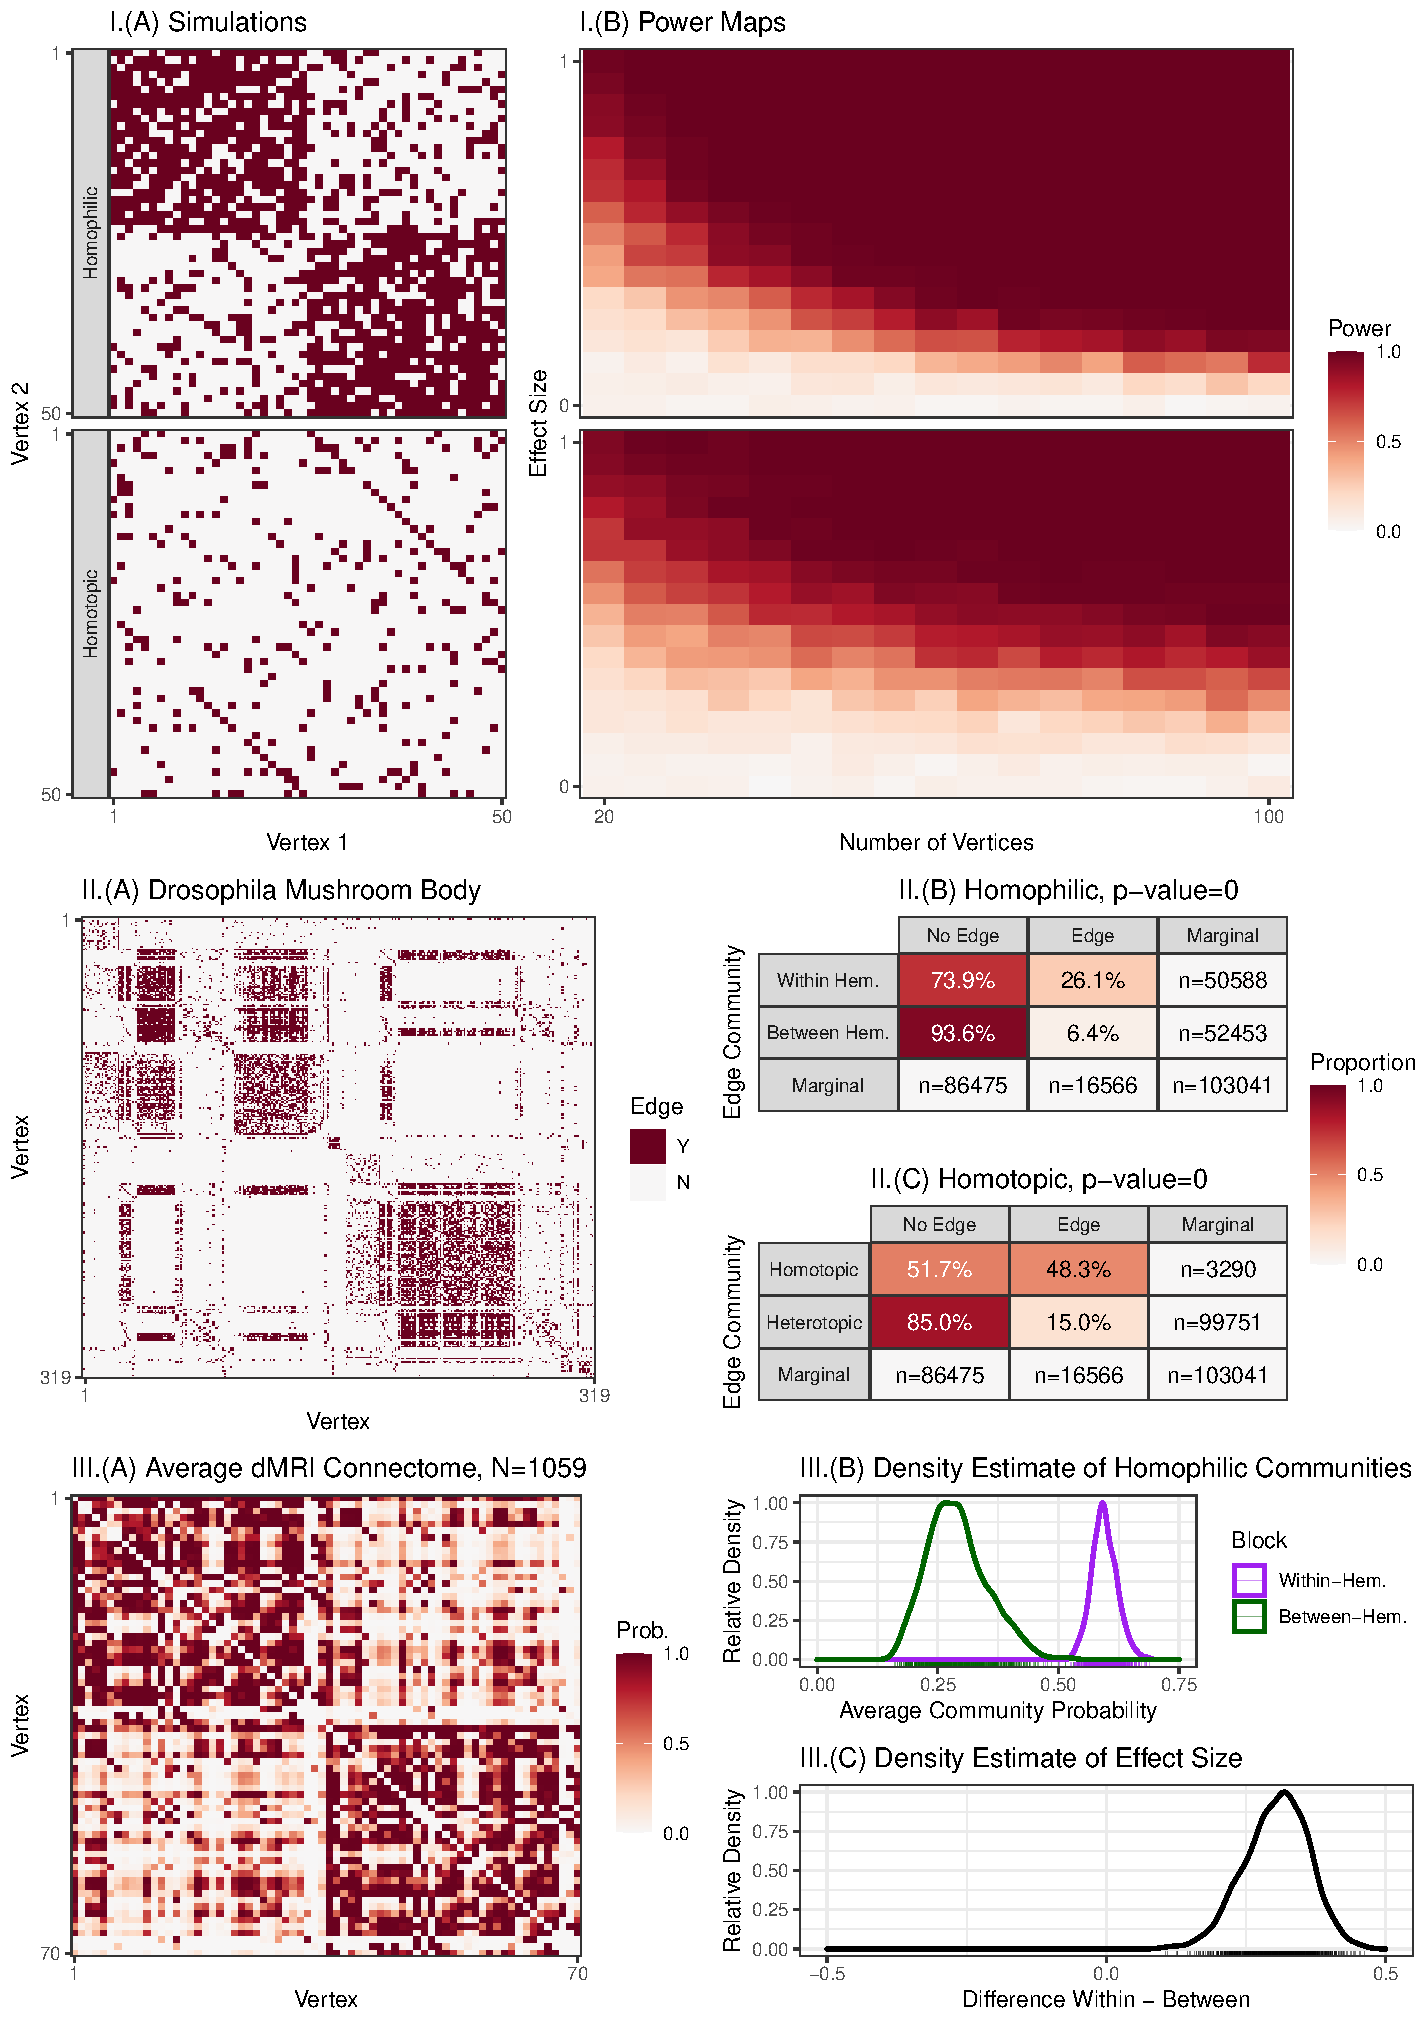
\includegraphics[width=.9\linewidth]{figures/dnd/siem_figure.pdf}
    \caption
    [Comparing communities of edges in graphs.]
    {\textbf{Comparing communities of edges in graphs}. \textbf{a(ii)} Fisher's exact test shows reasonable statistical power across both homophilic and homotopic block structures in \textbf{a(i)}, with power converging to $1$ as effect size and number of vertices grow. \textbf{b(ii)} and \textbf{b(iii)} the \textit{Drosophila} mushroom body in \textbf{b(i)} shows both homophilic planted partition and homotopic structure (Fisher's exact test, $p$-values$=0$). \textbf{c(ii)} and \textbf{c(iii)} all $N=1059$ Human Connectome Project (HCP) diffusion connectomes show homophilic planted partition structure, with within-hemisphere connectivity exceeding between-hemisphere connectivity (Fisher's exact test, $N=1059$, Bonferroni corrected $p$-values$<10^{-21}$).}
    \label{fig:siem_uwt}
\end{figure}

Appendix \ref{sec:siem_wt} investigates the fit of independent edge models for weighted graphs from the \textit{Drosophila} mushroom body and the HCP diffusion connectomes. We leverage the Mann-Whitney Wilcoxon Test, a non-parametric test of whether there exists a difference in medians between the two edge-clusters. We again find that the weighted \textit{Drosophila} mushroom shows both homotopic planted partition structure and homophily, and that the weighted HCP connectomes all show homotopic planted partition structure ($N$=$1059$), a conclusion consistent with our results on the unweighted graphs. 

\subsection{Model Selection for Appropriate Block Structure}
\label{sec:sbm_block_est}

Recall that in Section \ref{sec:usbm}, that for the case of a $K=2$ $\sbm$, the matrix $\B$ with entries $\B_{kl}$ defines the probability of an edge connecting a vertex in community $k$ with a vertex in community $l$. By the bias-variance trade-off, simply supposing a unique entry for each block of $\B$ adds an additional level of complexity to the model, and may reduce the quality of inference, so the ability to make a principled decision when faced with numerous potential block structures is of importance. Formally, we are concerned with choosing one of the appropriate block structures from a subset of candidate block structures given in Section\ref{sec:usbm}, presenting a problem in model selection. Our hypotheses are the alternate candidate models, and our goal is to select the hypothesis corresponding to the candidate model that is most supported by the data by using the model with the lowest $p$-value.

In Figure \ref{fig:sbm_uwt}a, we perform simulations where the true graph is either $\er$, Planted Partition, and Symmetric Heterogeneous, as shown in Figure \ref{fig:sbm_uwt}a(i). Effect size corresponds to the magnitude of the difference between disparate blocks in the model. We find that the $\chi^2$ test 
is an appropriate test for identification of block structure in unweighted graphs, and successfully recovers the correct block structure as the effect size and the number of vertices increases. Figure \ref{fig:sbm_uwt}a(ii) shows the test features both empirical validity and empirical consistency, as in Figure \ref{fig:siem_uwt}. 
% Performance is worst for the Asy. Het. example, when each block has its own unique probability.

In Figure \ref{fig:sbm_uwt}b, we investigate the appropriate block structure for the unweighted \textit{Drosophila} mushroom body, which is shown in  shows the probability of an edge existing within each block of $\B$, where the $n=319$ vertices in either the left or right hemisphere are partitioned according to hemisphere. 
% TODONE 'it would appear'? is this a soap opera? just state the results please ;)
% phantom of the opera actually :D --eb
The on-diagonal (Left,Left) and (Right,Right) blocks share a similar distribution that is unique from the (Left, Right) and (Right, Left) blocks. Because the \textit{Drosophila} mushroom body is inherently a directed graph, we investigate whether it is $\er$, Planted Partition, Asymmetric Homogeneous, Symmetric Heterogeneous, or Asymmetric Heterogeneous, using the $\chi^2$ test. Testing indicates that the \textit{Drosophila} mushroom body possesses a planted partition structure ($\chi^2$ test, $p$-value=$0.0$). 
% TODONE what does 'the best fit model is to assume symmetic ....' mean? maybe state p-values for each test?
This has the interpretation that the optimal $\sbm$ includes a shared probability for the on-diagonal (Left,Left) and (Right,Right) blocks, and a different shared probability for the off-diagonal (Left,Right) and (Right,Left) blocks. An important considerations is that while the optimal $\sbm$ is symmetric, the graph itself is directed. This has the implication that while the $\sbm$ would posit that edges in the (Left,Right) and (Right,Left) blocks have the same probability, realizations of the (Left,Right) and (Right,Left) block will not necessarily be identical. 

Figure \ref{fig:sbm_uwt}c investigates the optimal block structure for the $N$=$1059$ diffusion connectomes from the HCP dataset. The figure shows the average connectivity for the $3$ possible unique entries of the block probability matrix $\B$ for an $\sbm$ where vertices are segmented into communities according to hemisphere: Left-Hemisphere Connectivity, Right-Hemisphere Connectivity, and Contralateral (between-hemisphere) connectivity. Because the diffusion connectomes are inherently symmetric, the graph is directionless, and hence it is not possible for the \textit{Left, Right} and \textit{Right, Left} blocks to have different values. We consider $3$ possible block structures for the diffusion connectome: $\er$, Planted Partition, and Symmetric Heterogeneous. On all $N$=$1059$ connectomes, the optimal block structures is Planted Partition, using the $\chi^2$ test.

Appendix \ref{sec:sbm_est_wt} proposes the use of several testing variants (ANOVA, Kruskal-Wallis, and Distance Correlation) for the weighted drosophila mushroom body and the weighted HCP diffusion connectomes for investigating the optimal block structure. All tests yield the same conclusion (and in the case of the HCP dataset, again for all $N$=$1059$ connectomes) that the mushroom body and diffusion connectomes display planted partition structure. An important consideration is that the implication for weighted graphs is, rather than the on-diagonal and off-diagonal blocks sharing the same probability (as is the case for the unweighted graphs), the 2 on-diagonal blocks (\textit{Left, Left} and \textit{Right, Right}) share a \textit{common distribution}. The implication is similar for the 2 off-diagonal blocks (\textit{Left, Right} and \textit{Right, Left}).

\begin{figure}
    \centering
    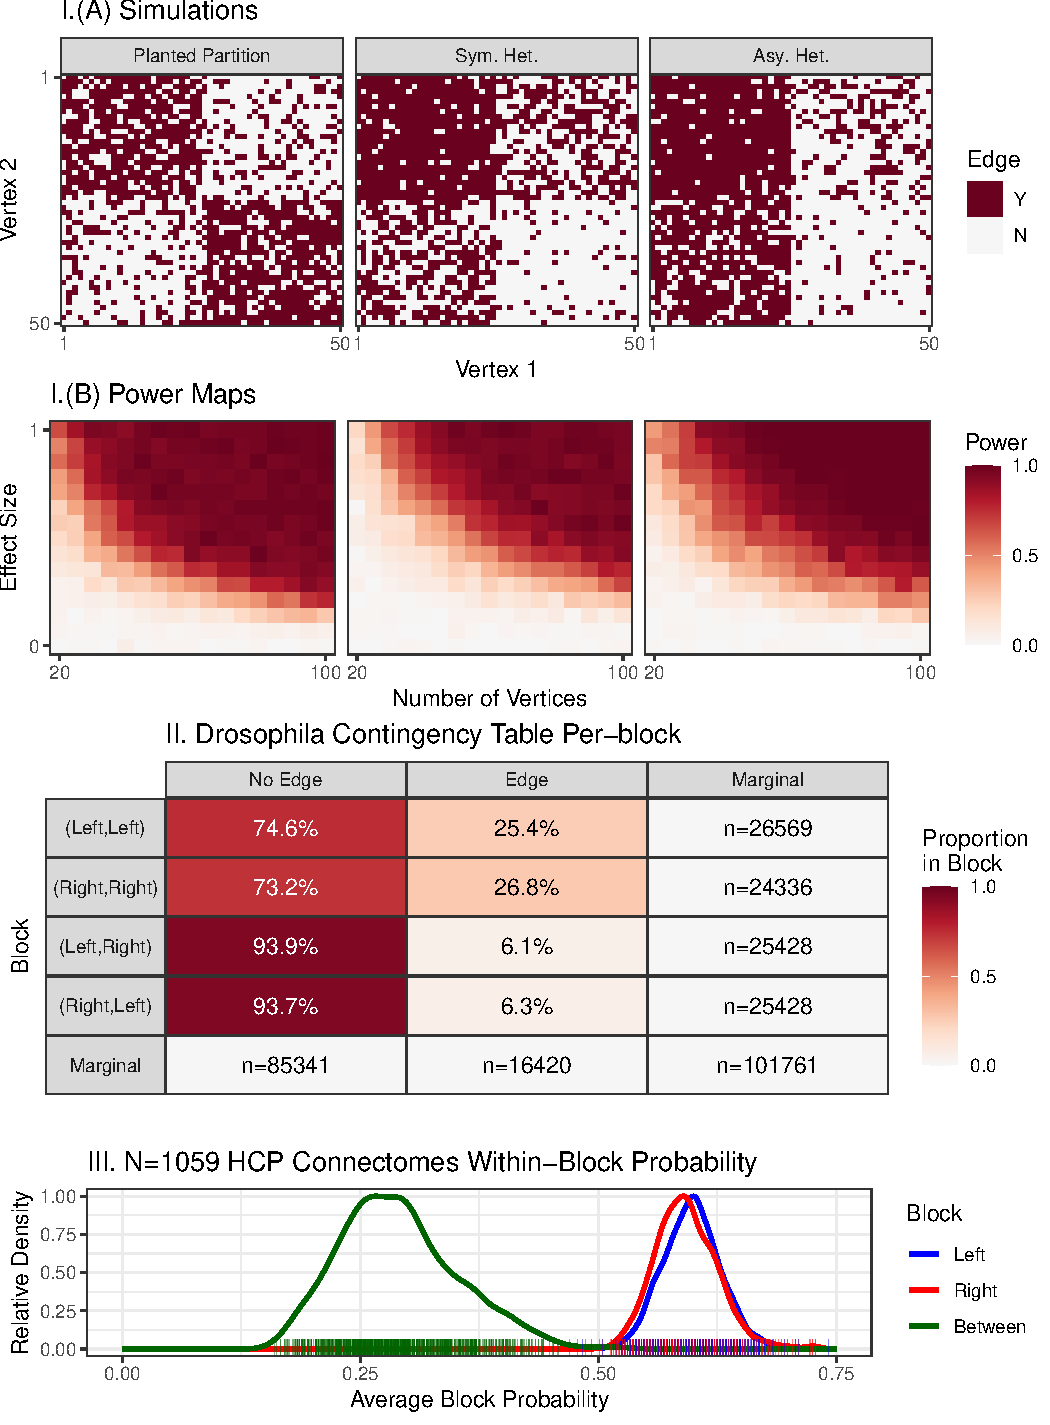
\includegraphics[width=.8\linewidth]{figures/dnd/sbm_uwt.pdf}
    \caption
    [Estimating optimal block structure.]
    {\textbf{Estimating optimal block structure}. \textbf{a(ii)} $\chi^2$ test is effective for identifying the ideal block structure across disparate candidate block structures from \textbf{a(i)}, as power improves as both effect size and graph size increase. \textbf{b.} The \textit{Drosophila} mushroom body displays a planted partition structure ($\chi^2$ test, $p$-value=$0.0$), where \textit{(Left, Left)} and \textit{(Right, Right)} blocks share a different probability from the \textit{(Left, Right)} and \textit{(Right, Left)} blocks. \textbf{c.} Similarly, all $N=1059$ Human Connectome Project (HCP) diffusion connectomes show planted partition structure, with a similar interpretation to the \textit{Drosophila} result.}
    \label{fig:sbm_uwt}
\end{figure}


\subsection{Same Network, Different Communities}
In the case of 2-block $\sbm$s with positive semi-definite block probability matrix $\B = [a, b;b,c]$, there are two structures of interest: affinity and core-periphery. In affinity structure, $a, c \gg b$, that is the within-block connectivity is relatively higher than that of between-block connectivity. In the core-periphery structure, $a \gg b, c$, that is one block has relatively higher within-block connectivity than those of other block's within-block probability and between-block connectivity.

In this section, we examine the two spectral embedding clustering approaches described in Section \ref{sec:ase} which produce different clusterings depending on the $\sbm$ model \cite{priebe2019two, cape2019spectral}. In short, $\ase$ clustering tends to favor core-periphery structure while $\lse$ clustering tends to favor affinity structure.

We consider graphs generated from 4-block $\sbm$ with $n=4000$ vertices, membership vector $\vec{\pi} = [0.25, 0.25, 0.25, 0.25]$, and the block probability matrix
\begin{align*}
    \mathbf{B} = 
    \begin{blockarray}{ccccc}
        & A & B & C & D \\
        \begin{block}{c[cccc]}
        A & 0.01 & 0.02  & 0.01   & 0.002 \\
        B & 0.02 & 0.1   & 0.002  & 0.015  \\
        C & 0.01 & 0.002 & 0.01  & 0.02 \\
        D & 0.002 & 0.015 & 0.02 & 0.01 \\
        \end{block}
    \end{blockarray}
\end{align*}
The above 4-block $\sbm$ exhibit both affinity and core-periphery structures when projected down to 2-blocks, which are shown below:
\begin{align*}
    \mathbf{B}_{affinity} \approx 
    \begin{blockarray}{ccc}
        & AB & CD  \\
        \begin{block}{c[cc]}
        AB & 0.04 & 0.007  \\
        CD & 0.007 & 0.04  \\
        \end{block}
    \end{blockarray},~ &
    \mathbf{B}_{core} \approx
    \begin{blockarray}{ccc}
        & AC & BD  \\
        \begin{block}{c[cc]}
        AC & 0.01 & 0.01  \\
        BD & 0.01 & 0.06  \\
        \end{block}
    \end{blockarray}
\end{align*} 
Blocks $AB$ and $CD$ form $B_{affinity}$, which exhibit the affinity structure, while blocks $AC$ and $BD$ form $B_{core}$, which exhibit the core-periphery structure. 
A network is sampled from the 4-block $\sbm$ model, and spectral clustering is performed (see Section \ref{sec:clustering_single}) with embedding dimension $\hat d=2$ and $K=2$ number of clusters. Figure \ref{fig:exp8} shows the spectral clustering results. In panel \ref{fig:exp8}a, clustering with $\lse$ shows the blocks forming affinity structures are grouped together, and, in panel \ref{fig:exp8}b, clustering with $\ase$ shows the blocks forming core-periphery structures grouped together. Thus, the two different spectral clustering methods provide two different groups that are both meaningful. 

\begin{figure}
    \centering
    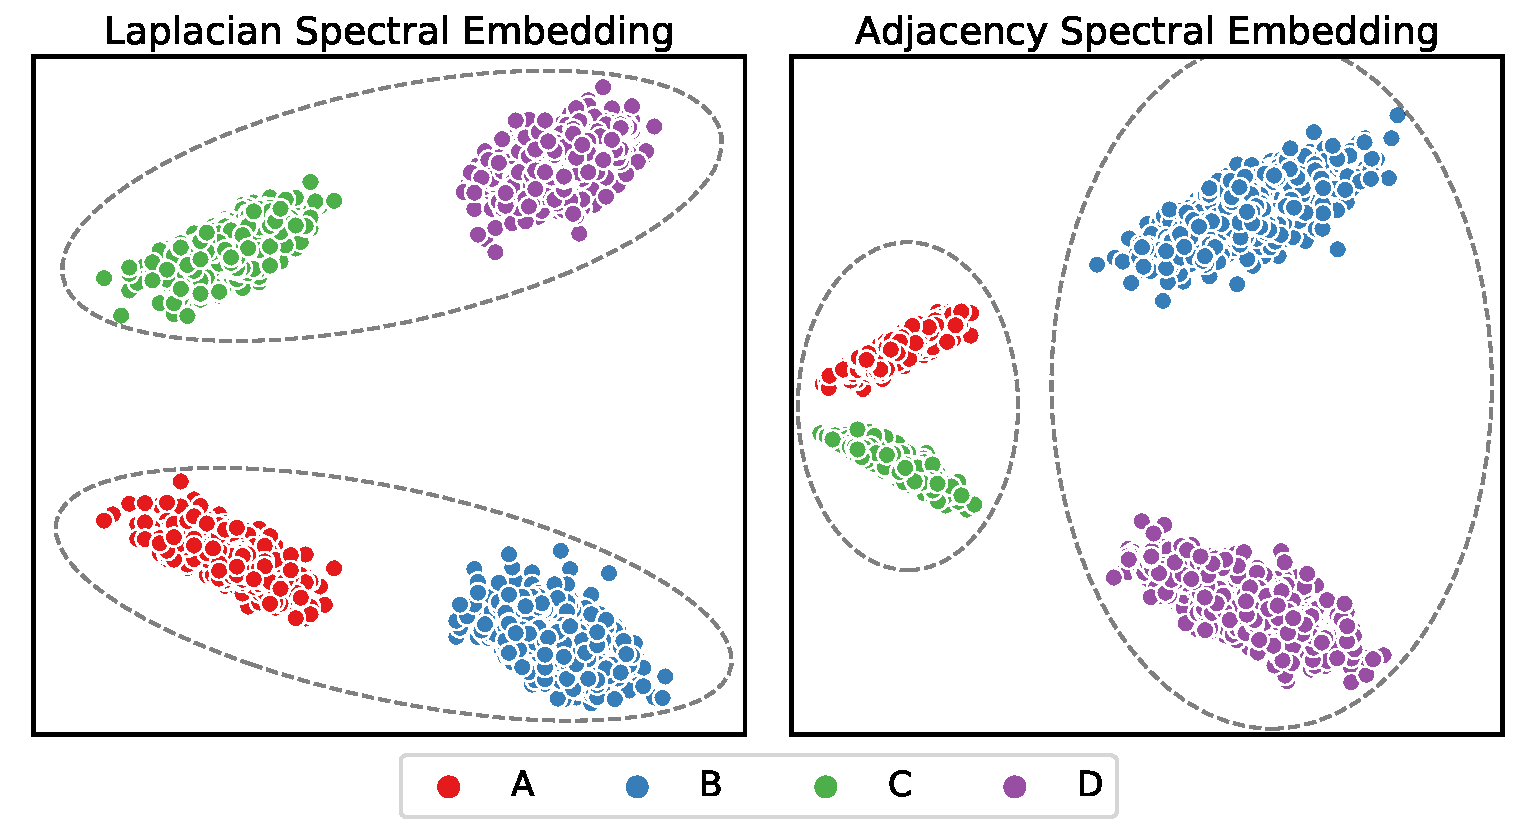
\includegraphics[width=0.7\textwidth]{figures/dnd/two_truths}
    \caption
    [Different clustering results from adjacency spectral embedding ($\ase$) and Laplacian spectral embedding ($\lse$).]
    {\textbf{Different clustering results from adjacency spectral embedding ($\ase$) and Laplacian spectral embedding ($\lse$).} For both $\ase$ and $\lse$, the network was embedded into $d=2$ dimensions, and Gaussian mixture modelling ($\gmm$) with $K=2$ clusters were fit. The dots represent vertices in the embedded space and the colors correspond to block memberships. The dashed black ellipses define the vertices that were clustered into same group.
    \textbf{a.} Clustering the embeddings from $\lse$ results in affinity clustering. 
    \textbf{b.} Clustering the embeddings from $\ase$ results in core-periphery clustering.}
    \label{fig:exp8}
\end{figure}

\subsection{Detecting Communities with Spectral Clustering}
Many of the techniques described above rely on knowing an \textit{a priori} grouping of nodes or edges, but in many real-world examples this information is not available. Additionally, one may seek to discover communities in the network, either for modeling the network as a block-model or to reveal groups of similar nodes. 

As described in Section \ref{sec:clustering_single}, one can embed a graph via $\ase$ or $\lse$ and then use $\gmm$ to reveal communities of nodes. Here, we separately embed both the left and right hemisphere induced subgraphs of the \textit{Drosophila} larva connectome using $\ase$ (see \cite{priebe2017semiparametric} for an extensive investigation) with $\hat d= 3$. $\gmm$ was performed independently on both hemispheres, with the clustering assignments and embeddings shown in Figure \ref{fig:mb-clustering}. Note that while the embedding and clustering of both hemispheres were performed separately, similar structures emerge for the left and right. In particular, each cluster is mostly comprised of a single cell type. Thus, spectral clustering can provide neuroscientists to find meaningful communities when the assignment is not known. 

\begin{figure}
    \centering
    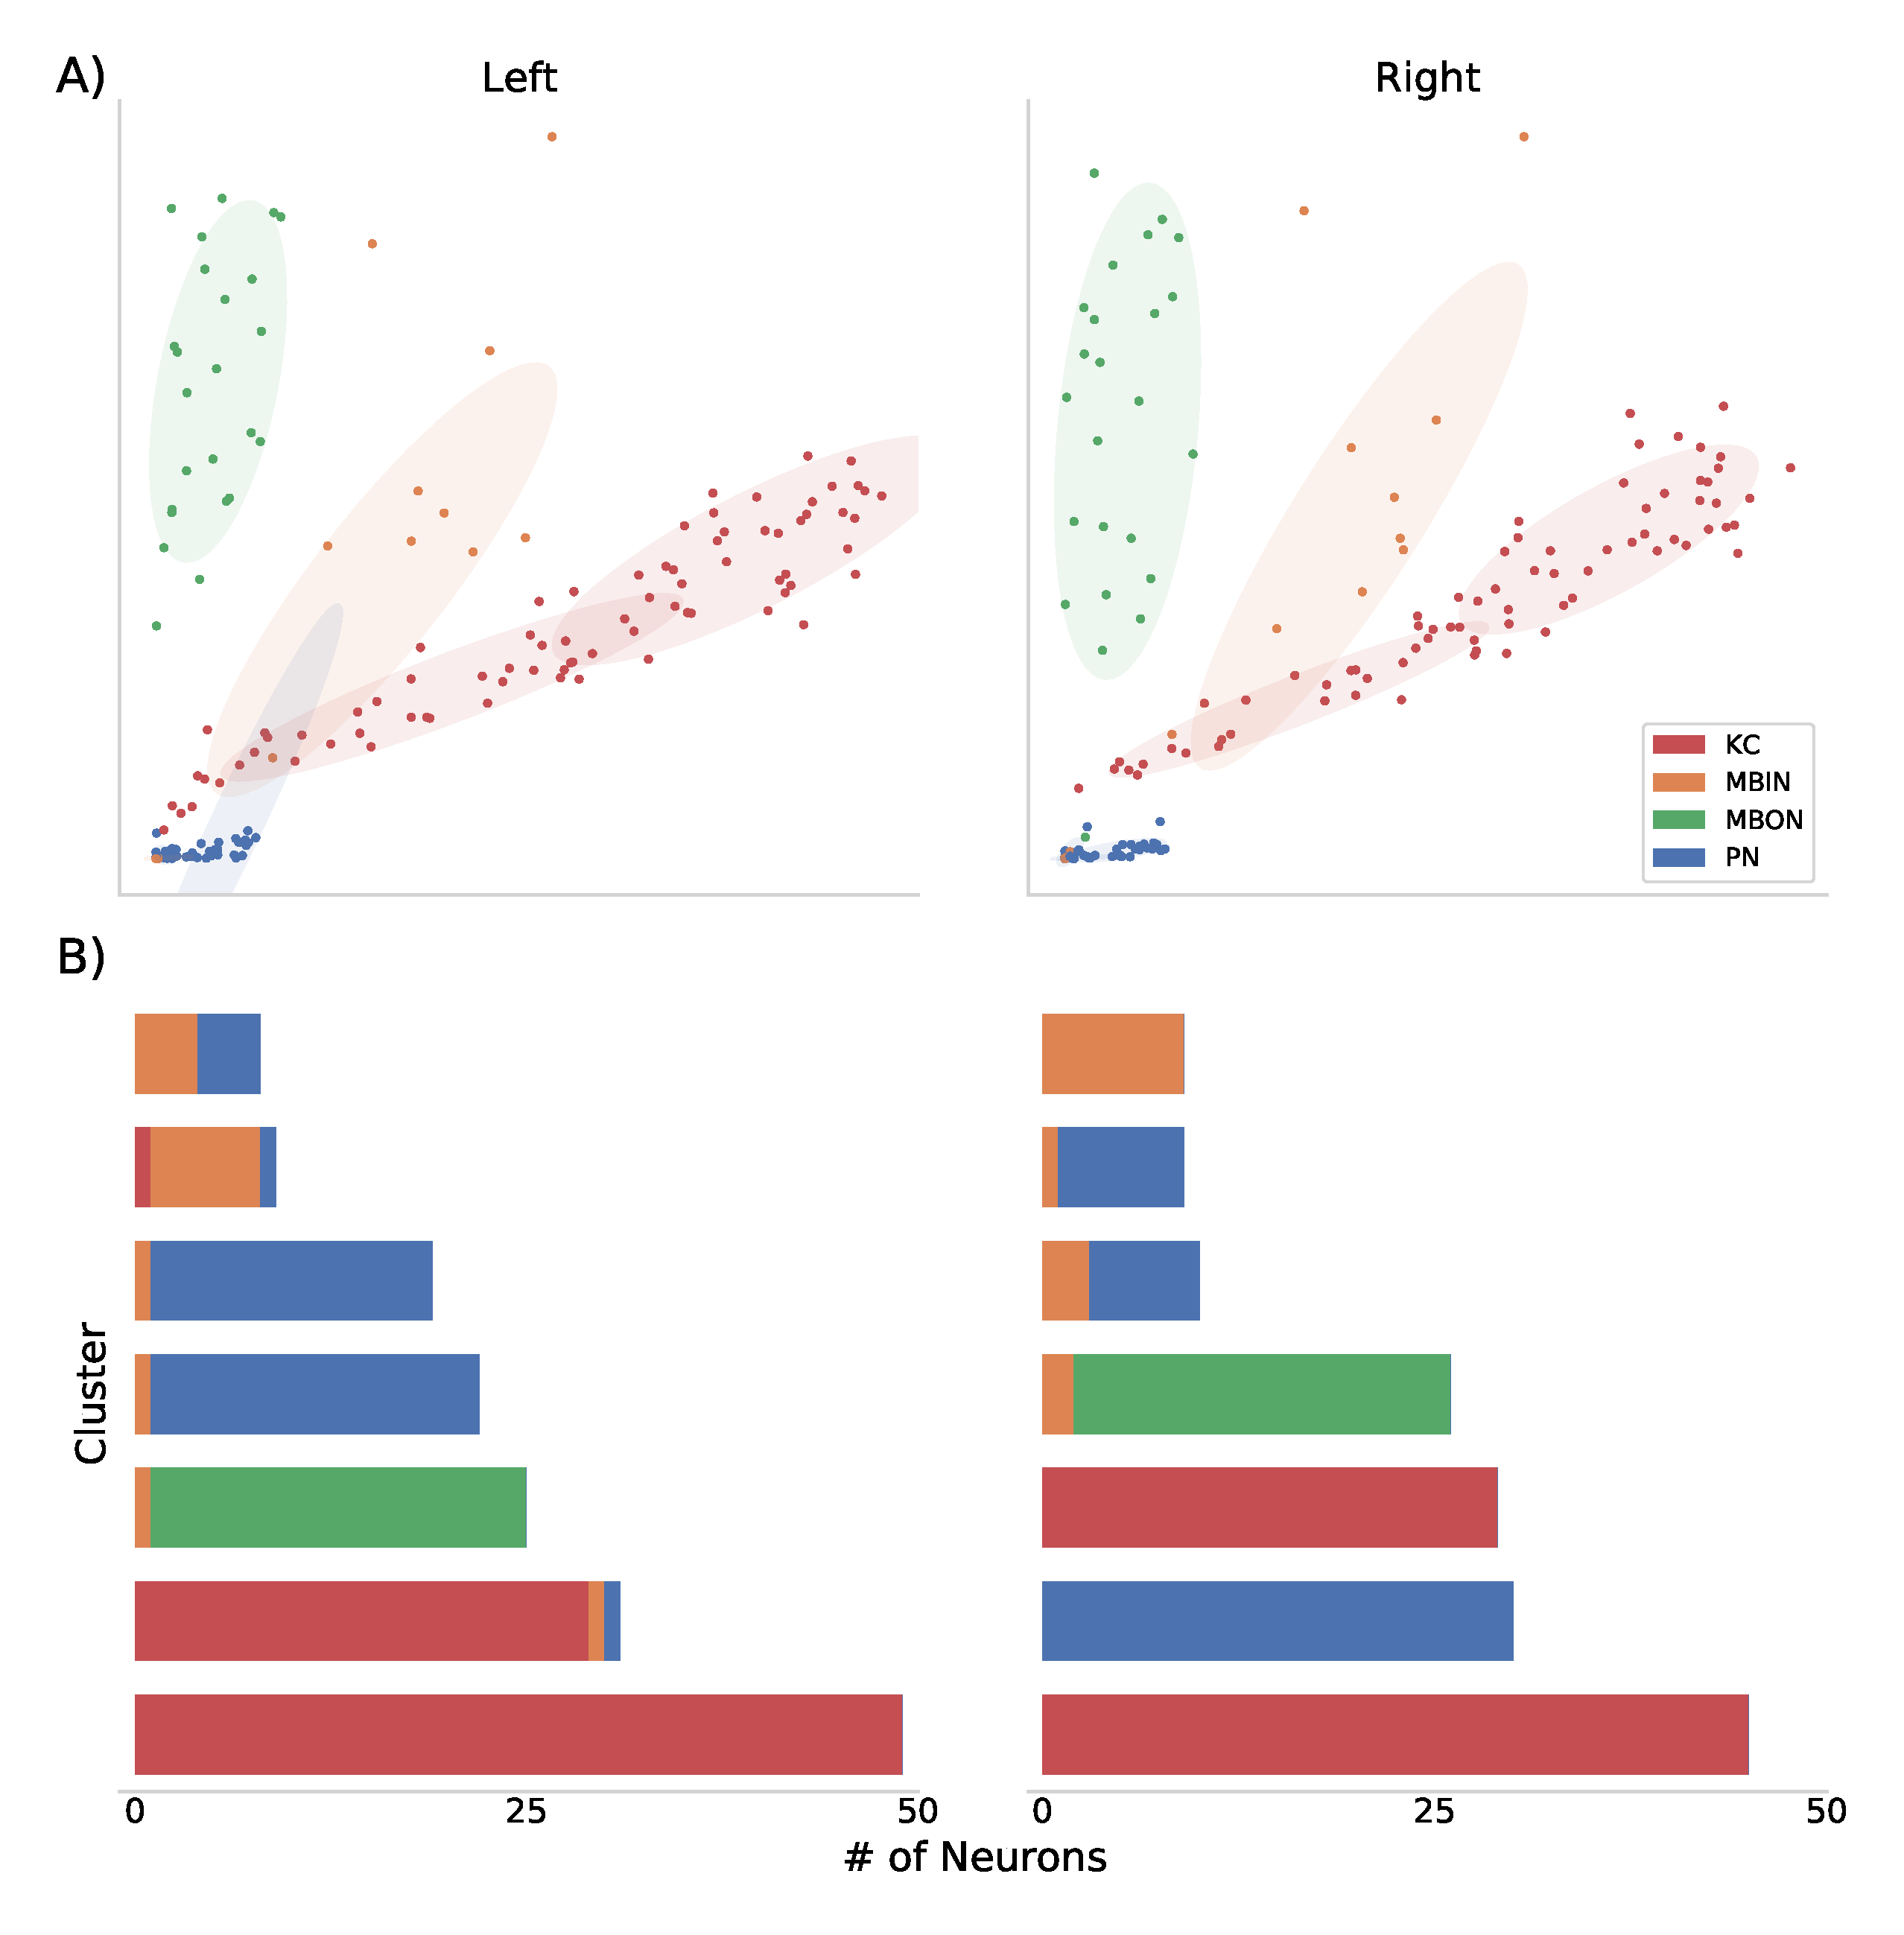
\includegraphics[width = .8\linewidth]{figures/dnd/mb-clustering.pdf}
    \caption
    [Spectral clustering of the \textit{Drosophila} mushroom body network.]
    {\textbf{Spectral clustering of the \textit{Drosophila} mushroom body network.} \textbf{a.} First ``in'' embedding dimension is plotted against the first ``out'' embedding dimension for both the left and right hemisphere networks (note that the clustering was performed in six dimensions, but only two are shown here for visualization). Each point represents a neuron, colored by its corresponding cell type. Ellipses show the clusters predicted by Gaussian mixture modeling, colored according to the cell type with the most frequent neurons in that cluster. Each color corresponds to one of Kenyon cells, input neurons, output neurons, and projection neurons. \textbf{b.} Stacked barplots showing each cluster's composition in terms of neuron cell type, for both the left and the right hemisphere clusterings. Each cluster is mostly comprised of a single cell type for both left and right hemisphere networks, meaning that spectral clustering can recover true communities. }
    \label{fig:mb-clustering}
\end{figure}


\section{Applications for Multi-Graph Data}\label{sec:multi_app}
In this section, we explore the applications of the multiple graph models in Section \ref{sec:multi_graph_models} and the algorithms in Section \ref{sec:multi_algo} using simulated and HCP data. Appendix \ref{sec:multi_app_appendix} contain additional exploration in weighted connectomes. 

\subsection{Matching Vertices between Subgraphs} 
For many statistical approaches on graphs, knowing an alignment or matching between the vertices of one graph and another can be useful. For instance, if each neuron on the left hemisphere of the brain has a corresponding neuron in the right hemisphere, then both hemispheres could be jointly embedded and compared using techniques such as $\omni$ or $\mase$. In the case of the mushroom body network, hemilateral neuron pairs were identified for 198 of the neurons considered in Figure \ref{fig:mb-clustering}, yielding 99 neuron pairs. 

Here, we test the ability of graph matching techniques to identify this structure in an unsupervised manner, based only on the network topology (note that the neuron pairs considered here were based on both topology and morphology). We perform unseeded graph matching
% GM is a problem to solve, FAQ is an algorithm.
between the subset of left and right hemisphere neurons for which pairs are known. We restart the algorithm 256 times, and choose the run with the best objective function value (not matching accuracy). Results are shown in Figure \ref{fig:mb-matching}. This matching correctly identified 78.8\% (78/99) of neuron pairs, and all incorrectly matched neurons were matched to a neuron of the correct cell type.

Given a new connectome, where the correspondence between neurons is not known, this method can provide neuroscientists with a faster and statistically-grounded estimate of neuron pairing. 

\begin{figure}
    \centering
    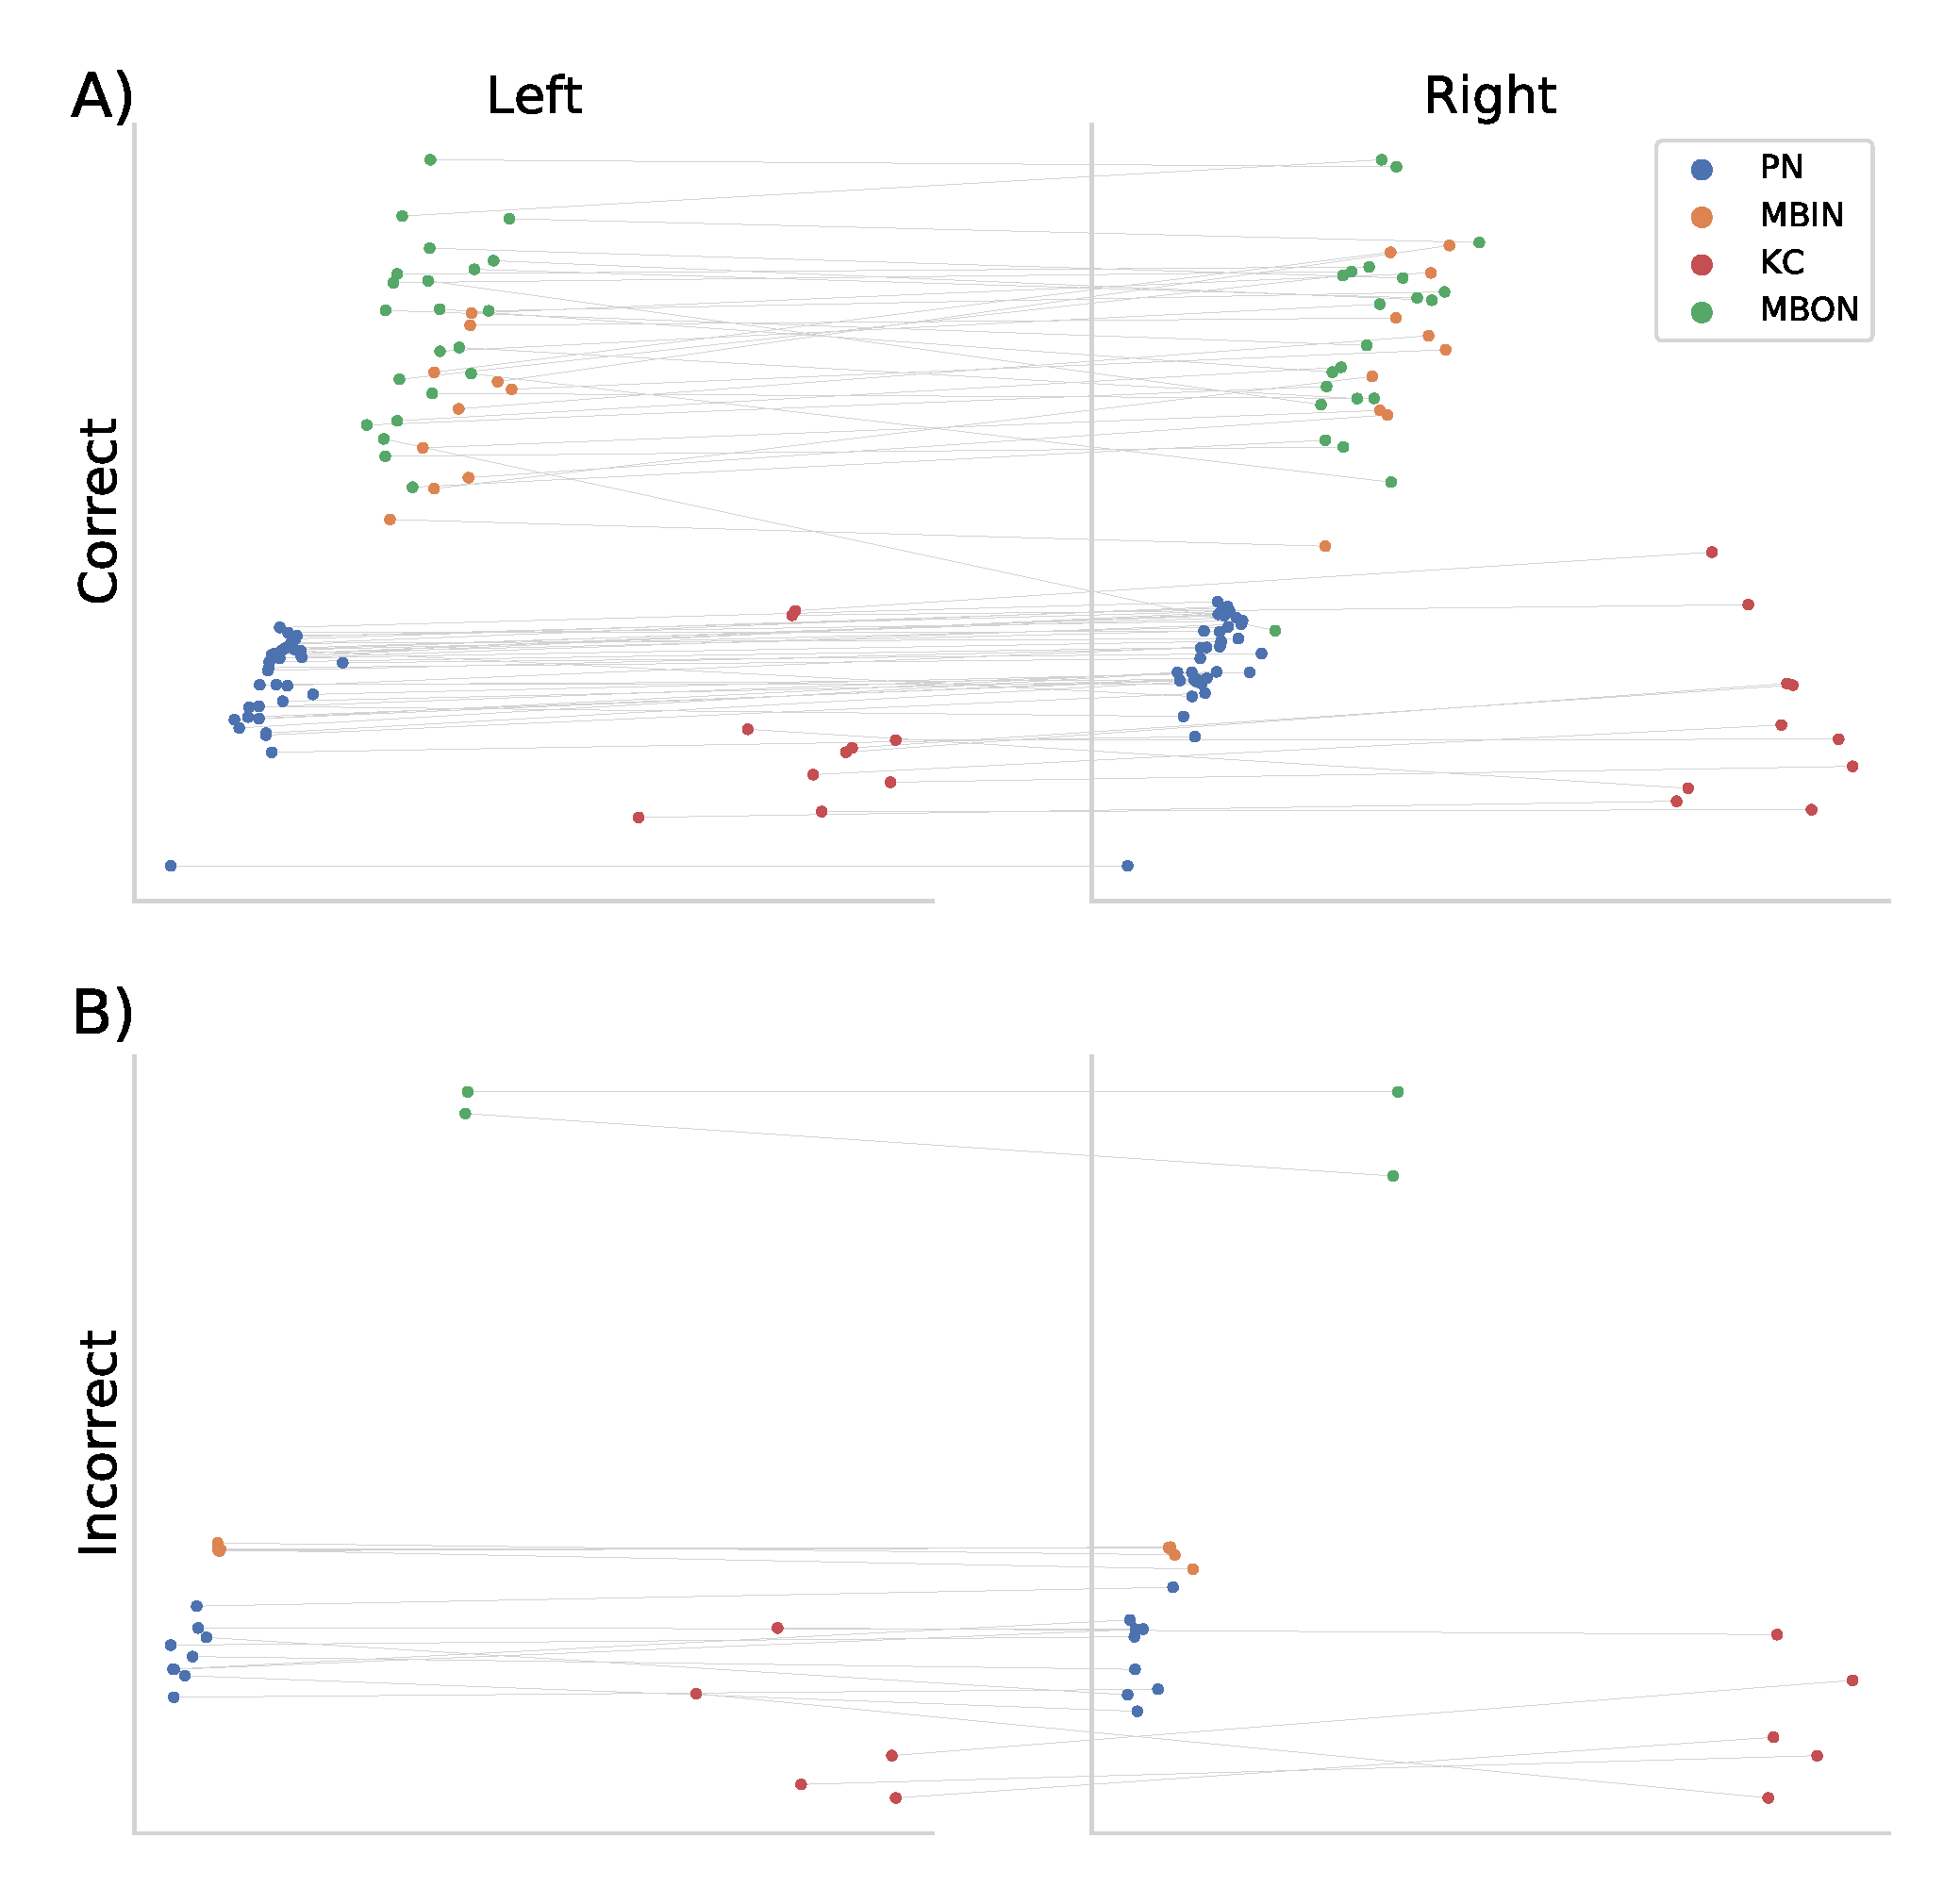
\includegraphics[width = .8\linewidth]{figures/dnd/mb-matching.pdf}
    \caption{\textbf{Graph matching on the \textit{Drosophila} mushroom body network.} All panels show the first two dimensions of principal component analysis $\sct{PCA}$ on the adjacency spectral embedding ($\ase$) of the mushroom body network (for visualization purposes). Each point represents a neuron in the network which has a manually identified pair in the opposite hemisphere, and colors represent one of Kenyon cells, input neurons, output neurons, and projection neurons. 
    Lines show the neuron pair that was predicted by graph matching. 
    \textbf{a.} All of the correctly matched neuron pairs. 78.8\% of neuron pairs (78/99) were correctly matched. 
    \textbf{b.} All of the incorrectly matched neuron pairs. Note that all of the incorrectly matched neurons are matched to neurons of the same cell type.}
    \label{fig:mb-matching}
\end{figure}

\subsection{Testing for Significant Edges} \label{sec:exp1}
We consider two populations of networks generated from an $\er$ model and a 2-block $\mathsf{Kidney-Egg}~\sbm$ model. All networks have $n=20$ vertices and $\pi = \bracks*{0.25, 0.75}$. The block probability matrices for each population is given by $\B^{(1)} = [p, p; p, p]$ and $\B^{(2)} = [p+\delta, p; p, p]$ where $p=0.5$. 
% \begin{align*}
% \B^{(1)} = 
%     \begin{bmatrix}
%     p & p \\ p & p
%     \end{bmatrix},~
% \B^{(2)} = 
%     \begin{bmatrix}
%     p+\delta & p \\ p & p
%     \end{bmatrix}
% \end{align*}
% TODONE should B_11 be bold?
% TODO@jv - yes keeping the bold face even for element of matrix
The difference between the two population is in the first block, $\B_{11}$, and $\delta$ is the magnitude of the difference which ranges from $0$ to $(1-p)$. In other words, $\delta$ is the effect size. Total of $m$ networks are sampled ($\frac{m}{2}$ networks per population). 
For each edge, the t-test test statistics is computed between the two populations, which are then ranked from largest to smallest in magnitude. Ranking of the test statistics and a cutoff is utilized rather than p-value corrections (e.g. Bonferroni) to control for false positive rate. In this case, the ten edges with largest magnitudes are considered since we expect ten edges to be different. 
Non-parametric tests are not considered since many of them are based on ranking the underlying data, which is not sensible for binary data. 
The performance is evaluated with recall@10, which quantifies the fraction of the top ten ranked edges are indeed the truly different edges, averaged over 100 repeated trials.

Figure \ref{fig:exp1}a shows that when the effect size is small ($\delta \leq 0.05$), significant edges cannot be detected even at largest sample sizes ($m=1000$). On the other hand, when effect size is large ($\delta \geq 0.45$), significant edges can be perfectly detected at relatively small sample sizes ($m \geq 30$). 

Connectivity in human brains was analyzed using the structural connectomes (see Appendix \ref{sec:hcp}). For each edge, the class conditional mean, which is the estimated connectivity probability, is computed for females ($m = 572$) and males ($m=488$). The sample sizes and difference in conditional means, which is the estimated effect size, are used to find the closest recall@10 values from the simulated experiment, denoted empirical trustworthiness shown in Figure \ref{fig:exp1})b. Thus, empirical trustworthiness is the confidence in which one can trust that a significant edge is truly significant. There are 2380 possible total edges in connectomes with 70 vertices, but only 49 edges have trustworthiness $\geq 0.9$, meaning one can only trust significance for small set of edges.

\begin{figure}
    \centering
    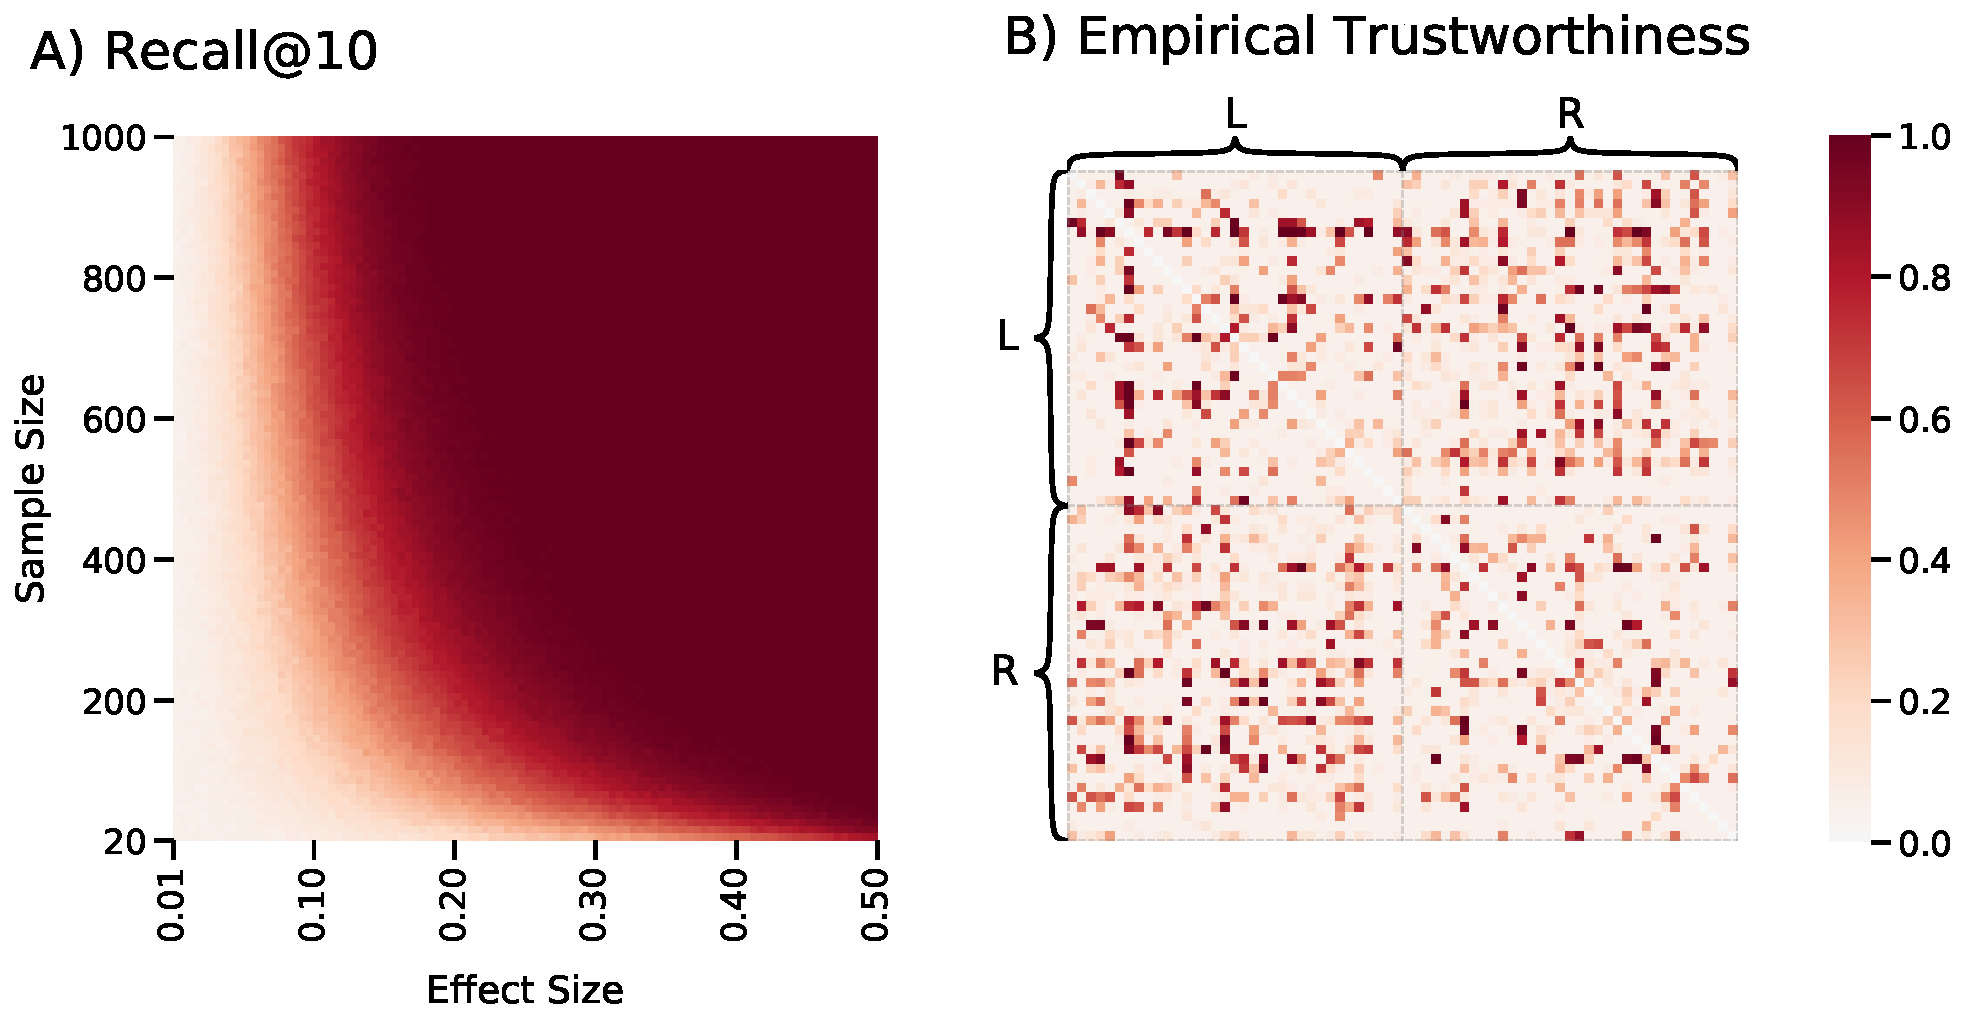
\includegraphics[width=.75\textwidth]{figures/dnd/exp1_final}
    \caption{
    \textbf{Performance of finding significant edges in two different populations of networks.}
    \textbf{a.} Recall for varying sample size and effect size when comparing two populations of binary networks using t-test.
    The color bar represents recall@10 averaged over 100 trials. 
    When effect size is small, significant edges cannot be detected even at large sample size. When effect size is large, significant edges can be detected at small sample sizes ($m=1000$). 
    \textbf{b.} Analysis of structural connectomes from the Human Connectome Project (HCP) data, and the vertices are organized by left (L) and right (R) hemispheres. Edge weights are binarized to parallel the simulations. Heatmap shows the empirical trustworthiness of significant edges when comparing each edge between females and males.}
    \label{fig:exp1}
\end{figure}

Appendix \ref{sec:exp3} investigates the edge-wise testing in weighted connectomes. We leverage the t-test, Mann-Whitney, and Kolmogorov-Smirnov (KS) test, which is a non-parametric test of whether there exists a difference in empirical cumulative distributions between edge weights. We find that KS test is the only test that is appropriate for weighted edges since KS test can detect changes in not only the means, but also changes in variance. In weighted HCP connectomes, we find that 256 edges have trustworthiness $\geq 0.9$, and that very small fraction of edges can be trusted to be significant.



% \begin{summary}[SUMMARY POINTS]
% Depending on the sample size and effect size per edge, one can ascertain the trustworthiness of differences across two populations.
% \end{summary}

% TODO i'd make the adjmat 2x in size, and stack B and C.
% TODO the figure seems to only be about homophylic? why didn't we also do homotopic? can we?
% \begin{figure}
%     \centering
%     \includegraphics[width=\linewidth]{figures/dnd/hcp_siem_uwt.pdf}
%     \caption{\textbf{Goodness of fit of homophilic and homotopic $\siem$ for HCP connectomes}. \textbf{A)} The average unweighted HCP diffusion connectome across $N$=$1059$ connectomes, where connectomes are binarized according to whether the weight is greater than zero or equal to zero. Vertices are arranged according to hemisphere. \textbf{(B)} A density estimate of the average community probabilities across all $N$=$1059$ connectomes. Hashes on the x-axis indicate the observed average probability in the respective block, for each connectome within the dataset (a total of $N=1059$ hashes for each block).  \textbf{(C)} A density estimate of the difference in average within-hemisphere connectivity and average between-hemisphere connectivity for all $N$=$1059$ connectomes. In all connectomes, within-hemisphere connectivity exceeds between-hemisphere connectivity (Fisher's exact test, $N$=$1059$, maximum $p$-value$<10^{-20}$) after Bonferroni correction.}
%     \label{fig:hcp_siem_uwt}
% \end{figure}

% TODO i think i'd intergrate these things into single graph section.  figs 14 & 15 are just studying many connectomes, it is not leveraging multi-graph models in any sense, so it belongs in the single graph section.  also will make things easier for ready, as we can have 1 figure for homotopy/homophyly, instead of the 3 we currently have, distributed throughout (keeping all the panels, just moving content around).
%TODO i would say graph matching doesn't leverage multi-grpah models either and its in here since it makes more sense to be here.

% \begin{figure}
%     \centering
%     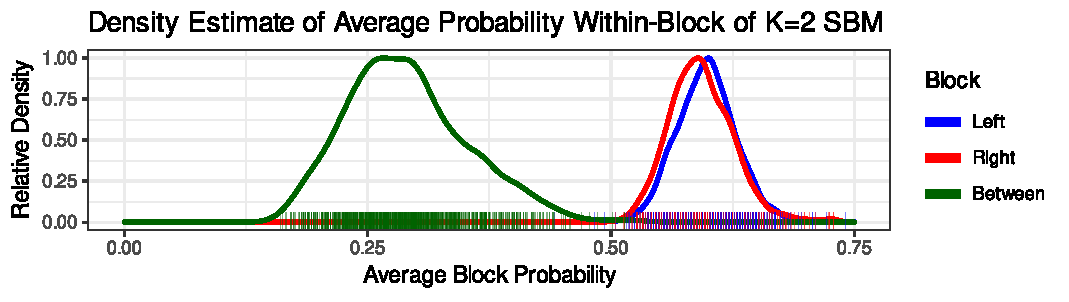
\includegraphics[width=.9\linewidth]{figures/dnd/hcp_block_est_uwt.pdf}
%     \caption{\textbf{Optimal block structure for HCP diffusion connectomes}. We investigate the optimal block structure for the $N$=$1059$ HCP Diffusion Connectomes, where the connectomes are binarized as in Figure \ref{fig:hcp_siem_uwt}. For each connectome, we compute the average block probability associated with each of $3$ blocks: edges in the left hemisphere (Left), edges in the right hemisphere (Right), and edges between hemispheres (Between). Model selection using the $\chi^2$ test identifies the Planted Partition block structure as optimal on all $N$=$1059$ connectomes.}
%     \label{fig:hcp_sbm_est_uwt}
% \end{figure}

\subsection{Testing for Significant Vertices}

\begin{figure} 
    \centering
    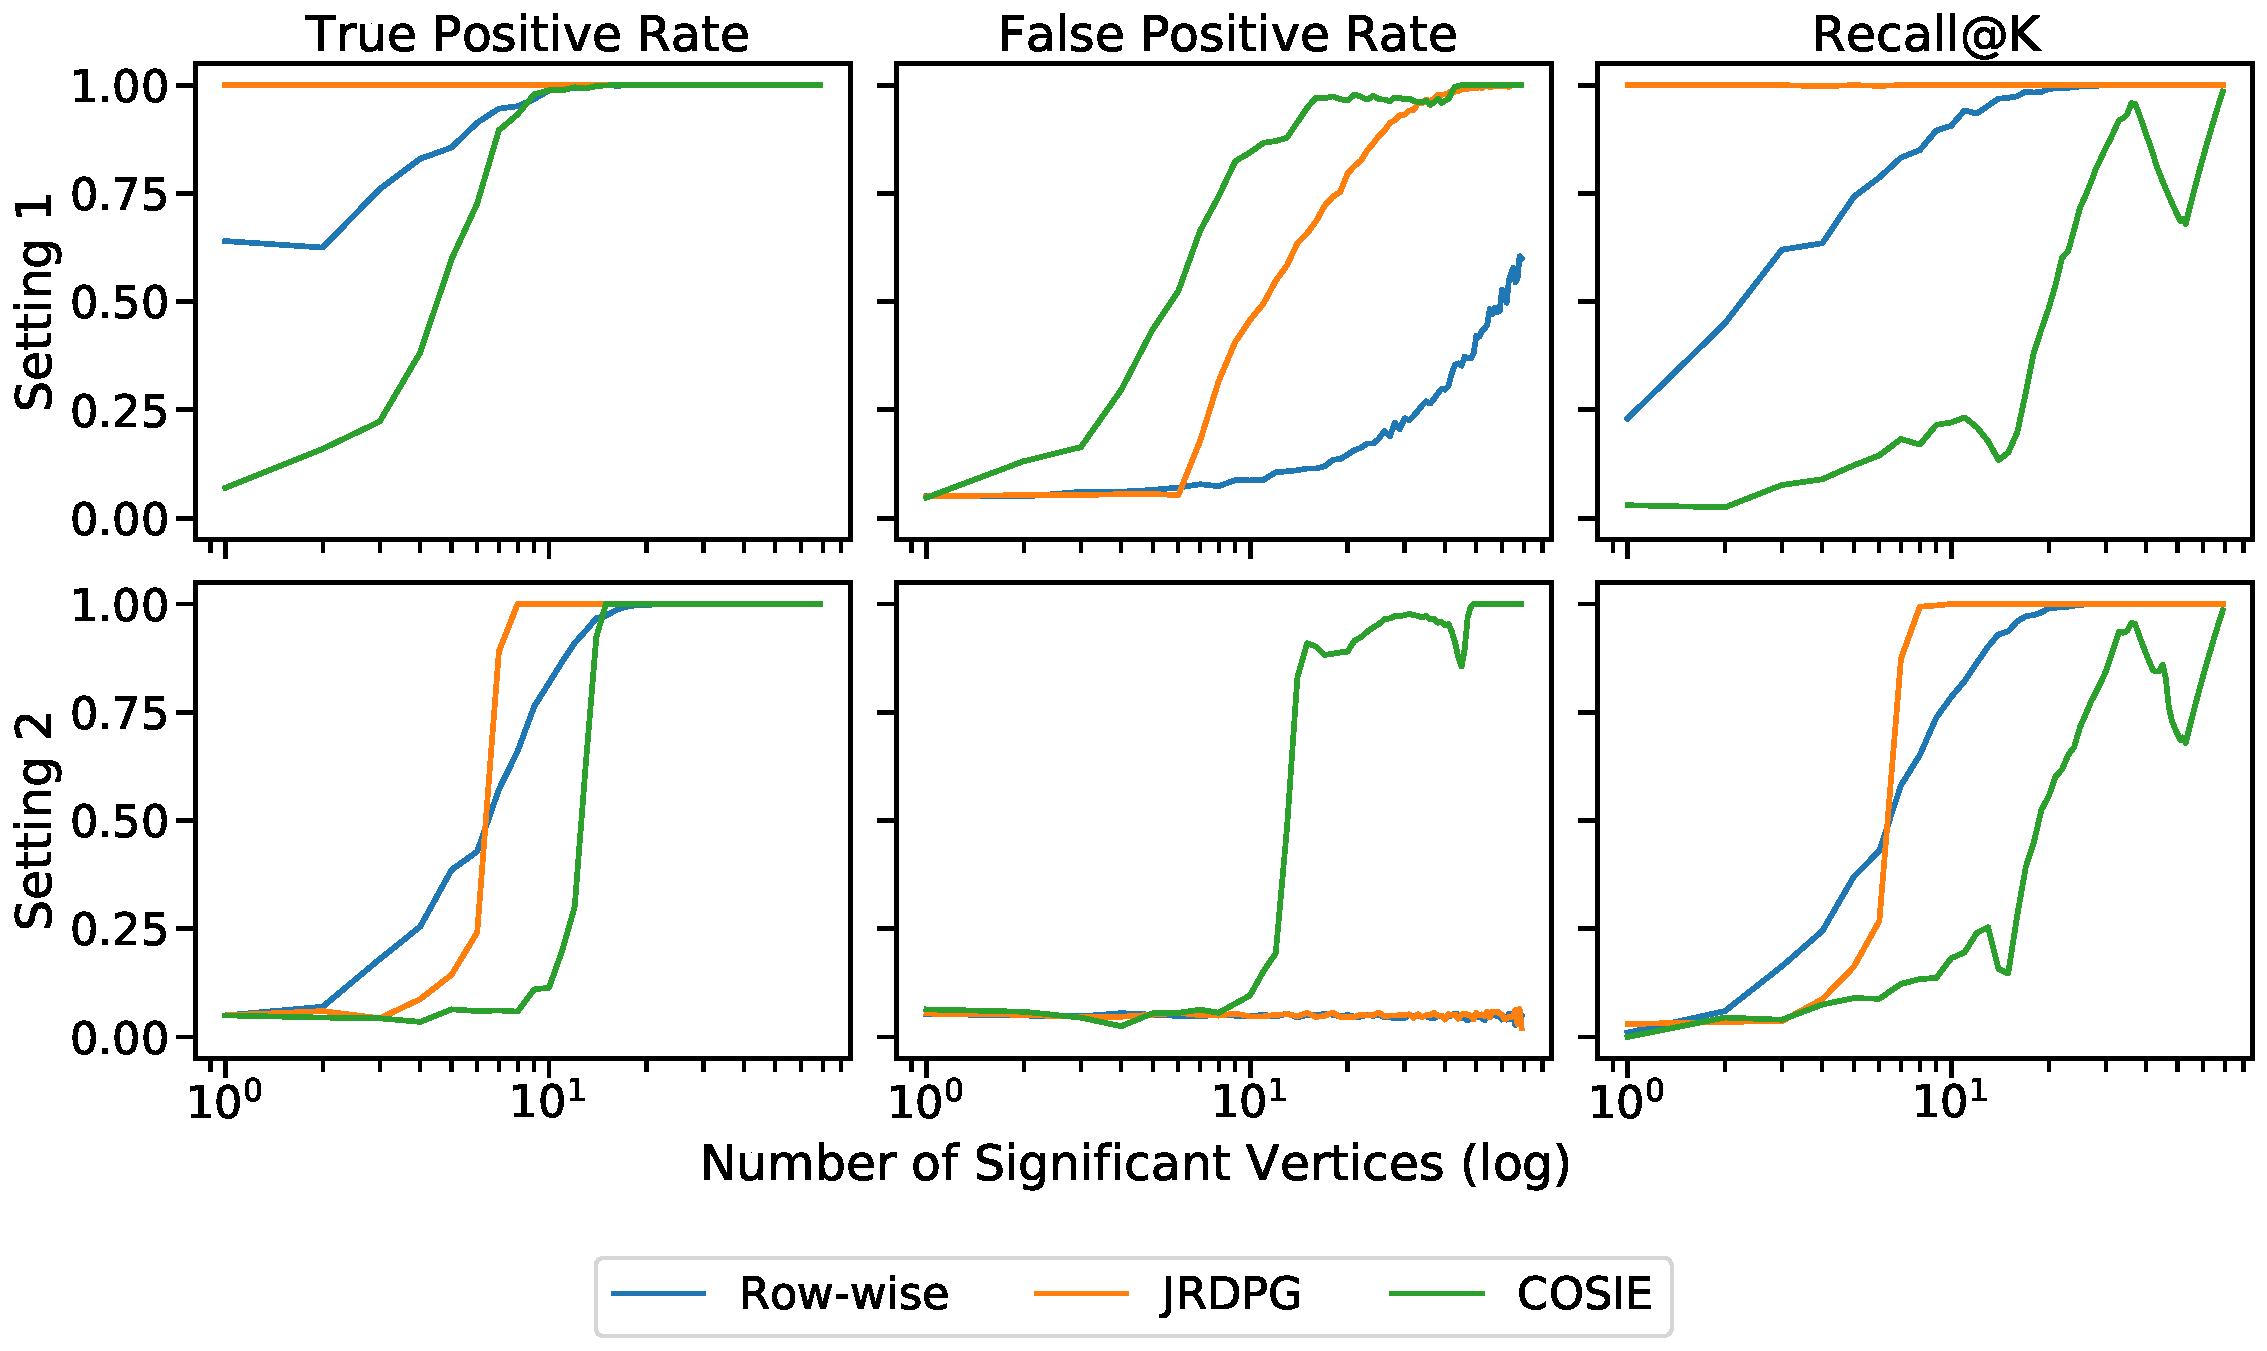
\includegraphics[width=.8\textwidth]{figures/dnd/exp7_new}
    \caption{
    \textbf{Performance for finding significant vertices using various representations of vertices.} We compare a population of graphs from a planted partition stochastic block model ($\sbm$) and another from a symmetric heterogeneous $\sbm$ in two different settings. The number of vertices for each graph is kept constant ($n=70$), but the number of significantly different vertices is varied (x-axis). \textit{(Top row)} In this setting, all three representations are not valid as the false positive rate increases with the number of significant vertices. \textit{(Bottom row)} In this setting, row-wise and joint random dot product graphs ($\jrdpg$) representations are valid while common subspace independent-edge model ($\cosie$) representation is not. 
    In both settings, the sorting of the p-values can be trusted as recall@$K$ increases as number of significant vertices increase.
    }
    \label{fig:exp7}
\end{figure} 


In this section, we test for significant vertices using different representations of vertices. 
Simplest representation is a set of edges, where the corresponding row (or column) of a vertex in the adjacency matrices are collected and tested for difference. 
Another is the low-dimensional latent-space representation using the $\jrdpg$ and $\cosie$ models, and the latent positions of vertices are tested for difference. Since all representations are multivariate, hypothesis are tested using Hotelling's test, which is a multivariate generalization of t-test.

We consider a population of planted partition $\sbm$ and a symmetric heterogeneous $\sbm$ in two different settings. In both settings, the planted partition $\sbm$ has $\B^{(1)} = [0.125, 0.0625; 0.0625, 0.125]$ block probability matrix. In setting 1, the symmetric heterogeneous $\sbm$ has  $\B^{(2)} = [0.125, 0.088; 0.088, 0.25]$ block probability matrix, and in setting 2, $\B^{(2)} = [0.125,  0.0625; 0.0625, 0.25]$. The vertices that belong to the second block, which has the different within-block probability, are considered significant vertices, and we vary the number of vertices that belong to the second block. Total of $m=100$ networks are sampled per population, and the p-values are computed using Hotelling's on each of the three vertex representations for each vertex. Vertices with p-values less than $\alpha=0.05$ after Bonferroni correction are considered significant. The performance is measured via true positive rate (TPR), false positive rate (FPR), and recall@$K$, where $K$ is the number of significant vertices. 

Figure \ref{fig:exp7} shows that the $p$-values cannot necessarily be trusted. That is, in some settings, the significant vertices cannot be trusted due to uncontrolled FPR. However, the sorting of $p$-values can be trusted in both settings. Thus, in situations when the underlying model is not known (i.e. in real data), one should trust the sorting of the $p$-values (or test statistic), but not the magnitudes. 


% \begin{summary}[SUMMARY POINTS]
% Using statistical models, the differences between vertices can be tested. In this test setting, $\jrdpg$ model should be used instead of $\cosie$ model since testing using representations in $\jrdpg$ is both valid and consistent. 
% \end{summary}

\section{Summary}
Here are the summary points:
\begin{enumerate}
    \item Don't rely on network statistics to characterize populations of connectomes. In general, network statistics don't characterize the data that well, and are correlated with one another. Thus, any claim that a specific statistic explains a phenotypic property of a person is based on spurious reasoning.
    \item Do use statistical models developed for networks. Statistical models allow for testing a variety of hypotheses, such as testing for appropriate models and finding significant vertices or communities.
    \item Do use spectral clustering methods for determining community structure. Theoretical and empirical results show that spectral clustering methods can estimate meaningful and trustworthy community structures. However, note that different methods can provide different, but complementary results. 
    \item Do use appropriate hypothesis tests. For example, t-test is appropriate for binary connectomes, but typically invalid and/or under-powered for weighted connectomes.
    \item Don't trust the p-values when performing multiple hypothesis tests. Multiple testing requires corrections to control the false positive rate, all of which are inappropriate for connectomics data.
    \item Do trust the sorting of the p-values when performing multiple hypothesis tests. That is, consider the tests with smallest p-values to reject the null hypothesis as the sorting can be trusted, but not necessarily the magnitudes of p-values. 
\end{enumerate}

Connectomics is an exciting area and is full of interesting ideas, which has led to the emergence of a variety of analysis frameworks. However, the use of statistical modeling in connectomics is still relatively sparse, especially compared to other areas of science. The key conceptual hurdle in statistical modeling of connectomes is to model the entire connectome rather than just edges or features while taking into account the structures and interactions within a connectome. This article provides an overview of current analysis frameworks of connectomics data, and how statistical models can be incorporated to improve current analysis methods. %Below, we summarize the main findings.

\appendix

\addtocontents{toc}{\protect\setcounter{tocdepth}{0}}

\section{Representations}

\subsection{All network features are correlated with one another}\label{sec:bag-of-features-hcp}
The experiment is repeated using the binarized structural connectomes from HCP dataset. For all $1059$ connectomes, which have 70 vertices, the network features are computed. Figure \ref{fig:exp6_hcp} \textit{top row} shows the distributions for all connectomes, and \textit{middle row} and \textit{bottom row} show the distributions after constraining by considering all connectomes with number of edges between $1010$ and $1210$, and then by choosing a network with $1100$ edges at random and choosing all networks with at most $300$ edge differences. Even in real data, constraining the networks produce similar distributions of network statistics. 

\begin{figure}[b!]
    \centering
    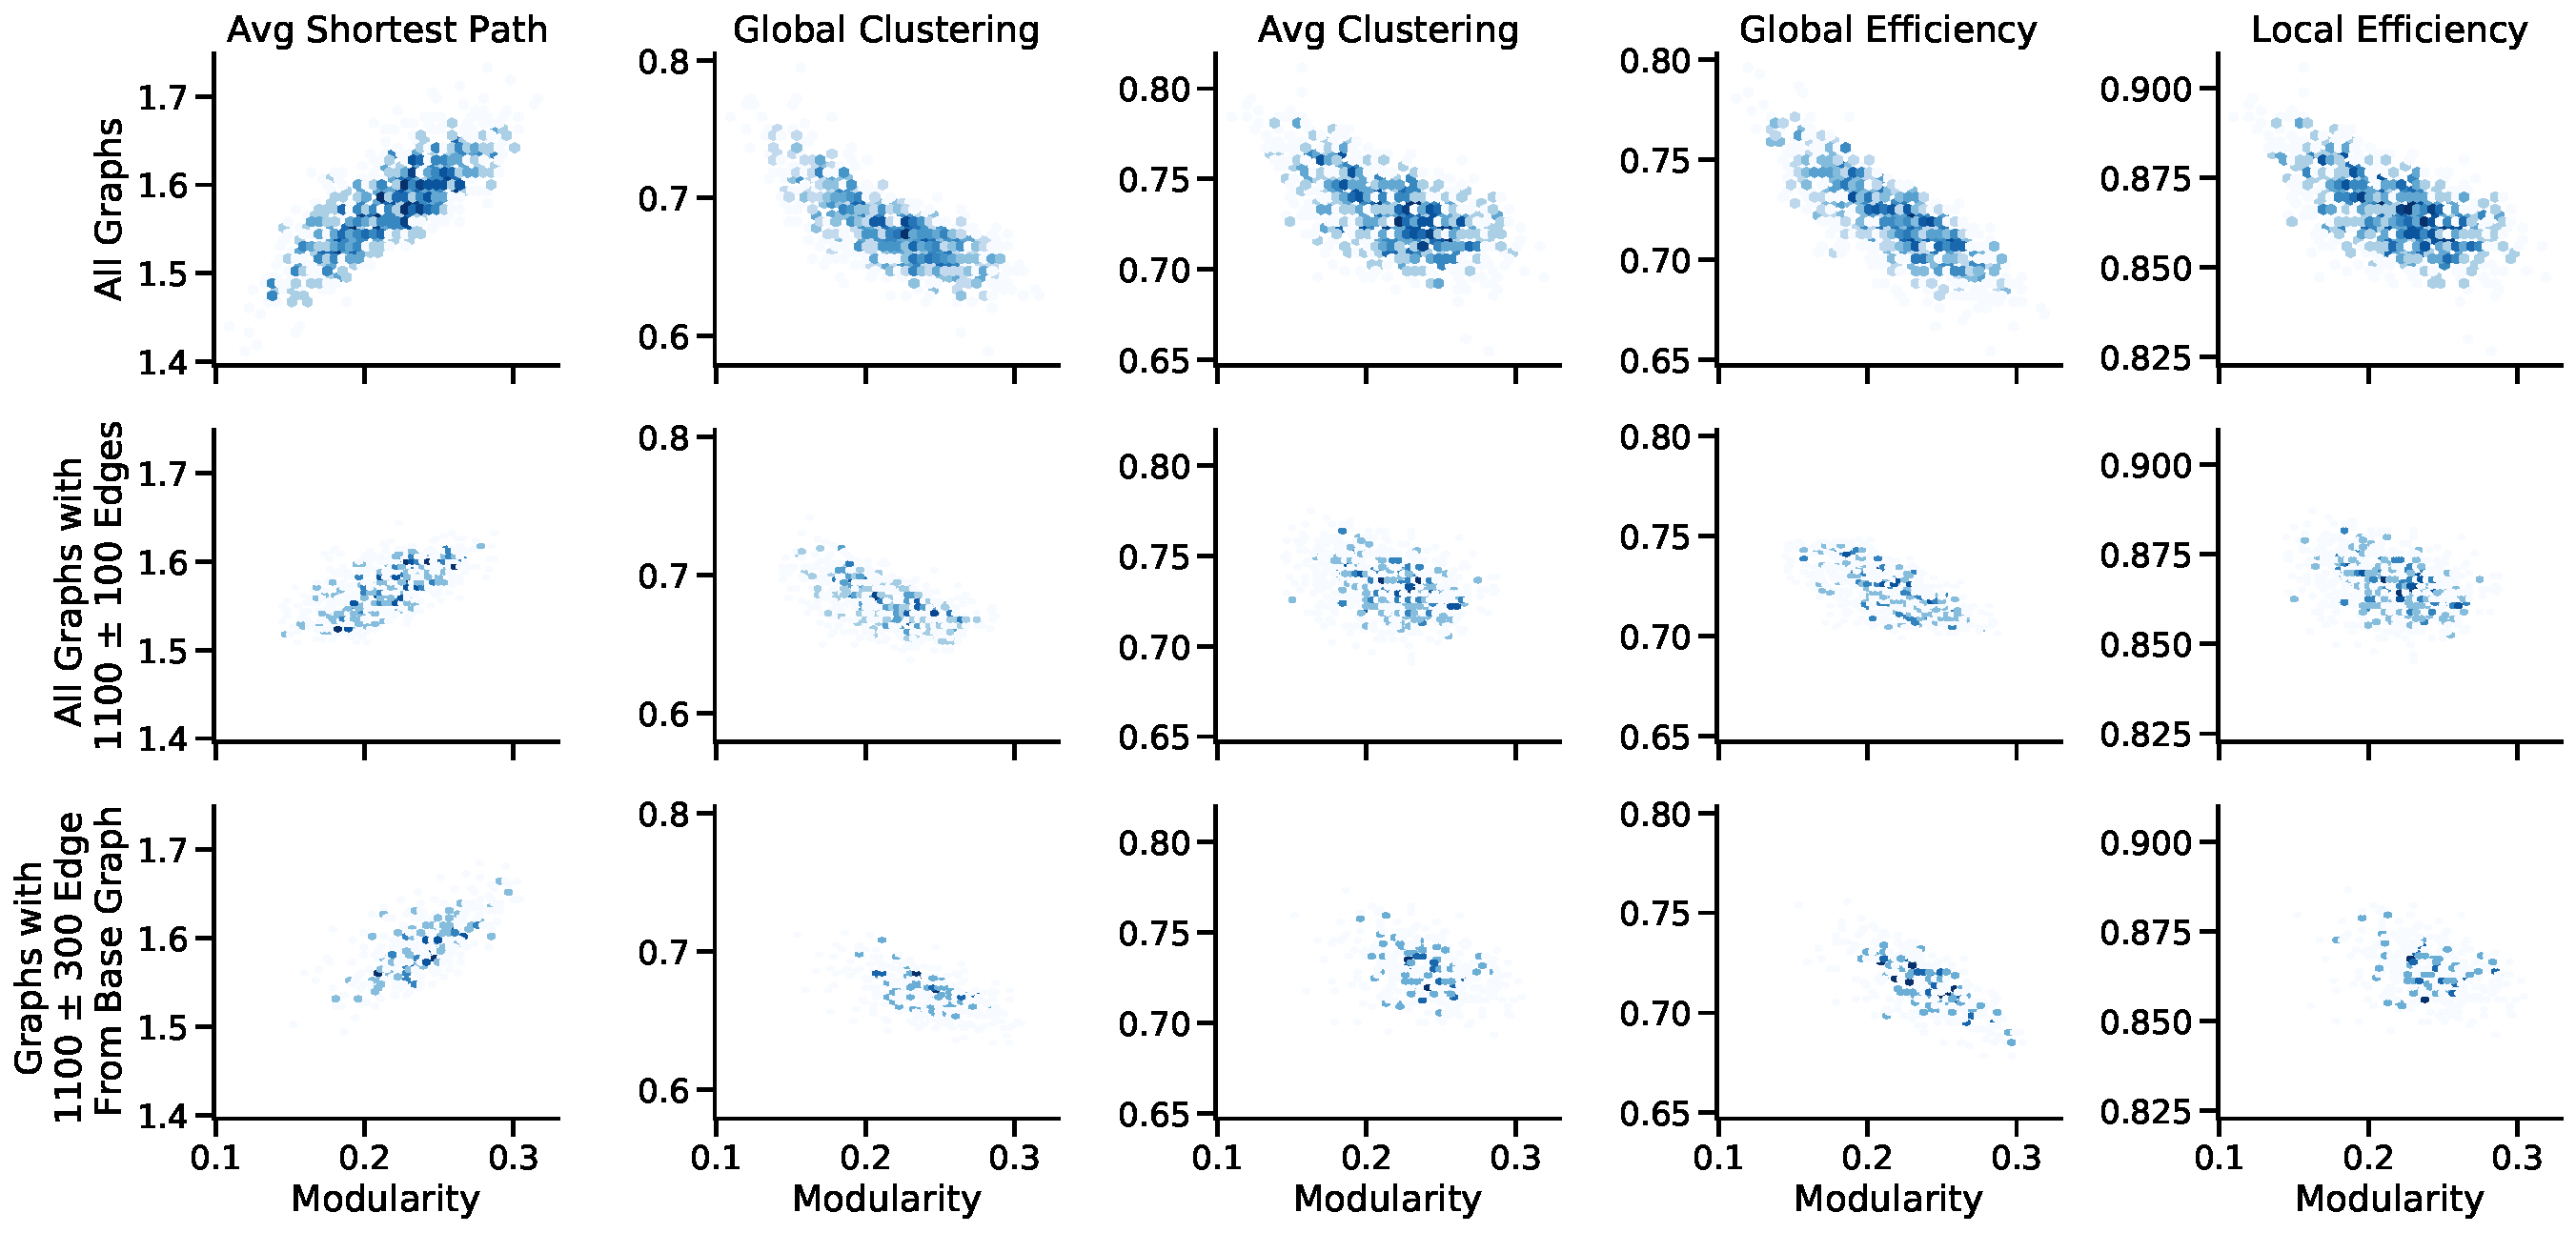
\includegraphics[width=\textwidth]{figures/exp6_hcp.pdf}
    \caption{\textbf{Density plots of network statistics on HCP connectomes.} All connectomes ($N=1059$) have 70 vertices defined by the Deskian parcellation. 
    \textit{(Top row)} The distributions of networks statistics for all HCP connectomes are shown.
    \textit{(Middle Row)} connectomes are constrained by only considering all networks with $1100 \pm 100$ edges.
    and \textit{(Bottom Row)} A base graph with $1100$ edges is chosen at random, and only networks that have differences up to $300$ edges are considered. Similar to the simulated examples, the distributions are qualitatively similar.}
    \label{fig:exp6_hcp}
\end{figure}


\section{Model Extensions}\label{sec:model_extensions}


\subsection{Weighted Models}
% The unweighted graph in Section \ref{sec:unwt_graph} can be extended to the weighted graph model $G = (V, E, w)$, where $V$ and $E$ are the vertices and edges as described previously, and $w : E \rightarrow R$ is a function that assigns a weight to each edge within the graph. Commonly, we are concerned with the case where $R$ is taken to be the non-negative portion of the real line, $[0, \infty)$, and where $E$ is taken to be all possible pairs of vertices $V \times V$. We denote $w_{i,j} \triangleq w(v_i, v_j)$ if $(v_i, v_j) \in E$ for two vertices $v_i, v_j$ which are connected, and $w_{ij} \triangleq 0$ if $v_i, v_j$ are not connected. In this fashion, entries of the adjacency matrix $\A_{ij}$ are taken to be the weights $w_{ij}$ for $i, j \in [n]$. Again, we will take the graphs considered to be undirected; that is, $\A_{ij} = \A_{ji}$ for all $i \neq j$, and with no self-loops; ie, $\textrm{diag}(\A) = \vec 0$. As before, under this specification, the adjacency matrix $\A$ provides a unique representation of $G$.

The single graph models in Section \ref{sec:single_graph_models} can be extended to weighted graphs trivially. For example, in the \textit{a priori} $\sbm$, each distinct community of edges within the graph, simply take the corresponding entries of the adjacency matrix $\A_{ij}$ to take distribution $F_{ij}$ with parameters $\pmb \theta_{ij}$. Adding additional structure to $F_{ij}$ allows the parameters $\theta_{i,j}$ to be estimable for a single graph. In particular, we will be concerned with the Truncated-Normal $\sbm$, where:
\begin{align*}
    \A_{ij}; \vec\tau_i = k, \vec\tau_j = l, \pmb \theta_{kl} \overset{ind}{\sim} \tnorm (\pmb \theta_{kl})
\end{align*}
Where $\pmb \theta_{kl} = (\mu_{k,l}, \sigma^2_{k,l}, \textrm{min}_{k,l}, \textrm{max}_{k,l})$ are the parameters associated with the $k, l$ block of edge weights.

\subsection{Degree-Corrected Models}
In the standard $\sbm$ defined in Section \ref{sec:usbm}, the degree of a vertex, or the expected number of edges incident to a vertex, is constant within each block. Thus, vertices with same block assignment are stochastically equivalent to each other, which can limit practical applications \cite{karrer2011stochastic}. 
In $\mathsf{degree-corrected} \sbm$ ($\dcsbm$),  there is an additional ``promiscuity'' parameter that allows vertices within blocks to have heterogeneous expected degree distributions. 

Similar to the standard $\sbm$, the \textit{a priori} $\dcsbm$ is parameterized by a vertex assignment vector $\vec \tau \in \left\{1, \hdots, K\right\}^n$, a symmetric $K \times K$ block connectivity probability matrix $\B$ with entries in $[0,1]^{K \times K}$, and the degree correction (``promiscuity'') vector $\vec \theta \in\RR^n$. 
The degree correction vector is constrained such that $\sum_i^n \vec \theta_i \mathbb{I} (\tau_i=k)=1$ for $k\in[K]$ where $\mathbb{I}$ is an indicator function. 
The model is $\A\sim\dcsbm_n(\vec\tau, \B, \vec \theta)$ if $\A$ has entries $\A_{ij} \sim \bern(\vec\theta_i \vec\theta_j\B_{kl})$ where $k=\tau_i , l=\tau_j$, for $i, j \in [n]$, and $k, l \in [K]$. 
The \textit{a posteriori} $\dcsbm$ model is additionally parameterized by a block membership probability vector $\vec{\pi} = [\pi_1,\dots,\pi_K]^\top$. The model is $\A \sim \sbm_n(\vec \pi,\B, \vec \theta)$ if $\A$ has entries $\A_{ij} \big | k=\tau_i, l=\tau_j \sim \bern(\vec\theta_i \vec\theta_j\B_{kl})$, where $\tau_i {\sim} \multinomial(\vec \pi)$ for $i \in [n]$. 


% 7. theory
%     1. single graph theory
%         a. "you say i say"
%         b. central limit theorem for ase/lse
%     2. multi graph theory 
%         a. mase/omni
%         c. nonpar + semipar theory
%         d. sgm correlated-SBM/ER theory

\section{Theory for Statistical Models}
In this section, we provide general outlines of the theorems and proofs for statistical models in Section \ref{sec:models} and algorithms in Section \ref{sec:algorithms}.

\subsection{Theory for Single Graph Models}\label{sec:theory_single}

Graph features, such as the ones described in Section~\ref{sec:bag-of-features}, are popularly used to test hypothesis about a graph. However,  the distribution of such features is usually unknown, and even in cases where the asymptotic distribution is available, one needs to proceed with caution as some of the asymptotic results might be misleading \cite{priebe2010you}.  \cite{Rukhin2010} studies the behavior of two simple graph features, namely, the number of edges and the maximum  degree, for testing a simple hypothesis question about the distribution of a graph. While the statistic based on the number of edges achieves a higher power in the limit as the number of vertices grows, a comparative power analysis shows that even for large graphs with $n\leq 10^{24}$, the statistic based on the maximum degree dominates under certain cases.

A body of existing results in statistical inference for spectral embeddings is reviewed more deeply in \cite{athreya2017statistical}. We summarize next some of the main results related to the exposition in this paper. 
In this section, we assume that a sequence of random adjacency  matrices $\{\A_n, n\geq 1\}$ generated from a sequence of latent positions $\{\X_n, n\geq 1\}$, where  $\A_n\sim \rdpg(\X_n)$, $n\geq 1$ is the adjacency matrix of a graph with $n$ vertices, and $\X_n\in\RR^{n\times d}$ are $d$-dimensional latent positions. We write $(\X_n)_i$ to represent the $i$-th row of $\X_n$, and we assume that the rows of $\X_n$, which correspond to the latent positions, are an i.i.d. sample $(\X_1), \ldots, (\X_n)_n\overset{\text{i.i.d.}}{\sim} F$, where $F$ is a distribution with support $\mathcal{X}\subset\RR^d$. We also  assume that the second moment matrix $\mathbf{\Delta} = \mathbb{E}[(\X_n)_1(\X_n)_1^\top]\in\Real^{d\times d}$, has non-zero eigenvalues.   We use $\widehat{\X}_n=\ase(\A_n)\in\Real^{n\times d}$ to denote the $d$-dimensional adjacency spectral embedding of $\A_n$, and $\widetilde{\X}_n = \lse(\A_n)$  to denote its $d$-dimensional Laplacian spectral embedding.


The adjacency spectral embedding ($\ase$) method described in Section~\ref{sec:ase} is a consistent and asymptotically normal estimator for the latent positions of a random dot product graph. In \cite{sussman2012consistent}, it is shown that clustering rows of the $\ase$ of $\A_n$ can consistently recover the communities of an $\sbm$. Consistency of the latent positions for an $\rdpg$ is studied in  \cite{Sussman2014-zq,Lyzinski2014-pe,Lyzinski2017-cq}. In particular, Theorem 5 of  \cite{Lyzinski2017-cq} shows that with probability tending to one, there exists some orthogonal rotation $\W_n\in\Real^{d\times d}$ such that 
\begin{equation*}
    \max_{i\in[n]}\|(\widehat{\X}_n)_i - \W_n(\X_n)_i\| \leq \frac{Cd^{1/2}\log^2 n}{\sqrt{n}}, \label{eq:thm-ASE-const}
\end{equation*}
where $C>0$ is a constant, and hence, the rows of of $\hat{\X}_n$ converge to the rows of $\X_n$, up to some orthogonal rotation, as the number of vertices $n$ grows. 


Distributional results on the rows of the adjacency spectral embedding show that the error in estimating the true latent positions is asymptotically normally distributed. In particular \cite{Athreya2016} showed  a central limit theorem for the rows of the $\ase$ of $\A_n$, in which the latent positions are shown to converge to a mixture of standard multivariate normal distributions, that is, for any $\mathbf{z}\in\RR^{d}$,
\begin{equation}
   \lim_{n\rightarrow\infty} \mathbb{P}\left(\sqrt{n}\left(\widehat{\X}_n\W_n - \X\right)_i\leq \mathbf{z} \right) = \int_{\mathcal{X}}\Phi(\mathbf{z}, \mathbf{\Sigma}(\mathbf{x}))\  dF(\mathbf{x}),\label{eq:thm-ASE-CLT}
\end{equation}
where $\Phi(\mathbf{z}, \mathbf{\Sigma}(\mathbf{x}))$ is the cumulative distribution function of a multivariate normal distribution with mean zero and a covariance matrix $\mathbf{\Sigma}(\mathbf{x})\in\Real^{d\times d}$ that is a function of $\mathbf{x}\in\mathcal{X}$ (see \cite{Athreya2016}, Theorem 1, for an expression of this covariance matrix). 

Similar results to the ones presented above are also available for the Laplacian spectral embedding ($\lse$). In particular, Theorem 3.1 of \cite{tang2018limit} provides an an asymptotic result on the estimation error of the rows of $\widetilde{\X}_n$  with respect to its population version, and Theorem 3.2 shows an analogous result to the one presented in Equation~\eqref{eq:thm-ASE-CLT} to establish the asymptotic normality of the rows of this estimator, that is,
\begin{equation*}
   \lim_{n\rightarrow\infty} \mathbb{P}\left\{\sqrt{n}\left(\W_n(\widetilde{\X}_n)_i - \frac{(\X_n)_i}{\sqrt{\sum_{j}(\X_n)_i^\top (\X_n)_j }} \right)\leq \mathbf{z}\right\}  = \int_{\mathcal{X}}\Phi(\mathbf{z}, \widetilde{\mathbf{\Sigma}}(\mathbf{x}))\  dF(\mathbf{x}),\label{eq:thm-LSE-CLT}
\end{equation*}
for some covariance matrix $\widetilde{\mathbf{\Sigma}}(\mathbf{x})$ which its exact form is presented in \cite{tang2018limit}.

The consistency and asymptotic normality of  $\ase$ and $\lse$ considered in this section  have been recently extended to the $\grdpg$ model  (see Theorems 5-8 in  \cite{rubin2017statistical}). 



\subsection{Theory for Multiple Graph Models}

\subsubsection{Spectral Embeddings}\label{sec:theory_multi}

The results discussed before have been used to develop valid statistical tests for   two-graph hypothesis testing questions. The work of \cite{tang2017semiparametric} studies a semiparametric graph hypothesis testing for the equivalence between the latent positions of the vertices of a pair of graphs. Formally, for each fixed $n$ let $\X_n, \Y_n\in\Real^{n\times d}$ be a sequence of latent positions matrices, and define
$\A_n\sim\rdpg(\X_n)$, $\B_n\sim\rdpg(Y_n)$ as independent random adjacency matrices. The problem of testing the equality of the distributions of $\A_n$ and $\B_n$  is defined as
\begin{equation*}
    \mathcal{H}^n_0:\X_n =_{\W} \Y_n\quad\quad\quad \text{ vs.}\quad\quad\quad \mathcal{H}^n_a:\X_n \neq_{\W} \Y_n,
\end{equation*}
where $\X_n =_{\W}\Y_n$ denotes that $\X_n$ and $\Y_n$ are equivalent up to an orthogonal transformation $\W\in\mathcal{O}_d$, and $\mathcal{O}_d$ is the set of $d\times d$ orthogonal matrices. To define the test statistic, denote  $\widehat{\X}_n = \ase(\A_n)$, $\widehat{\Y}_n=\ase(\B_n)$, and for a matrix $\A\in\Real^{n\times n}$ with singular values $\sigma_1(\A) \geq \ldots\geq \sigma_n(\A)\geq 0$ and largest observed degree $\delta(\A) = \max_{i\in[n]}\sum_{j=1}^n\A_{ij}$, define 
$$\gamma(\A):=\frac{\sigma_d(\A) - \sigma_{d+1}(\A)}{\delta(\A)}.$$ 
Define $T_n$ as the test statistic
\begin{equation*}
    T_n : = \frac{\min_{\W\in\mathcal{O}_d} \|\widehat{\X}_n\W - \widehat{\Y}_n\|_F}{\sqrt{d\gamma^{-1}(\A_n)} + \sqrt{d\gamma^{-1}(\B_n)}}.
\end{equation*}
It is shown in Theorem 3.1 of \cite{tang2017semiparametric} that  $T_n$ is a consistent test for the  hypothesis testing problem described above, in the sense that for any significance level $\alpha$ and $C>1$, then  $\mathbb{P}(T_n> C)\leq \alpha$ for $n$ sufficiently large under $\mathcal{H}^n_0$ (type I error control), and if $\lim_{n\rightarrow\infty}\min_{\W\in\mathcal{O}_d} \|\widehat{\X}_n\W - \widehat{\Y}_n\|_F=\infty$, then $\mathbb{P}(T_n> C)\rightarrow 1$ under $\mathcal{H}^n_a$ (i.e., the type II error vanishes). For specific assumptions and some extensions to other hypothesis testing problems, the reader is referred to \cite{tang2017semiparametric} and \cite{athreya2017statistical}.

When the vertices of the graphs are not necessarily aligned (including cases in which the graphs do not have the same number of vertices), testing equality of latent positions is inappropriate. The work of \cite{tang2017nonparametric} proposes a nonparametric test to determine whether the distribution of the latent positions of the graphs is the same. For a pair of matrices $\X_n\in\Real^{n\times d}$ and $\Y_m\in\real^{m\times d}$ with their rows distributed as $(\X_n)_i\overset{\text{i.i.d.}}{\sim} F$ and $(\Y_m)_i\overset{\text{i.i.d.}}{\sim} G$ and a pair of independent adjacency matrices $\A_n\sim\rdpg(\X_n)$, $\B_n\sim\rdpg(\Y_n)$ , the nonparametric graph hypothesis testing problem is given by
\begin{equation*}
    \mathcal{H}^n_0:F \upVdash G \quad\quad\quad \text{ vs.}\quad\quad\quad \mathcal{H}^n_a: F \nupVdash G,
\end{equation*}
where $F\upVdash G$ indicates equality of the distributions up to an orthogonal transformation. To test such hypothesis, \cite{tang2017nonparametric} proposes to use the following test statistic
\begin{align*}
    U_{n,m}(\X, \Y)=& \frac{1}{n(n-1)}\sum_{j\neq i}\kappa(X_i, X_j)-\frac{2}{mn}\sum_{i=1}^n\sum_{k=1}^m\kappa(X_i, Y_k)\\
    & + \frac{1}{m(m-1)}\sum_{l\neq k}\kappa(Y_k, Y_l),
\end{align*}
where $\kappa:\mathcal{X}\times \mathcal{X}\rightarrow\Real$ is a positive definite kernel. In \cite{tang2017nonparametric}, Theorem 1, it is shown that $U_{n,m}(\X, \Y)$ is a consistent and unbiased estimate of the maximum mean discrepancy \cite{gretton2012kernel} between the distributions $F$ and $G$. Furthermore, under the null hypothesis, the quantity $(m+n)U_{n,m}(\X, \Y)$ converges in distribution to an infinite weighted sum of independent chi-squared random variables as $n,m\rightarrow \infty$, provided that $\frac{n}{n+m}\rightarrow \rho \in (0, 1)$.  Moreover, when the latent positions are used in place of the true latent positions, then Theorem 4 of \cite{tang2017nonparametric} shows that the difference between $U_{n,m}(\widehat{\X}, \widehat{\Y})$  and $U_{n,m}(\X, Y)$ converges to zero sufficiently fast to yield a consistent test procedure.

% Under the null hypothesis that $F = G$ (up to some orthogonal transformations), 
% \begin{equation*}
%     (m+n)(U_{n,m}(\widehat{\X}, \widehat{\Y}) - U_{n,m}({\X}, {\Y}\W_{n,m})) \overset{a.s.}{\rightarrow} 0.
% \end{equation*}
% Under the alternative hypothesis, 
% \begin{equation*}
%     \frac{(m+n)}{\log^2(m+n)}(U_{n,m}(\widehat{\X}, \widehat{\Y}) - U_{n,m}({\X}, {\Y}\W_{n,m})) \overset{a.s.}{\rightarrow} 0
% \end{equation*}

% Suppose that $n,m\rightarrow\infty$ and $\frac{m}{m+n}\rightarrow\rho\in(0,1)$.

%Theorem 43 of \cite{athreya2017statistical} (consistency of nonpar)

The work of \cite{levin2017central} studies the omnibus embedding described in Section~\ref{sec:omni} under the joint random dot product graph ($\jrdpg$) model, where $(\A^{(1)}, \ldots, \A^{(m)})\sim\jrdpg(\X_n)$, and the rows of $\X_n\in\Real^{n\times d}$ are an i.i.d. sample from some distribution $F$. Let $\widehat{\mathbf{O}}\in\Real^{mn\times mn}$ be the omnibus embedding of $\A^{(1)}, \ldots, \A^{(m)}$ and $\widehat{\Z} = \ase(\mathbf{O})\in\Real^{mn\times d}$.
Under this setting, it is shown in Lemma 1 of \cite{levin2017central} that the rows of $\widehat{\Z}_n$ are a consistent estimator of the latent positions of each individual graph  as $n\rightarrow\infty$, and that
\begin{equation}
\max_{i\in[n],j\in[m]}\|(\widehat{\Z}_n)_{(j-1)n + i} - \W_n(\X_n)_{i}\| \leq \frac{C\sqrt{m}\log(mn)}{\sqrt{n}}. \label{eq:OMNI-consistency}    
\end{equation}
Furthermore, a central limit theorem for the rows of the omnibus embedding  asserts that
\begin{equation}
   \lim_{n\rightarrow\infty} \mathbb{P}\left\{\sqrt{n}\left(\W_n(\widehat{\Z}_n)_{(j-1)n + i} - (\X_n)_i\right)\leq \mathbf{z}\right\}  = \int_{\mathcal{X}}\Phi(\mathbf{z}, \widehat{\mathbf{\Sigma}}(\mathbf{x}))\  dF(\mathbf{x}),\label{eq:thm-OMNI-CLT}
\end{equation}
for some covariance matrix $\widehat{\Sigma}(\mathbf{x})$ (see Theorem 1 of \cite{levin2017central} for an exact expression). In recent work, \cite{draves2020bias} extended the study of the omnibus embedding and provided results analogous to the ones in Equations~\eqref{eq:OMNI-consistency} and \eqref{eq:thm-OMNI-CLT} under a more general model that allows for differences in the latent positions of each graph.


The $\cosie$ model described in Section~\ref{sec:cosie} describes multiple networks with expected probability matrices that share the same common invariant subspace. It is shown in \cite{arroyo2019inference} that the $\mase$ algorithm (see Section~\ref{sec:mase}) is a consistent estimator for this common invariant subspace, and produces asymptotically normally distributed estimates for the individual symmetric matrices. Specifically, let $\V_n\in\Real^{n\times d}$ be
a sequence of orthonormal matrices and $\R^{(1)}_n, \ldots, \R^{(m)}_n\in\Real^{d\times d}$ a sequence of score matrices such that $\mathbf{P}^{(l)}_n=\V_n\R^{(l)}_n\V_n^\top\in[0,1]^{n\times n} $, $(\A_n^{(1)}, \ldots, \A_n^{(m)})\sim \cosie(\V_n;, \R^{(1)}_n, \ldots, \R^{(m)}_n)$, and $\widehat{\V}, \widehat{\R}^{(1)}_n, \ldots, \widehat{\R}^{(1)}_n$ be the estimators obtained by $\mase$. Under appropriate regularity conditions (see Theorem 3 of \cite{arroyo2019inference}), the estimate for $\V$ is consistent as $n,m\rightarrow\infty$, and there exists some constant $C>0$ such that
        \begin{equation*}
			\mathbb{E}\left[\min_{\W\in\mathcal{O}_d}\|\widehat{\V}-\V\W\|_F\right] \leq C\left(\sqrt{\frac{1}{mn}} + {\frac{1}{n}}\right). \label{eq:theorem-bound}
		\end{equation*}
    In addition, the entries of $\widehat{\mathbf{R}}^{(l)}_n$, $l\in[m]$ are asymptotically normally distributed. Namely, there exists a sequence of orthogonal matrices $\W$ such that
		$$\frac{1}{\sigma_{l,j,k}}\left(\widehat{\R}^{(l)}_n - \W^\top\R^{(l)}_n\W + \Hmat_m^{(l)}\right)_{jk} \overset{d}{\rightarrow} \mathcal{N}(0, 1), $$
		as $n\rightarrow\infty$, where
		$\mathbb{E}[\|\Hmat_m^{(l)}\|]=O\left(\frac{d}{\sqrt{m}}\right)$ and $\sigma^2_{l,j,k} = O(1)$. 
		For a  precise statement about the joint distribution of the entries of $\widehat{\mathbf{R}}_n^{(i)}$, see Theorem 7 in \cite{arroyo2019inference}.


\subsubsection{Graph Matching for Correlated Networks } Given a pair of graphs $\A_n$ and $\B_n$ with $n$ vertices each, the graph matching problem tries to find a correspondence between their vertices. A body of literature has studied the feasibility of finding the correct matching under different random graph models, including correlated  Erd\H{o}s-R\'enyi  \cite{Lyzinski2013-fq,cullina2016improved} and Bernoulli graphs
\cite{lyzinski2015graph}. In this section we review some of the results for the correlated Erd\H{o}s-R\'enyi model described in Section~\ref{sec:correlated-graphs}.

Formally, given parameters $\rho_n\in[0,1]$ and $q_n \in(0, 1-\xi_1)$ for some small $\xi_1>0$, the $n\times n$ adjacency matrices $\A_n$ and $\B_n$ are distributed as correlated Erd\H{o}s-R\'enyi if their marginal distributions are $\A_n\sim\er_n(q_n)$, $\B_n\sim\er_n(q_n)$, but the edge pairs satisfy $\text{Corr}((\A_n)_{ij},(\mathbf{Q}_n^\top\B_n\mathbf{Q}_n)_{ij})=\rho_n$, where $\mathbf{Q}_n\in\mathcal{P}_n$ is a permutation matrix that gives the correct alignment between the vertices (here $\mathcal{P}_n$ denotes the set of $n\times n$ permutation matrices). The work of \cite{Lyzinski2013-fq}  studies the feasibility of finding $\mathbf{Q}_n$ by solving the optimization problem defined in Equation~\eqref{eq:GMP}. In particular, it is shown that there exists positive constants $c_1, c_2$ such that if $\rho_n\geq c_1\sqrt{\frac{\log n}{n}}$ and $q_n\geq c_2 \frac{\log n }{n}$, then $\mathbf{Q}_n$ can be correctly recovered  with probability 1 for $n$ sufficiently large (Theorem 1 of \cite{Lyzinski2013-fq}). 

While the solution of the quadratic assignment problem \eqref{eq:GMP} can correctly recover the vertex alignment in theory, it is computationally challenging to solve the optimization problem. In the presence of $s_n$ seed vertices with known correspondence between the graphs, \cite{Lyzinski2013-fq} introduced an efficient polynomial algorithm to recover the alignment of the remaining $n-s_n$ vertices.
Theorem 2 of \cite{Lyzinski2013-fq} shows that this method can correctly recover $\mathbf{Q}_n$ in the setting where $\xi_2 < p_n<1-\xi_2<1$ and $\xi_2 < \rho_n < \xi_2$ for some $\xi_2>0$ in the presence of a logarithmic number of seeds (i.e. $s_n\geq c_3 \log n$ for some $c_3>0$).

\section{Data Descriptions}
The following two datasets are analyzed using the algorithms and models described Sections \ref{sec:models} and \ref{sec:algorithms}. Section \ref{sec:single_app} primarily focuses on the \textit{Drosphila} connectome, while Section \ref{sec:multi_app} primarily focuses on HCP connectomes.

\subsection{\textit{Drosphila} Larval Mushroom Body Data Description}\label{sec:drosphila}
The connectome was estimated from serial-section electron microscopy (EM) of an L1 \textit{Drosophila} larva \cite{eichler2017complete}. For the mushroom body (MB) subcircuit, the graph was defined by manually identifying synapses in the EM volume, and tracing the pre- and post-synaptic partners through the EM volume back to their cell bodies. Each node in this graph represents an individual neuron, and each edge consists of one or more synapses between those neurons. Thus, edge weights are the number of synapses between neurons. 

Each node in the graph also has an associated cell type: Kenyon cell (KC), projection neuron (PN), MB input neuron (MBIN), and MB output neuron (MBON). Additionally, we can categorize neurons based on hemisphere (which side of the brain each neuron was on), and neuron pair (for most neurons, a homologous pair neuron in the other hemisphere was identified by morphological comparison).

\subsection{HCP Data Description}\label{sec:hcp}
We used publicly available diffusion MRI (dMRI) and structural MRI (sMRI) data from the S1200 (2017) release of the Human Connectome Project (HCP) Young Adult study, acquired by the Washington University in St. Louis (WUSTL) and the University of Minnesota (Minn) \cite{hcp1, hcp2}. Out of the 1206 participants released, 1059 had viable dMRI for processing. 

Connectomes were estimated using the ndmg pipeline \cite{Kiar188706}. Briefly, the dMRI scans were pre-processed for eddy currents using FSL's \texttt{eddy-correct} \cite{fsl1}. FSL's ``standard" linear registration pipeline was used to register the sMRI and dMRI images to the MNI152 atlas \cite{fsl1,fsl2,fsl3,mni152}.A tensor model is fit using DiPy \cite{dipy} to obtain an estimated tensor at each voxel. A deterministic tractography algorithm is applied using DiPy's EuDX \cite{dipy,eudx} to obtain streamlines, which indicate the voxels connected by an axonal fiber tract. We used a modified version of Desikan–Killiany–Tourville (DKT) parcellation \cite{DKT}  to define the ROIs. Graphs are formed by counting the number of fibers between a pair of ROIs. 

% TODONE seems like drosophila is only in 6, and HCP is only in 7? if so, you can absorb this section into the appropriate subsections. 
% TODO@jv - not quite true since the graph matching is in multi-graphs

\section{Single Graph Applications}\label{sec:single_app_appendix}

\subsection{Independent Edge Modelling}\label{sec:siem_wt}
In Figure \ref{fig:dros_siem}, we investigate the appropriateness of different $\siem$ for the weighted \textit{Drosophila} connectome, similar to Figure \ref{fig:siem_uwt}.  Our goal is the same as previously; ie, to identify whether within-hemisphere connectivity exceeds between-hemisphere connectivity. Figure \ref{fig:dros_siem}(A) shows a comparison of the within and the between-hemisphere edge blocks. The within-hemisphere edge blocks appear to have a higher proportion of non-zero edges than the between-hemisphere edge blocks. This effect is significant, with the interpretation that within-hemisphere connectivity exceeds between-hemisphere connectivity at $\alpha=.05$ (Mann-Whitney Wilcoxon Test, $n=103041$, $p$-value$=0.0$). Figure \ref{fig:dros_siem}(B) shows a comparison of the homotopic and heterotopic edge blocks. The homotopic edges appear to have a higher proportion of non-zero edges with smaller edge weights, and a similar proportion of non-zero edges with larger edge weights. Homotopic connectivity significantly exceeds heterotopic connectivity at $\alpha=.05$ (Mann-Whitney Wilcoxon Test,  $n=103041$, $p$-value$=0.0$).

\begin{figure}
    \centering
    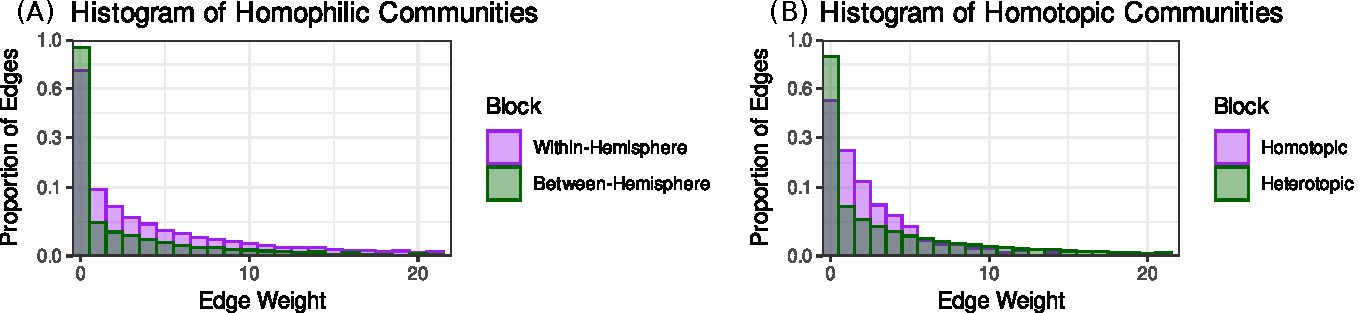
\includegraphics[width=\linewidth]{figures/dros_siem.pdf}
    \caption{\textbf{Goodness of fit of homophilic and homotopic $\siem$ for weighted \textit{Drosophila} mushroom body}. \textbf{(A)} A comparison of the homophilic communities as determined by the hemispheres of incident vertices. The relative heights of the bars are normalized by the square root of the proportion due to the fact that the substantial majority of edges in both communities have a weight of $0$. Within-hemisphere edges appear to have greater connectivity than between-hemisphere edges. Within-hemisphere edges show significantly higher connectivity than between-hemisphere edges (Mann-Whitney Wilcoxon Test, $n=103041$, $p$-value$=0.0$). \textbf{(B)} A comparison of the homotopic edge communities, where homotopic edges are those that are incident a bilateral pair of vertices. Homotopic edges appear to have greater connectivity than heterotopic edges. Homotopic connectivity significantly exceeds heterotopic connectivity (Mann-Whitney Wilcoxon Test, $n=103041$, $p$-value$=0.0$).}
    \label{fig:dros_siem}
\end{figure}

In Figure \ref{fig:siem_os_mri} we explore the appropriateness of the $\siem$ for diffusion connectomes from the HCP Dataset. Figure \ref{fig:siem_os_mri}(A) shows the average diffusion connectome over all participants in the study. Figure \ref{fig:siem_os_mri}(B) shows the distribution of edge-weights within-hemisphere versus between-hemisphere. The diffusion connectomes appear to possess homophily; ie, high within-hemisphere connectivity, with lower between-hemisphere connectivity. To test this observation, we employ the $\texttt{MWW}$ test. All $1059$ diffusion connectomes have significantly higher within-hemisphere connectivity than between-hemisphere connectivity at $\alpha=.05$ after Bonferroni correction \cite{Bonferroni1936-ip}.

\begin{figure}
    \centering
    \includegraphics[width=\linewidth]{figures/hcp_siem.pdf}
    \caption{\textbf{Goodness of fit of homophilic $\siem$ for diffusion connectomes}. \textbf{(A)} The average diffusion connectome over $N=1059$ connectomes with $n=70$ vertices from the HCP dataset shows that diffusion connectomes appear to be homophilic, with higher within-hemisphere connectivity than between-hemisphere connectivity. Hemisphere annotations are provided for regions in the left and right hemispheres. Within-hemisphere edges are edges whose vertices are both located in the same hemisphere of the brain (the on-diagonal blocks). \textbf{(B)} Density estimates for the within-hemisphere and between-hemisphere edges for each of the $N=1059$ connectomes. Homophily is tested per-graph using the Mann-Whitney Wilcoxon Test to detect whether the on-diagonal blocks have higher connectivity than the off-diagonal blocks. All $N=1059$ diffusion connectomes have significantly higher within-hemisphere connectivity than between-hemisphere connectivity after Bonferroni correction at $\alpha=.05$, and the maximum corrected $p$-value is on the order of $10^{-21}$.}
    \label{fig:siem_os_mri}
\end{figure}

\subsection{Identification of Optimal Block Structure}\label{sec:sbm_est_wt}

In Figure \ref{fig:dros_sbm_est}, we investigate the appropriate block structure for the weighted \textit{Drosophila} mushroom body. \ref{fig:dros_sbm_est}(I) shows the distribution of edges associated with each block of $\B$, where the $n=319$ vertices in either the left or right hemisphere are partitioned according to hemisphere. Again, the weighted \textit{Drosophila} mushroom body is directed, so assuming symmetry would not be sensible. We investigate whether the \textit{Drosophila} mushroom body is $\er$, planted partition, symmetric heterogeneous, or asymmetric heterogeneous $\sbm$, using Kruskal-Wallis (KW), Distance Correlation (DCorr), and Analysis of Variance (ANOVA). Each method identifies the planted partition $\sbm$ as the most appropriate block model. This has the interpretation that the best-fit $\sbm$ includes a shared distribution for the on-diagonal (Left,Left) and (Right,Right) blocks, and a different shared distribution for the off-diagonal (Left,Right) and (Right,Left) blocks. An important considerations is that while the best-fit $\sbm$ is symmetric, the graph itself is directed. This has the implication that while the best-fit $\sbm$ would posit that edges in the (Left,Right) and (Right,Left) blocks have the same distribution, realizations of the (Left,Right) and (Right,Left) block will not necessarily be identical.

\begin{figure}
    \centering
    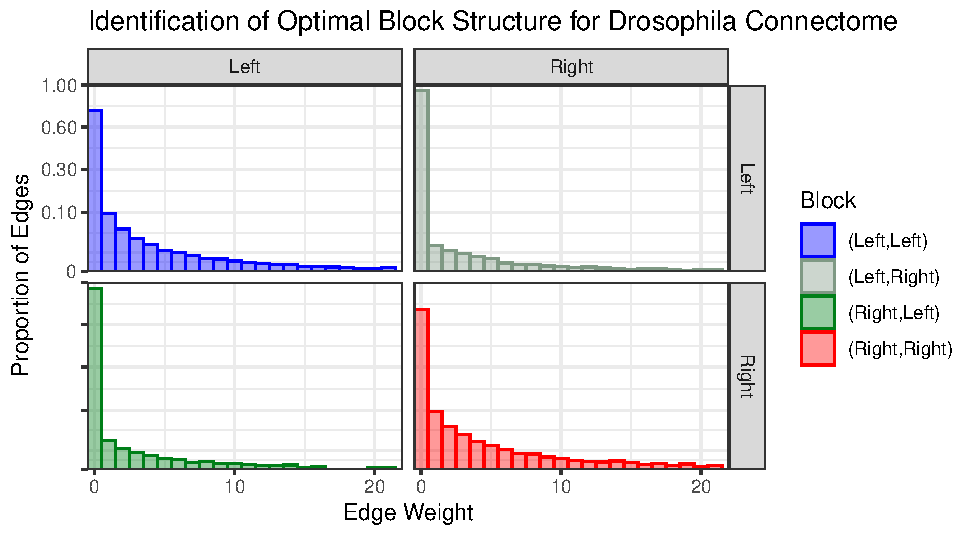
\includegraphics[width=.8\linewidth]{figures/dros_sbm_est.pdf}
    \caption{\textbf{Identifying the appropriate block structure of the \textit{Drosophila} mushroom body}. We investigate the appropriate block structure in the \textit{Drosophila}  mushroom body, with $n=319$ vertices in the left or right hemisphere. Each block corresponds to the proportion of edges with the listed edge weight. As in Figure \ref{fig:dros_siem}, the proportion of edges are shown on a scale in which bar height corresponds to the square root of the proportion, due to the presence of a large number of zero-weight edges. We investigate whether the $\sbm$ is $\er$, planted partition, symmetric heterogeneous, or asymmetric heterogeneous $\sbm$, using Kruskal-Wallis (KW), Distance Correlation (DCorr), and Analysis of Variance (ANOVA) for model selection. All approaches identify planted partition $\sbm$ as the best-fit block structure.}
    \label{fig:dros_sbm_est}
\end{figure}

In Figure \ref{fig:nested_sbm_ts_mri}, we investigate the appropriate block structure for diffusion connectomes, analogous to the single graph investigations using the \textit{Drosophila} mushroom body in Figure \ref{fig:dros_sbm_est}. Panel \textbf{(A)} demonstrates the distribution of edges associated with each block of $\B$. Panel \textbf{(B)} shows the fraction of diffusion connectomes that accept each of the candidate hypotheses, using $3$ different approaches for weighted graph model selection: Kruskal-Wallace  \cite{Kruskal1952-kj}, Distance Correlation (Dcorr) \cite{Szekely2007-mm}, and Ananysis of Variance (ANOVA) \cite{Fisher1925-xm,Scheffe1999-pi}. Diffusion connectomes tend to display planted partition structure across all model selection approaches.

\begin{figure}
    \centering
    \includegraphics[width=\linewidth]{figures/hcp_block_est.pdf}
    \caption{\textbf{Identification of appropriate block structure in diffusion connectomes}. We investigate the appropriate block structure in the diffusion connectomes from the HCP Dataset, with $n=70$ vertices, and $N=1059$ graphs. \textbf{(A)} the empirical distribution of edges for each of the $4$ blocks of edges for each between and within-hemisphere pair for the left and right hemispheres respectively. As the diffision connectomes are inherently symmetric, the off-diagonal blocks are inherently symmetric. The hypothesized models are that the graph is $\er$, planted partition $\sbm$ (Plant Part.), or the symmetric heterogeneous $\sbm$ (Sym. Het.). \textbf{(B)} The number of connectomes from the dataset for which the specified candidate model is selected. All methods for selection of optimal block structure identify diffusion connectomes as planted partition $\sbm$, which has the interpretation that the optimal structure is to assume that the on-diagonal left and right blocks share a common distribution that differs from the off-diagonal contralateral blocks. This conclusion holds across all diffusion connectomes within the dataset.}
    \label{fig:nested_sbm_ts_mri}
\end{figure}



\section{Multiple Graph Applications}\label{sec:multi_app_appendix}

\subsection{Testing for Significant Edges in Weighted Networks} \label{sec:exp2}
We consider two populations of networks generated from a 2 block $\sbm$, except edges are now sampled from truncated normal distribution to emulate correlation matrices. All networks have $n=20$ vertices and $\vec{\pi} = \bracks*{0.25, 0.75}$. The block edge distribution matrices for each population is given by
\begin{align*}
    \B^{(1)} &= 
    \begin{bmatrix}
        \tnorm(0, 0.25, -1, 1)   & \tnorm(0, 0.25, -1, 1) \\
        \tnorm(0, 0.25, -1, 1)   & \tnorm(0, 0.25, -1, 1) 
    \end{bmatrix} \\
    \B^{(2)} &= 
    \begin{bmatrix}
        \tnorm(0 + \delta, 0.25 + \phi, -1, 1)   & \tnorm(0, 0.25, -1, 1) \\
        \tnorm(0, 0.25, -1, 1)   & \tnorm(0, 0.25, -1, 1) 
    \end{bmatrix}
\end{align*}
where $\tnorm(\mu, \sigma^2, a, b)$ denotes a truncated normal distribution with mean $\mu$ and variance $\sigma^2$ such that all values are in $[a, b]$. Total of $m$ networks are sampled ($m/2$ networks per population). One population has the same edge weight distribution for all edges, and the second population's first block edges has either a different mean, $\delta$, or variance, $0.25 + \phi$.
For each edge, test statistics are computed with three different tests: 1) t-test, 2) Mann-Whitney (MW) U test, which is a non-parametric test of medians, and 3) two-sample Kolomogrov-Smirnov (KS) test, which is test of two distributions. Similar to experiment 1, the test statistics are sorted to find the ten most significant edges, and the performance is evaluated with recall.

Figure \ref{fig:exp2} shows the results by varying the sample size, mean, and variance. Figure \ref{fig:exp2} top row shows that all three tests can identify edges that are different in means, and that no particular test is superior than another. 
%Even at low sample sizes ($m=100$), all three tests can perfectly identify significant edges At effect size as low as $\delta = 0.3$ with sample size $m=1000$.
Figure \ref{fig:exp2} bottom row shows that only KS test can detect changes in variance when the means are kept the same. This is because t-test and MW test ultimately test for differences in centrality (e.g. mean or median), where as KS tests for any differences between a pair of observed distributions. 
% but large samples size ($m=1000$) and large effect size ($\phi\geq 2.5$) are required for high recall. 

\begin{figure}
    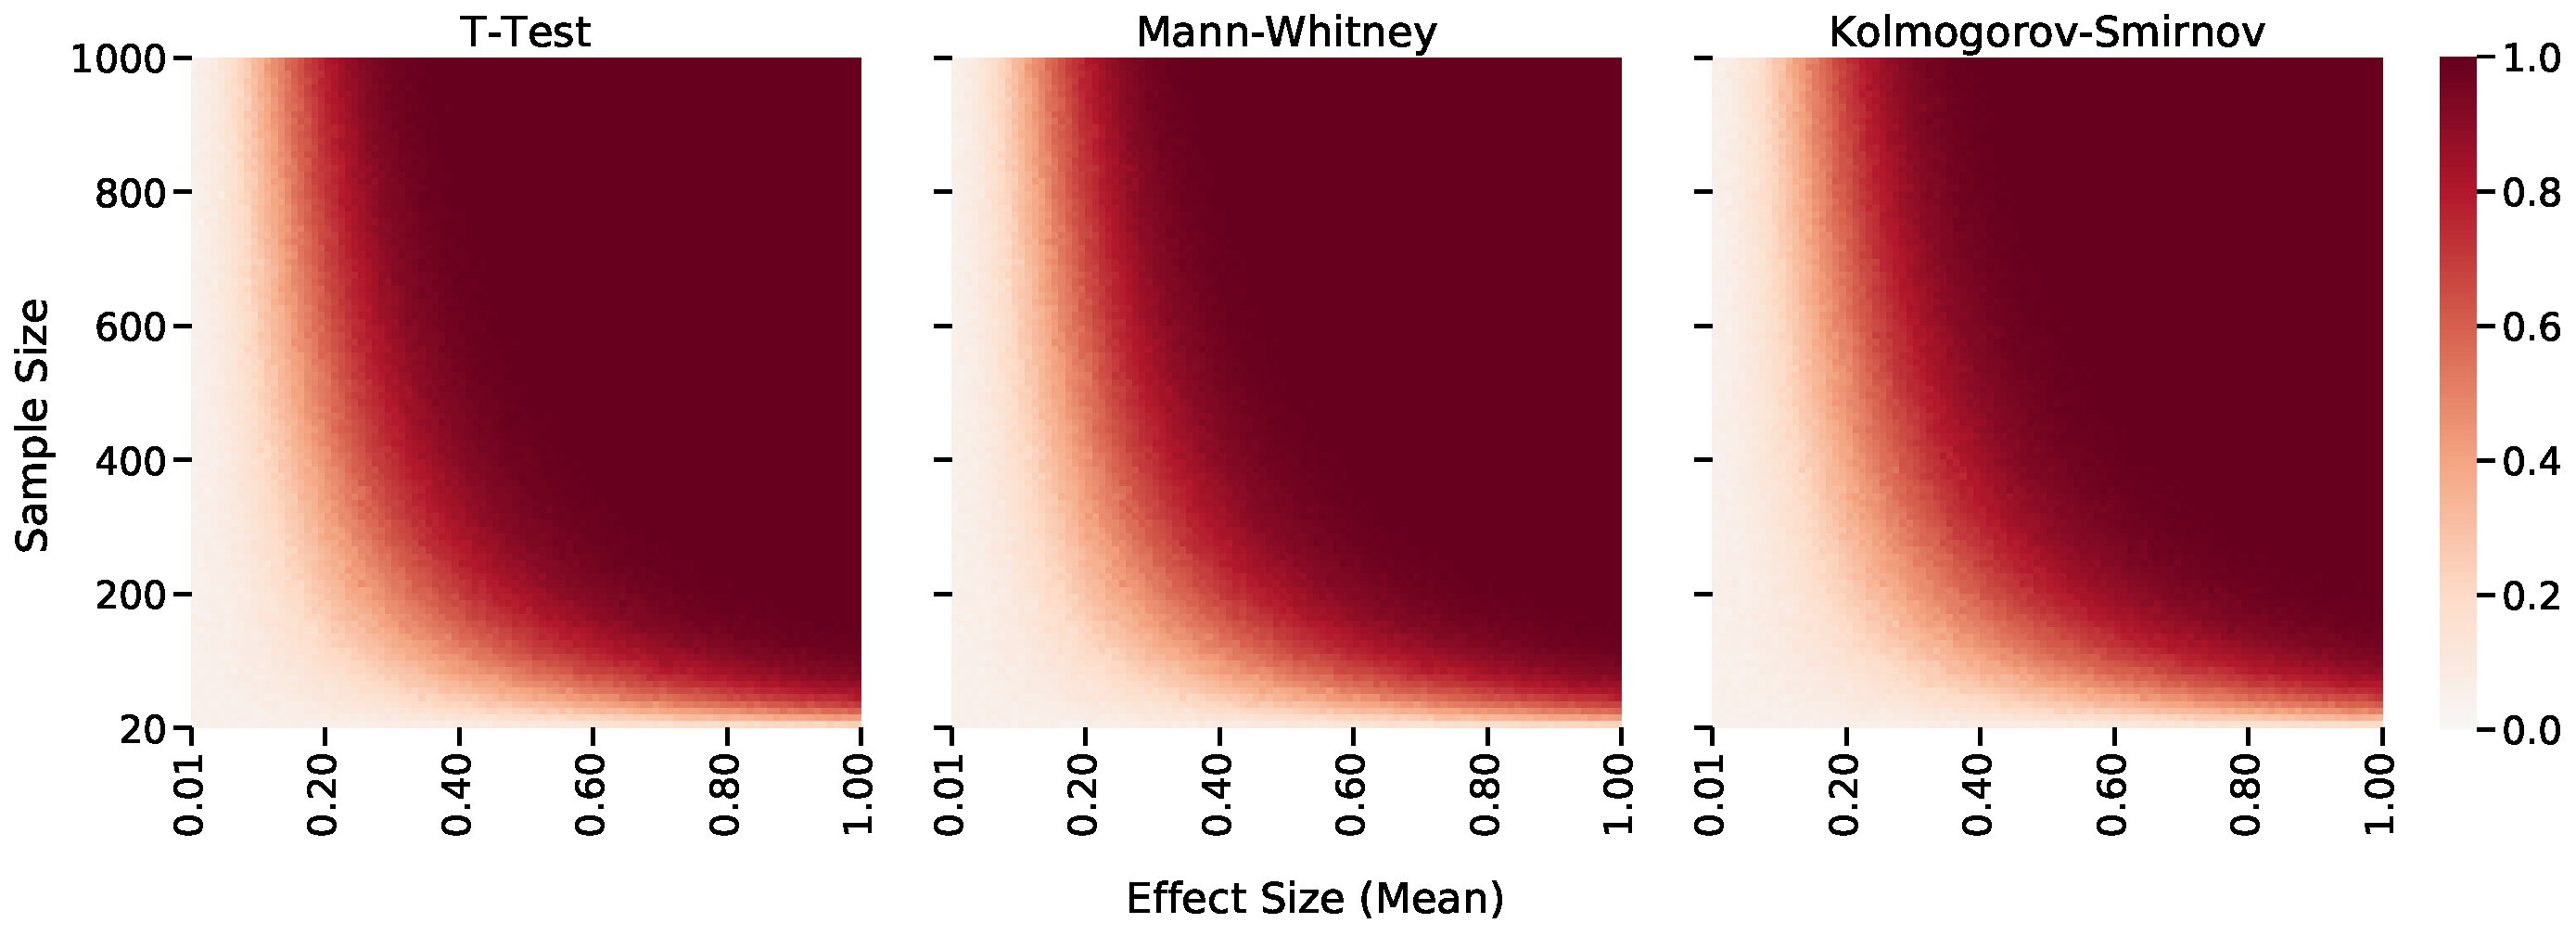
\includegraphics[width=.9\textwidth]{figures/exp2_change_mean}
    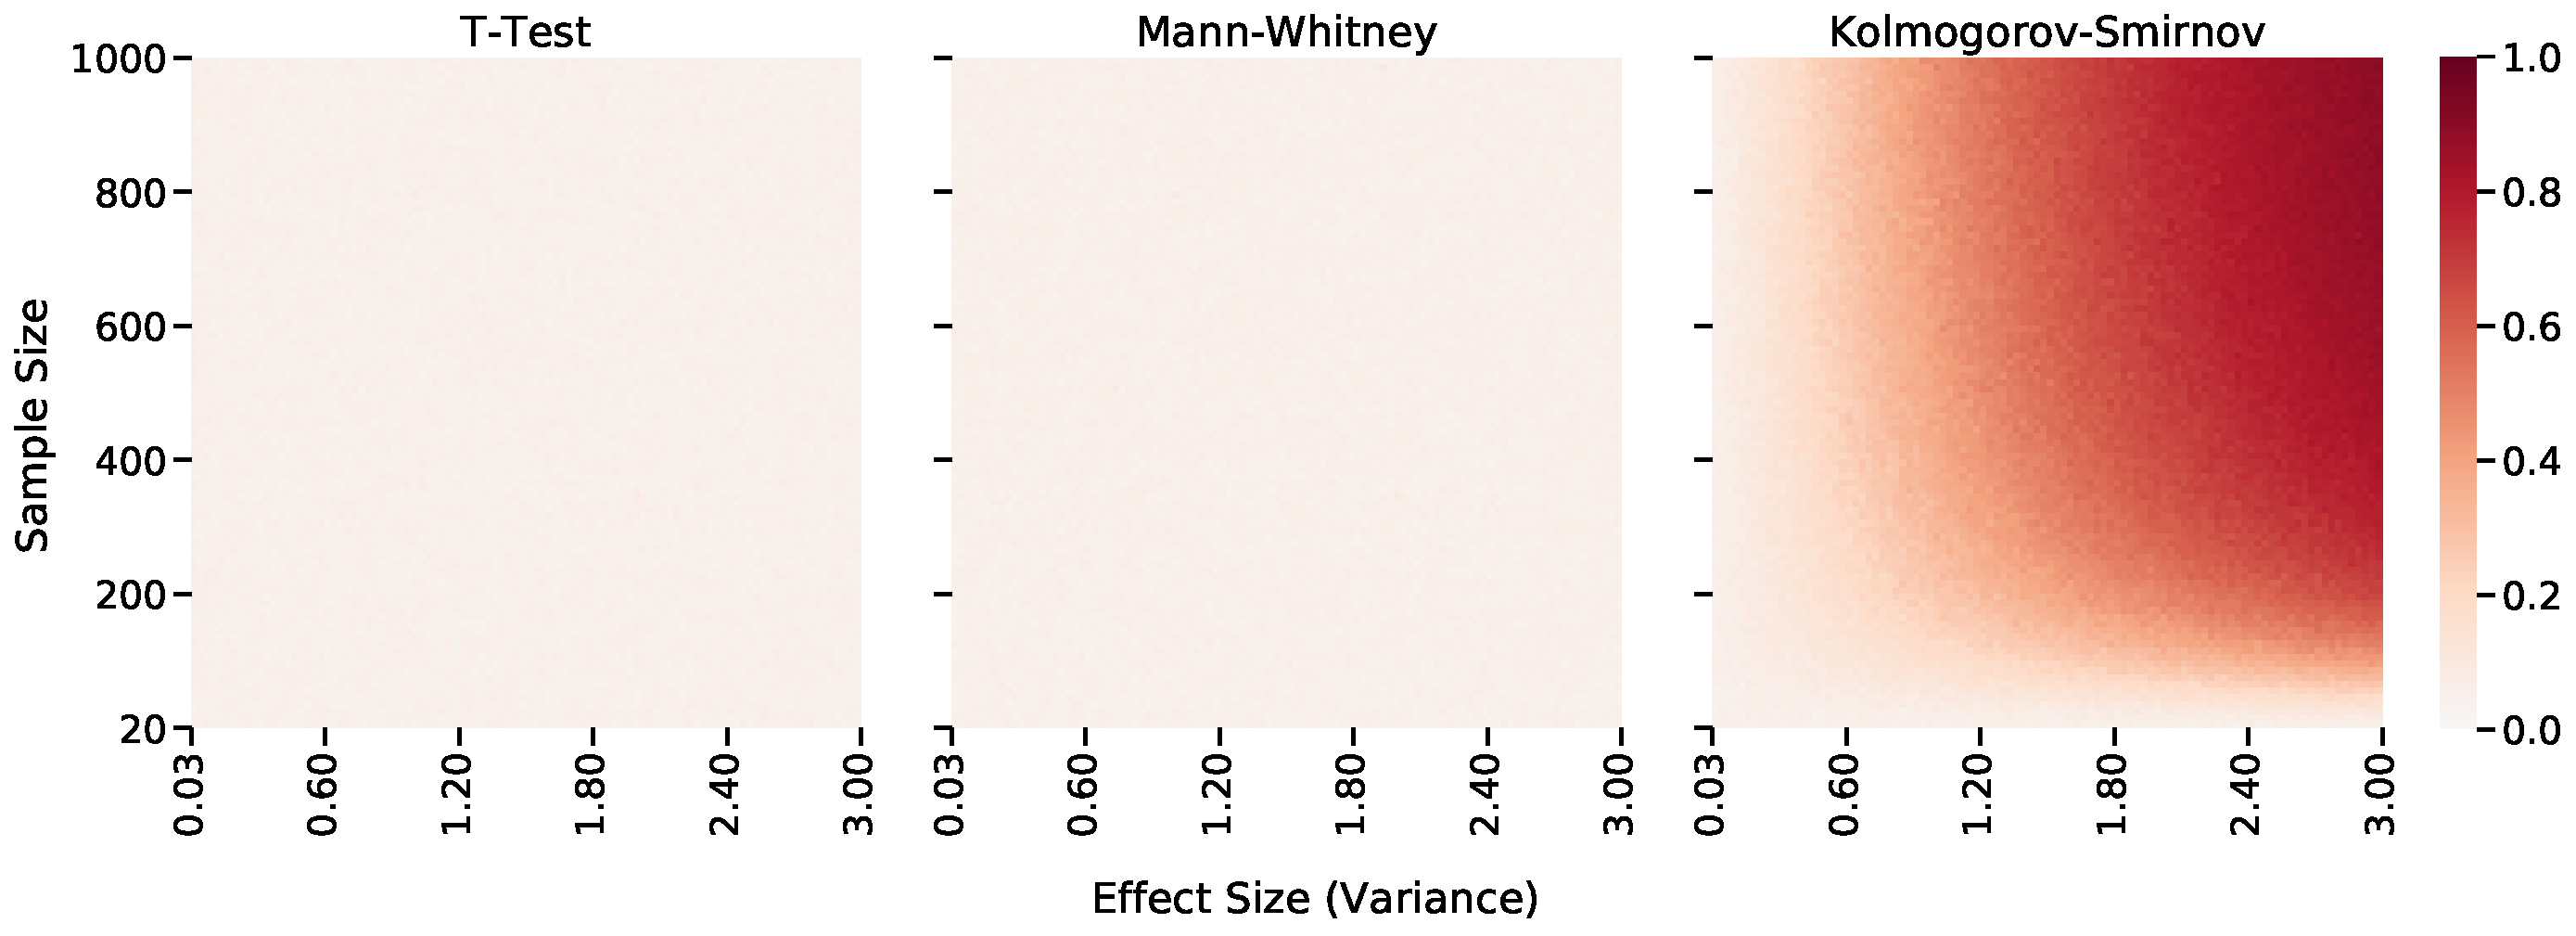
\includegraphics[width=.9\textwidth]{figures/exp2_change_vars}
    \caption{
    \textbf{Performance of finding significant edges that have different weight distributions.}
    Recall@10 for each edge when comparing two populations of weighted networks using t-test, Mann-Whitney, and Kolmogorov-Smirnov tests. The color bar represents recall averaged over 100 trials. 
    \textit{(Top row)} Results for varying the mean $\delta$ and sample size wile keeping the variance is same ($\phi = 0$). All three tests perform equally, and can detect significant edges when edge distributions differ in means.
    \textit{(Bottom row)} Results for varying the variance $\phi$ and sample size wile keeping the mean same ($\delta = 0$). T-test and Mann-Whitney test cannot detect changes in variance regardless of the sample and effect size. KS test is the only test that can detect changes in variance.}
    \label{fig:exp2}
\end{figure}

Functional connectivity in human brains was analyzed using functional connectomes estimated using fMRI data from the HCP dataset. In functional connectomes, the edges represent correlations of changes in blood flow between a pair of ROIs, which is a proxy for correlations of brain activity. For each edge, the class-conditional mean and the variance of truncated normal distribution are computed for males ($m=330$) and females ($m=407$). Networks are then simulated as above using the 2-block weighted $\sbm$, but the parameters for first block, $\B_{11}$, is substituted with class-conditional means and variances. The performance is measured with recall@10, denoted empirical trustworthiness in Figure \ref{fig:exp2_hcp}, is measured using KS test. Again, the empirical trustworthiness shows how one can trust that the edge is truly different. There are 70 vertices with 2380 total edges, but only 256 edges have trustworthiness $\geq 0.9$.

\begin{figure}
    \centering
    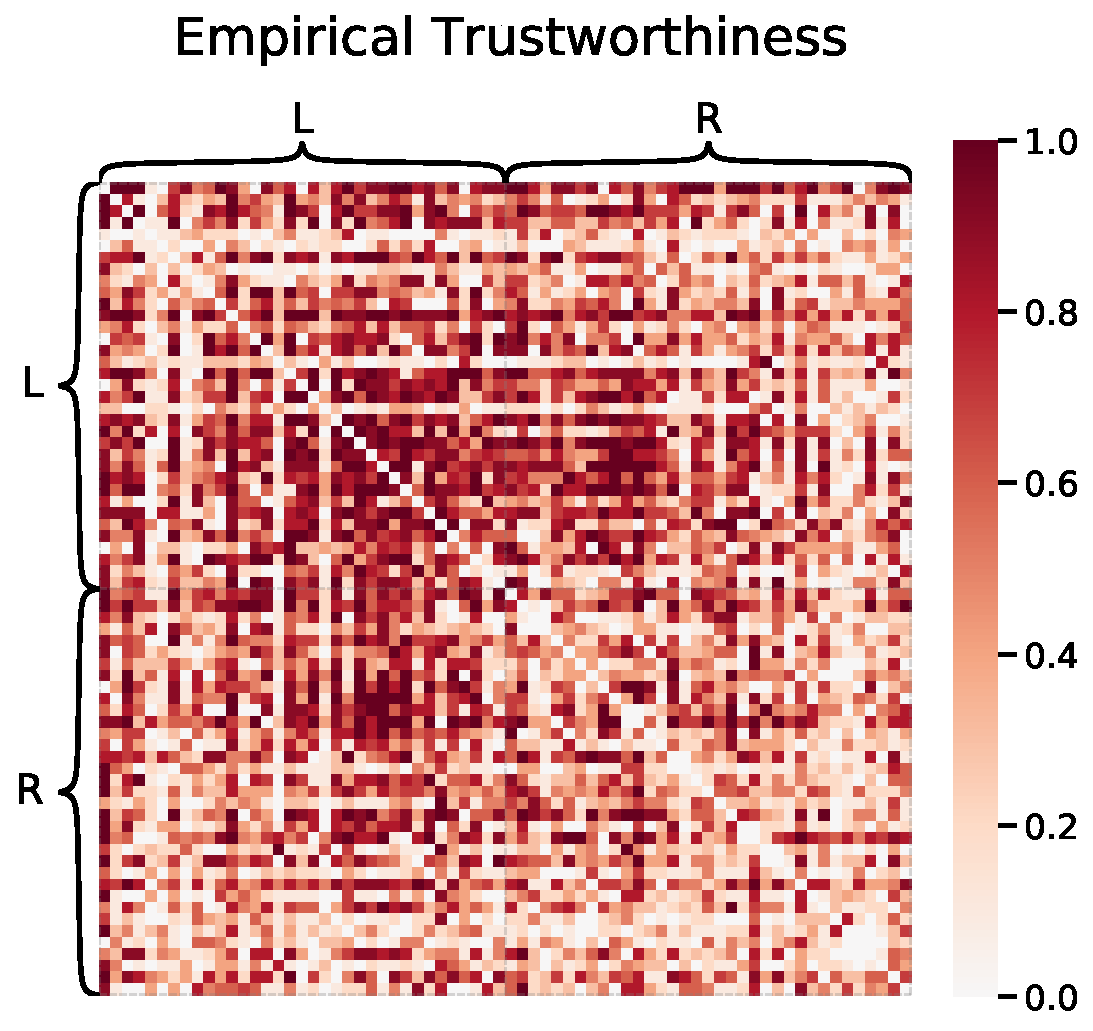
\includegraphics[width=0.45\textwidth]{figures/exp2_empirical_trustworthiness}
    \caption{
    Functional connectomes are derived from the HCP data. Vertices are defined by Desikan parcellation into 70 ROIs, and are organized by hemisphere, denoted left hemisphere (L) and right hemisphere (R). Edge weights are correlations represent correlation of brain activity between a pair of ROIs. 
    For each edge, the class-conditional means and the variances for females ($m=407$) and males ($m=330$) are computed, which are used to simulate weighted 2-block $\sbm$. Recall@10, denoted empirical trustworthiness, is measured from test statistics using KS test. Out of the 2380 total edges, only 256 edges have trustworthiness $\geq 0.9$. 
    }
    \label{fig:exp2_hcp}
\end{figure}


% \begin{summary}[SUMMARY POINTS]
% When comparing two populations of weighted networks for significantly different edges, t-test can detect changes in means, but cannot detect changes in variances. Distribution free tests, such as Kologrov-Smirnov test can detect changes in both means and variances.
% \end{summary}

\subsection{Testing for Significant Edges Using Communities in Binary Networks} \label{sec:exp3}
In previous section \ref{sec:exp1}, the community structure was ignored even though the generative process produced two communities. In the following experiment, the community assignments are used to test whether all edges within a community or across communities are significantly different. Formally, the following hypothesis test is considered: 
\begin{align*}
    H_0:~ \PP[\B_{ij}|Y=0] = \PP[\B_{ij}|Y=1]\\
    H_A:~  \PP[\B_{ij}|Y=0]\neq \PP[\B_{ij}|Y=1]
\end{align*}
where $\PP[\B_{ij}|Y=y]$ denotes class-conditional distribution of edges that belong to community $i$ and $j$, and $i, j\in [K]$ where $K$ denotes the number of communities. When $i =j$, the edges are incident to vertices that belong to the same community. When $i\neq j$, the edges are incident to vertices that do not belong in the same community. In this setting, a total of $\frac{(K)(K+1)}{2}$ null hypothesis are tested.  

We consider two populations of networks with the connectivity probability matrices as below, 
\begin{align*}
\B^{(1)} = 
    \begin{bmatrix}
    p & p \\ p & p
    \end{bmatrix},~
\B^{(2)} = 
    \begin{bmatrix}
    p+\delta & p \\ p & p
    \end{bmatrix}
\end{align*}
with $n=50$ vertices, and membership vector, $\vec{\pi} = \bracks*{0.5, 0.5}$. Total of $m$ networks are sampled ($m/2$ networks per population). Since $K=2$, community assignment results in three sets of edges, two within communities and one across communities. The t-test statistic was computed for each set of edges, and significant edges are identified by the hypothesis test that resulted in largest test-statistic. The performance is measured by precision, which measures false positive rate, and recall, which measures true positive rate.

Figure \ref{fig:exp3} shows the results of using t-test as the effect size is changed using known and estimated community assignments. When the community assignment is known \textit{a priori}, significant edges can be perfectly detected with no false positives at low sample sizes ($m=10$) and effect size ($\delta \geq 0.05$). However, estimating community assignments results in large number of false positives edges as shown in precision plots for both $\jrdpg$ and $\cosie$ models since recovery of community assignments is correlated with magnitude of the effect size. When effect size is small, communities cannot be reliably recovered for both $\jrdpg$ and $\cosie$ models, which results in false positive tests. As effect size increases, community recovery improves and the number of false positive edges decrease at effect size ($\delta \geq 0.2$). 

\begin{figure}
    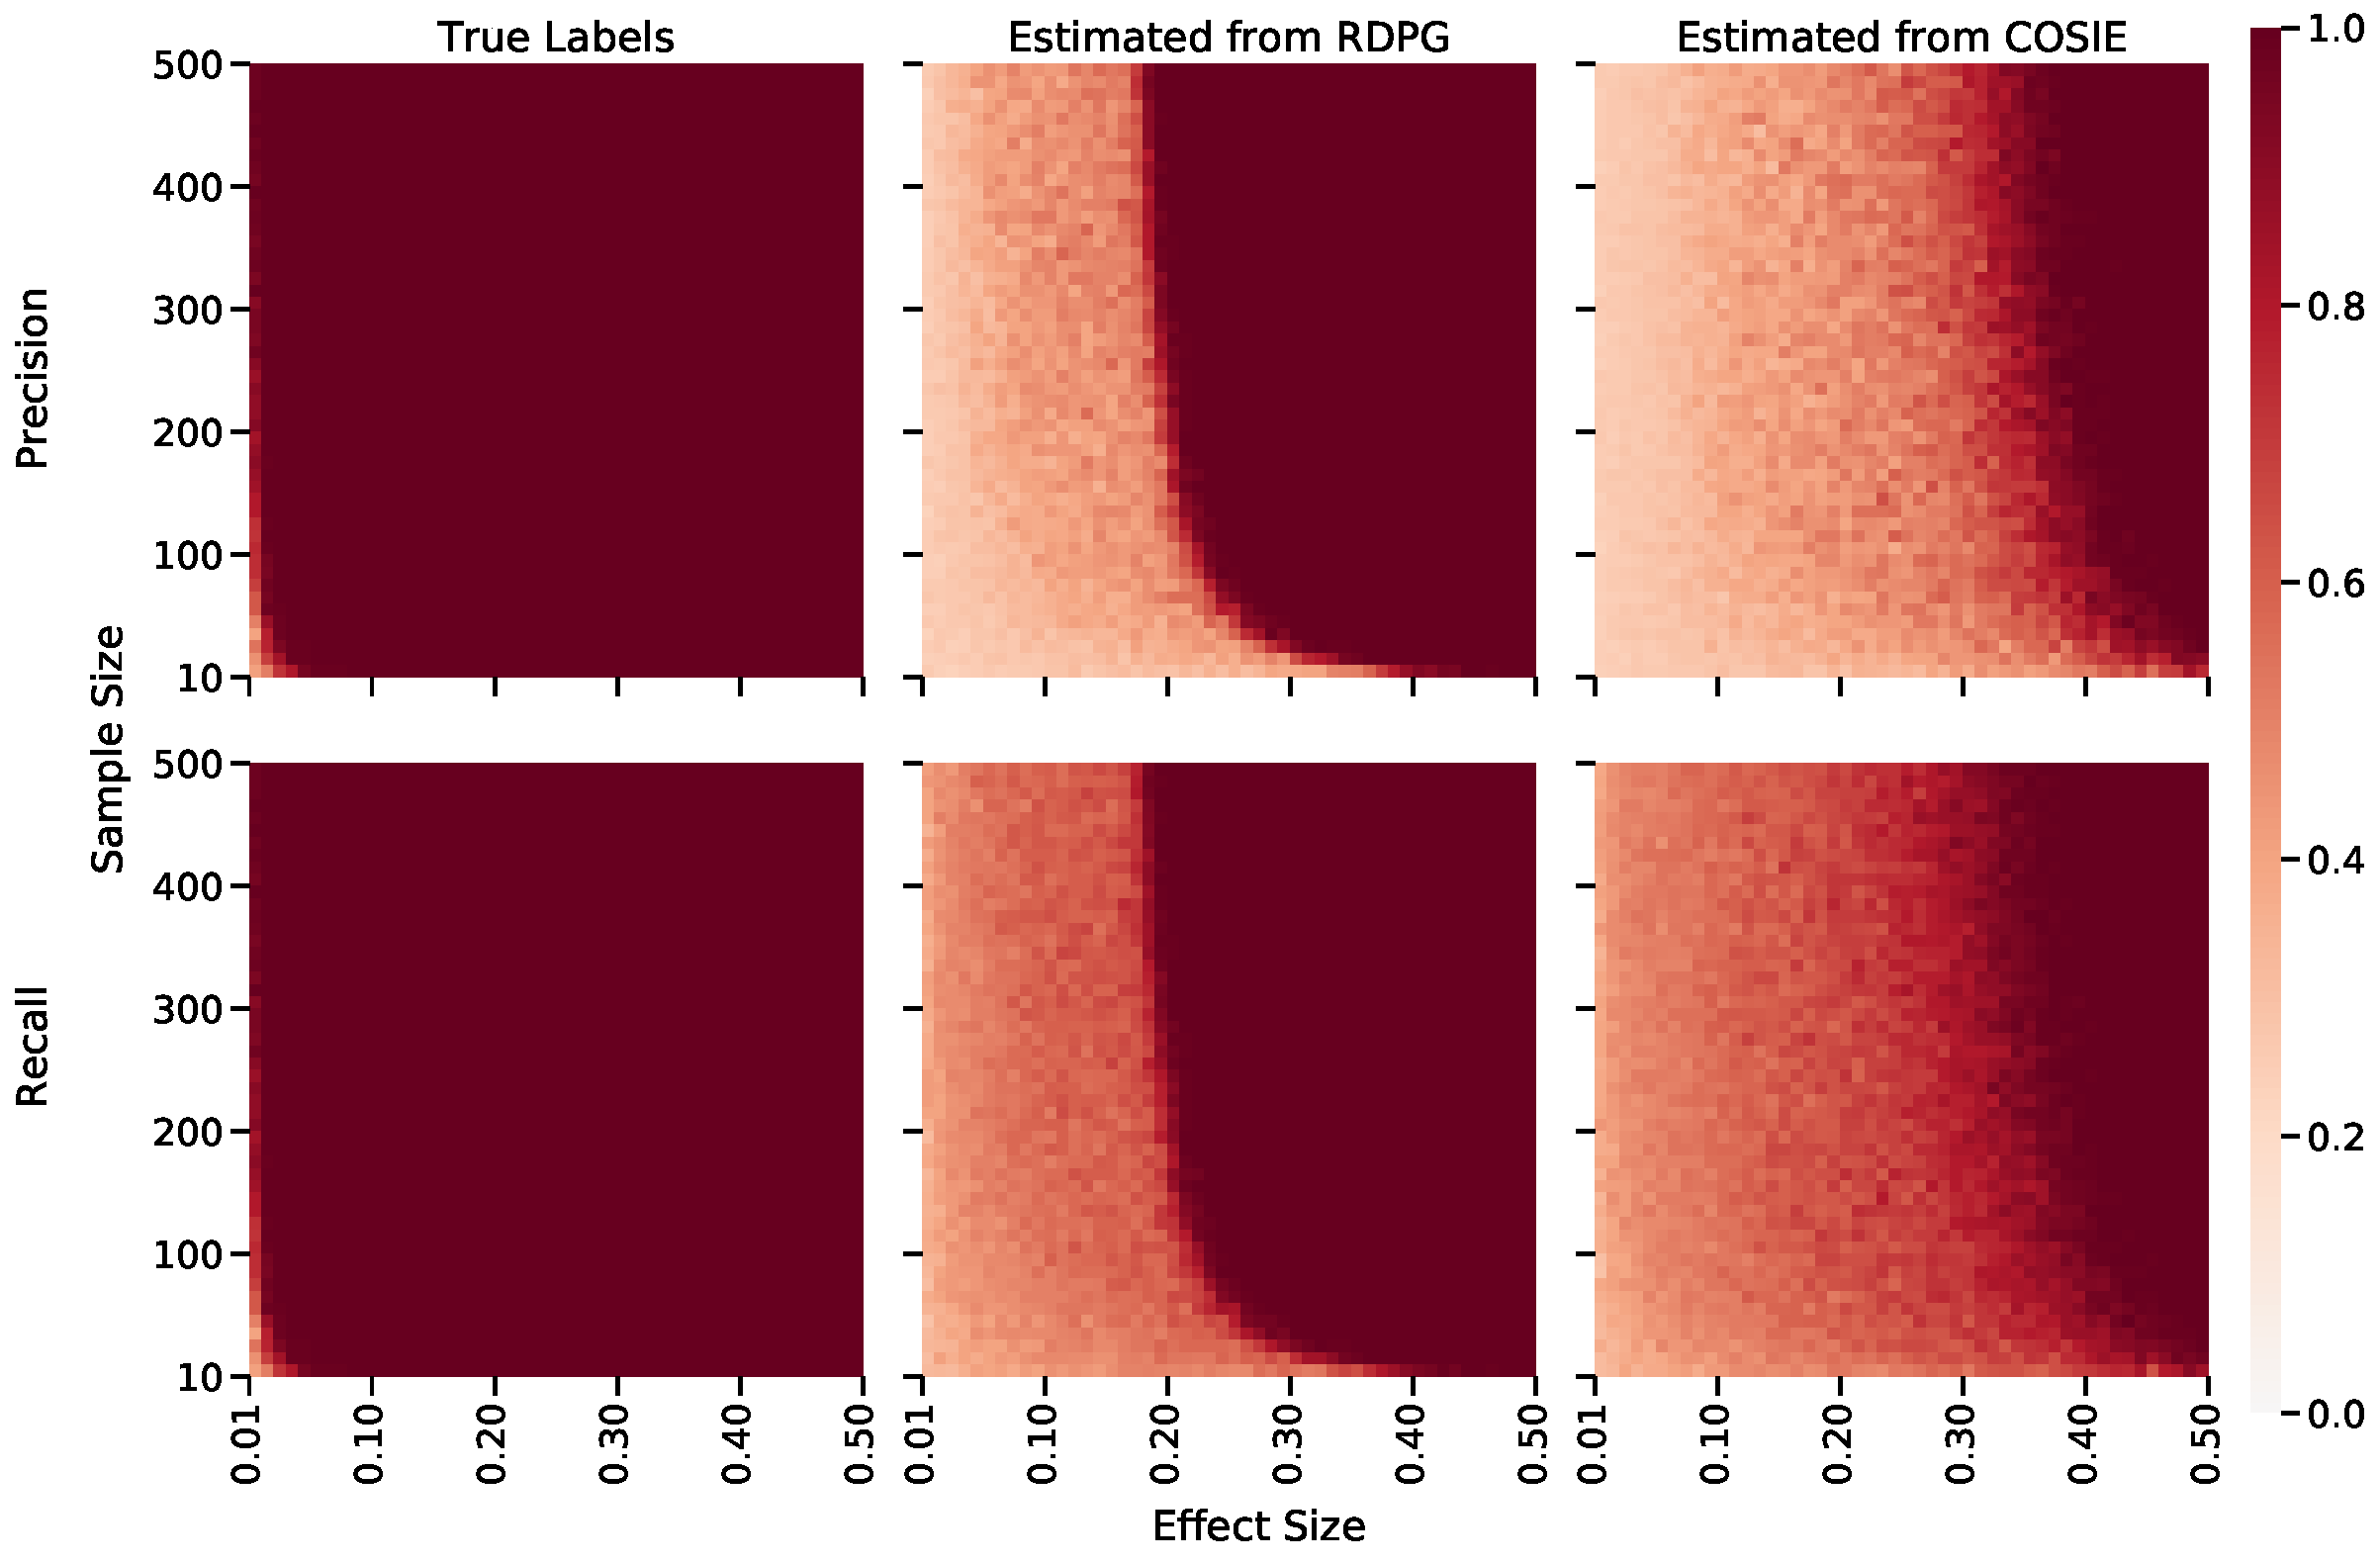
\includegraphics[width=.9\textwidth]{figures/exp3_final}
    \caption{
    \textbf{Performance of finding significant edges using either known or estimated community structure.}
    Precision \textit{(top row)} and recall \textit{(bottom row)} for
    significant edges using t-test on sets of edges from within community or across communities averaged over 50 trials.
    \textit{(Left column)} shows the precision and recall when using true community assignments. At low sample sizes ($m =10$) and low effect size ($\delta \geq 0.05$), community wise testing results in perfect precision and recall.
    \textit{(Middle column)} shows the results for using community assignments estimated under the $\jrdpg$ model. 
    \textit{(Right column)} shows the results for using community assignments estimated under the  $\cosie$ model. 
    Since recovery of community assignment is related to the effect size, spectral clustering results in misclassified vertices. As a result, precision is low at effect sizes $\leq 0.2$. As effect size increases, the communities become more identifiable, and results in increased precision for $\jrdpg$ and $\cosie$ models. However, COSIE model requires larger effect size to reach precision $\geq 0.95$.
    }
    \label{fig:exp3}
\end{figure}


% The same analysis was performed using binarized structural connectomes from HCP dataset where the connectivity within and across communities are tested between females ($m=407$) and males ($m=407$). Using known hemispheric labels of the vertices, the class-conditional block probabilities are computed and used to simulate 2-block SBMs, and the precision and recall was measured for each hypothesis test. Table \ref{tab:exp3_hcp} shows that in the suggesting that there are differences in the connectivity with and across hemispheres are significantly different in males and females. 

% \begin{table}
%     \caption{Empirical trustworthiness computed using structural connectome from HCP dataset.}
%     \centering
%     \begin{tabular}{c|c|c}
%         \toprule
%         Hypothesis Test &  Empirical Precision & Empirical Recall\\
%         \midrule
%         Right vs Right  &   1   &   1\\
%         Left vs Left    &   1   &   1\\
%         Left vs Right   &   1   &   1\\
%         \bottomrule
%     \end{tabular}
%     \label{tab:exp3_hcp}
% \end{table}

% Show the magnitudes of the test statistics 

% \begin{summary}[SUMMARY POINTS]
% Using community assignments can improve detection of significant edges. When community assignment is know beforehand, community-wise testing can detect significant edges at low sample and effect sizes. 
% When community assignment is not know beforehand, it can be estimated using statistical models. However, community assignment cannot always be trusted, and consequently any subsequent inference, since its performance depends on effect size.
% \end{summary}



\subsection{Testing for Significant Edges Using Communities in Weighted Networks} \label{sec:exp4}

We consider weighted 2-block $\sbm$ similar to that of Section \ref{sec:exp2}, but with $n=50$ vertices, membership vector, $\vec{\pi} = \bracks*{0.5, 0.5}$, and block edge distribution is as below: 
\begin{align*}
    \B^{(1)} &= 
    \begin{bmatrix}
        \tnorm(0, 0.25, -1, 1)   & \tnorm(0, 0.25, -1, 1) \\
        \tnorm(0, 0.25, -1, 1)   & \tnorm(0, 0.25, -1, 1) 
    \end{bmatrix} \\
    \B^{(2)} &= 
    \begin{bmatrix}
        \tnorm(0 + \delta, 0.25 + \phi, -1, 1)   & \tnorm(0, 0.25, -1, 1) \\
        \tnorm(0, 0.25, -1, 1)   & \tnorm(0, 0.25, -1, 1) 
    \end{bmatrix}
\end{align*}
We proceed with the same experiment as that of Section \ref{sec:exp3}, while changing the means ($\delta$) or the variances ($\phi$). The community assignment is estimated using $\omni$ under $\jrdpg$ model and $\mase$ under $\cosie$ model.
The KS test statistic was computed for each set of edges, and significant edges are identified by the hypothesis test that resulted in largest test-statistic.
The performance is measured with precision and recall. 

Figure \ref{fig:exp4_means} shows the results when varying the mean ($\delta$) and Figure \ref{fig:exp4_vars} shows the results when varying the variance ($\phi$). When the community assignment is known \textit{a priori}, significant edges can be perfectly detected with no false positives at low sample sizes ($m=10$) and effect size ($\delta \geq 0.1$, $\phi \geq 0.12$). When means are changed, communities can be perfectly recovered under $\jrdpg$ model, but communities cannot be reliably recovered under $\cosie$ model. When the edge distributions are different by variance, recovering communities is impossible regardless of the statistical model. This suggest that both $\jrdpg$ and $\cosie$ models are not appropriate when studying differences in variances. 

\begin{figure}
    \centering
    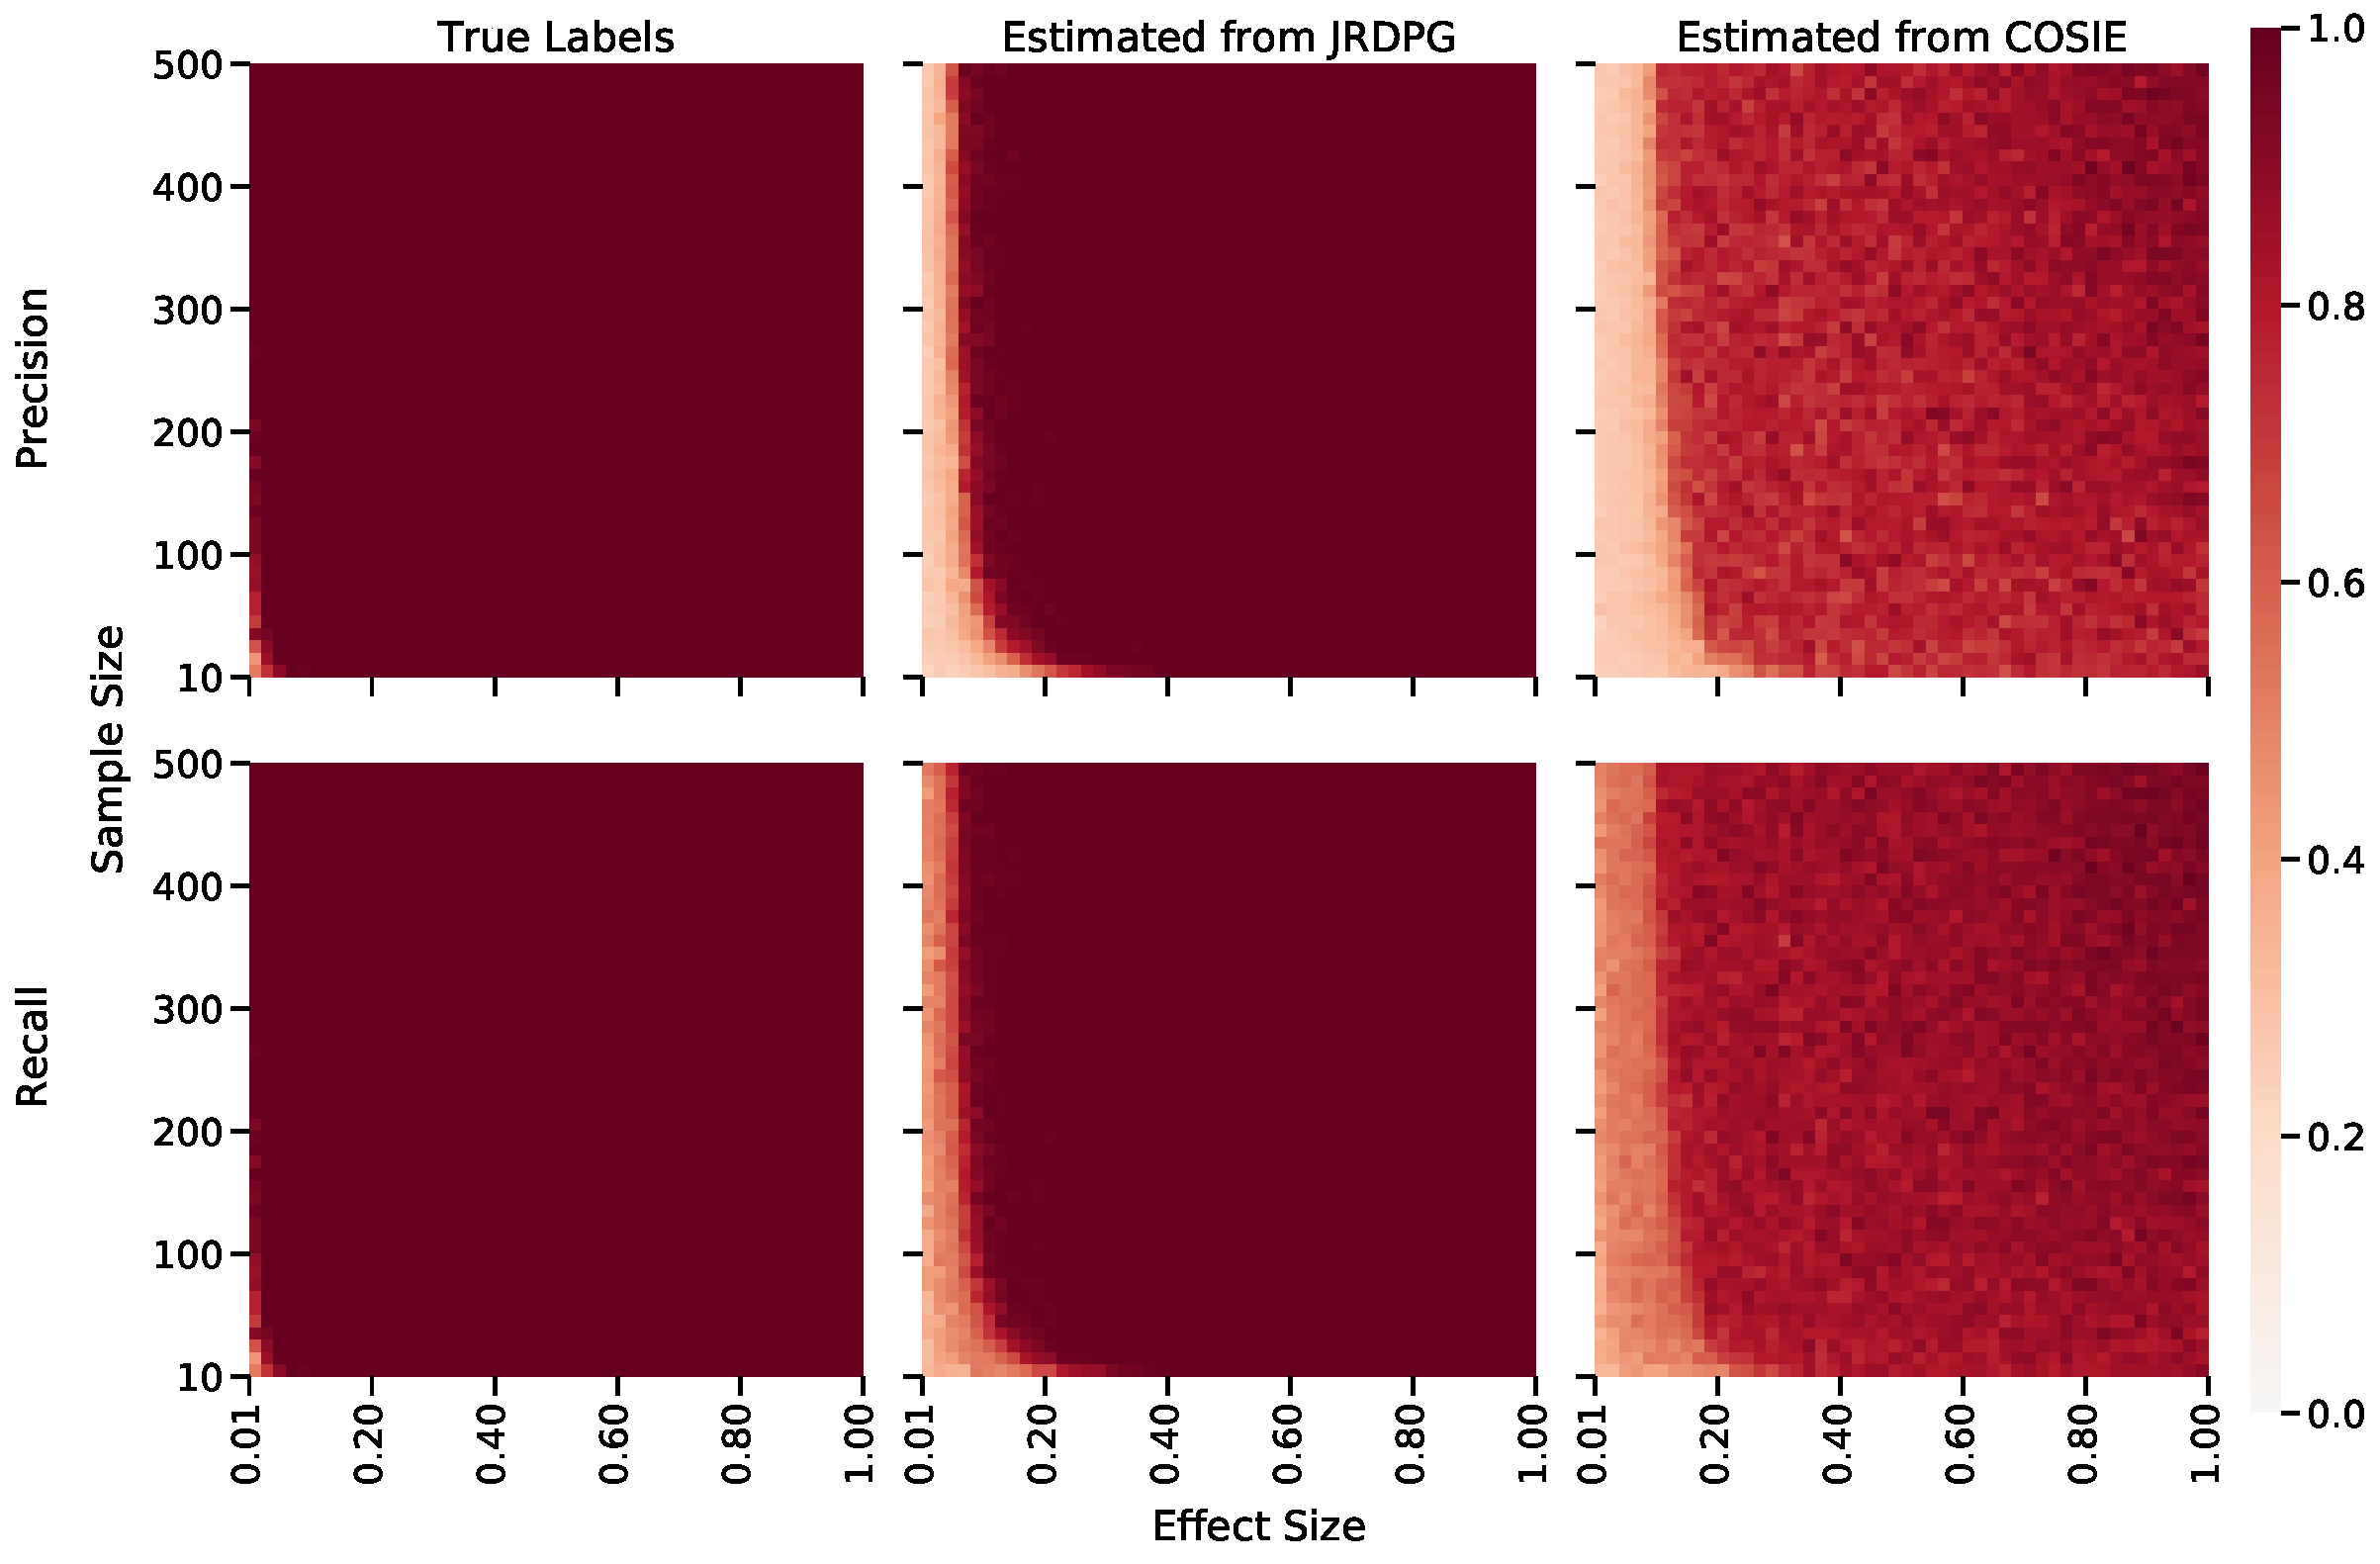
\includegraphics[width=.9\textwidth]{figures/exp4_means_final.pdf}
    \caption{Precision \textit{(top row)} and recall \textit{(bottom row)} for significant edges using $\ks$ test averaged over 50 trials. Effect size (x-axis) is the difference in means of the truncated normal distribution for $\B_{1, 1}$.
    \textit{(Left column)} shows the precision and recall when using known community assignments. At low sample sizes ($m =10$) and low effect size ($\delta \geq 0.1$), community wise testing results in perfect precision and recall.
    \textit{(Middle column)} shows the results for using community assignments estimated under the $\jrdpg$ model. Even at low effect size ($\delta \geq 0.15$), communities can be perfectly recovered. All significant edges can be detected without false positives. 
    \textit{(Right column)} shows the results for using community assignments estimated under the $\cosie$ model. Under this model, communities cannot be perfectly recovered, resulting in false positive edges and false negative edges.}
    \label{fig:exp4_means}
\end{figure}

\begin{figure}
    \centering
    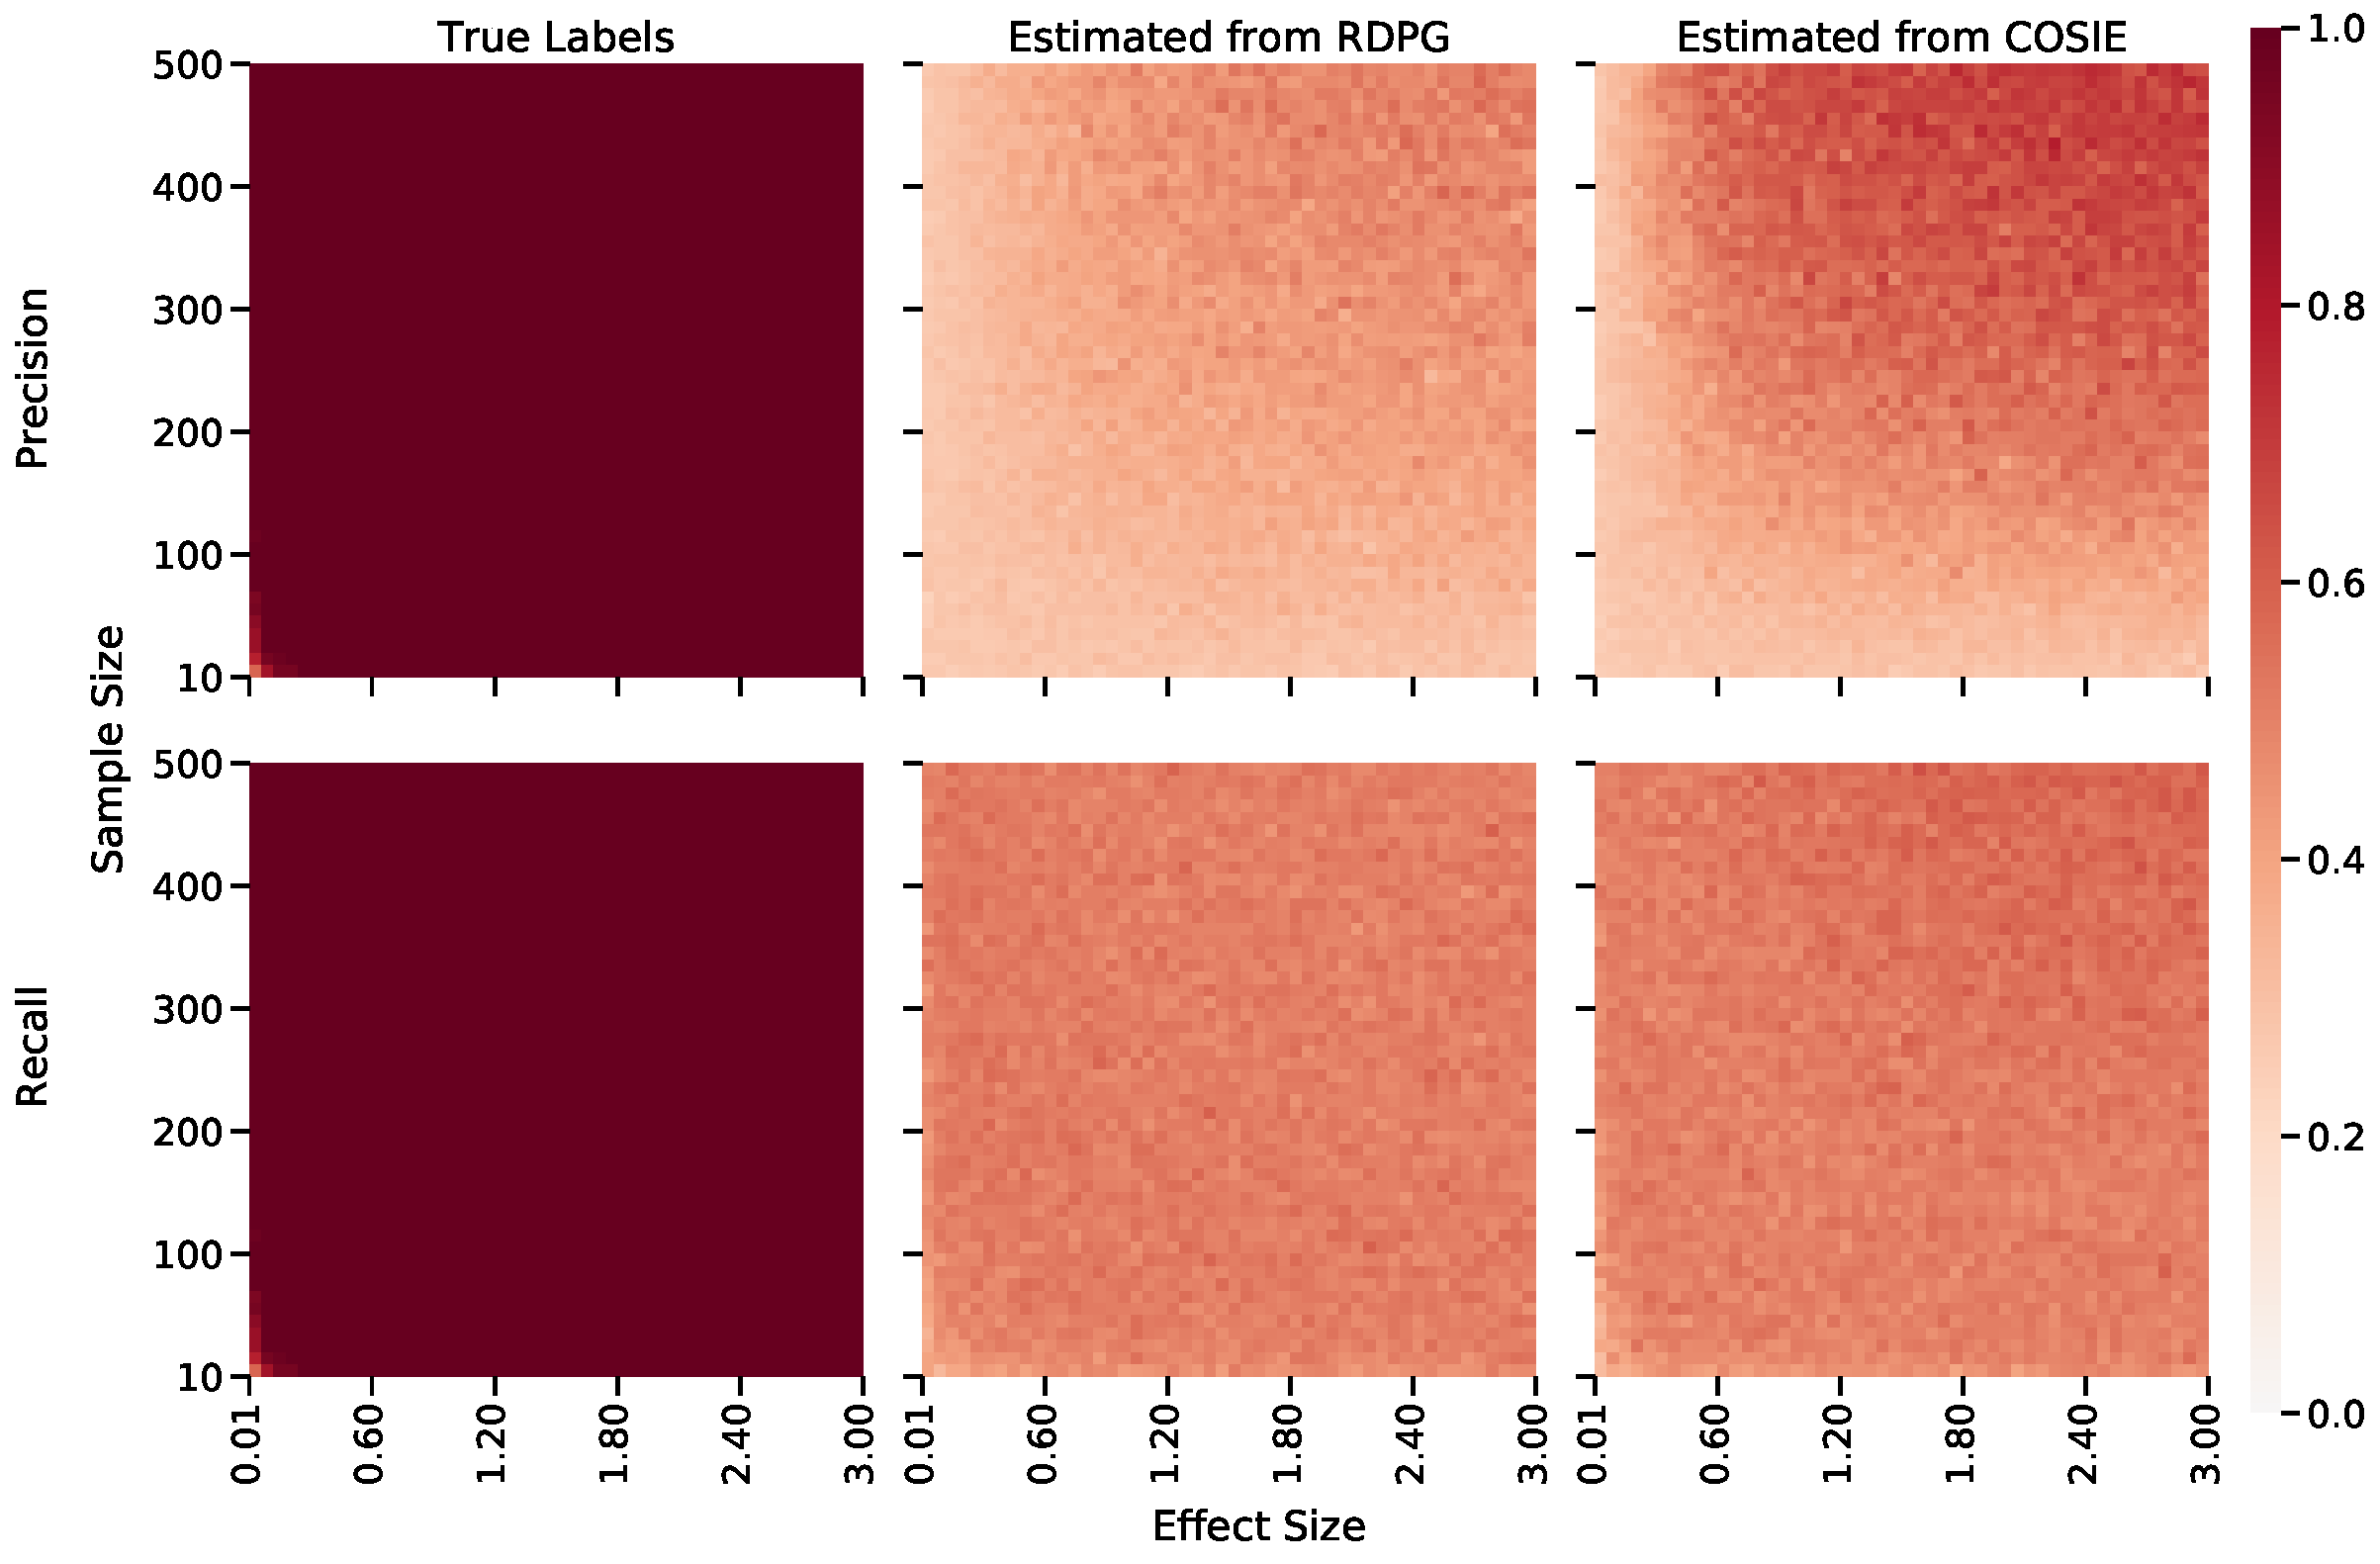
\includegraphics[width=.9\textwidth]{figures/exp4_vars_final.pdf}
    \caption{Precision \textit{(top row)} and recall \textit{(bottom row)} for significant edges using $\ks$ test sets on of edges from within community or across communities averaged over 50 trials. Effect size (x-axis) is the difference in variances of the truncated normal distribution for $B_{1,1}$.
    \textit{(Left column)} shows the precision and recall when using known community assignments. At low sample sizes ($m =10$) and low effect size ($\phi \geq 0.12$), community wise testing results in perfect precision and recall.
    \textit{(Middle column)} shows the results for using community assignments estimated under the $\jrdpg$ model.
    \textit{(Right column)} shows the results for using community assignments estimated under the $\cosie$ model.
    Communities cannot be recovered under both $\jrdpg$ and $\cosie$ model regardless of effect size and sample size. As a result, community-wise testing result in large number of false positive edges.
    }
    \label{fig:exp4_vars}
\end{figure}

% \begin{table}
%     \caption{Empirical trustworthiness computed using functional connectomes from HCP dataset.}
%     \centering
%     \begin{tabular}{c|c|c|c|c|c|c}
%         \toprule
%         \multirow{2}{*}{Hypothesis Test} &
%           \multicolumn{2}{c}{T-test} &
%           \multicolumn{2}{c}{Mann-Whitney} &
%           \multicolumn{2}{c}{Kologrov-Smirnov} \\
%          &  Precision & Recall & Precision & Recall & Precision &  Recall\\
%         \midrule
%         Right vs Right  &   x   &   x  \\
%         Left vs Left    &   x   &   x  \\
%         Left vs Right   &   x   &   x  \\
%         \bottomrule
%     \end{tabular}
%     \label{tab:exp4_hcp}
% \end{table}


% \begin{summary}[SUMMARY POINTS]
% Higher power in testing for significant edges can be achieved by comparing sets of edges rather than individual edges using community assignments.
% When community assignment must be estimated, both $\jrdpg$ and $\cosie$ models are appropriate when the edge distribution is different in means. However, both models are not useful when the edge distribution is different in variances.
% \end{summary}


